\documentclass[a4paper, 12pt, twoside]{report}
\usepackage[english]{babel} % en
\usepackage{graphicx}
\usepackage{hyperref}
\usepackage[T1]{fontenc}
\usepackage[utf8]{inputenc}
\usepackage{setspace}
\usepackage[paper=a4paper,margin=1in]{geometry}
\usepackage{parskip}
\usepackage{fancyhdr}
\usepackage[superscript]{cite}
\usepackage{units}
\usepackage[htt]{hyphenat}
\usepackage{enumitem}
\usepackage{wrapfig}
\usepackage{mathtools}
\pagestyle{fancy}
\PassOptionsToPackage{hyphens}{url}\usepackage{hyperref}

\begin{document}
	
	\begin{titlepage}
		
		\begin{minipage}[t]{0.19\textwidth}
			\vspace{-4mm}{
\includegraphics[scale=1.15]{images/logo_unimib.pdf}}
		\end{minipage}
		\begin{minipage}[t]{0.81\textwidth}
			{
				\setstretch{1.42}
				{\textsc{Università degli Studi di Milano - Bicocca}} \\
				\textbf{Scuola di Scienze} \\
				\textbf{Dipartimento di Informatica, Sistemistica e Comunicazione} \\
				\textbf{Corso di laurea in Informatica} \\
				\par
			}
		\end{minipage}
		
		\vspace{40mm}
		
		\begin{center}
			{\LARGE{
					\setstretch{1.2}
					\textbf{A Data Analytics Framework for \\Medical Prescription Pattern Dynamics}
					\par
			}}
		\end{center}
		
		\vspace{40mm}
		
		{\large \textbf{Relatore:} Prof. Francesco Archetti \medskip} \\
		{\large \textbf{Correlatore:} Prof. Paolo Mariani \medskip} \\
		{\large \textbf{Tutor aziendale:} Dott. Gaia Arosio \medskip} \\
		
		\vspace{15mm}
		
		\begin{flushright}
			{\large \textbf{Relazione della prova finale di:}} \\
			\large{Ilaria Battiston} \\
			\large{Matricola 816339} 
		\end{flushright}
		
		\vspace{30mm}
		\begin{center}
			{\large{\bf Anno Accademico 2018-2019}}
		\end{center}
		
		\restoregeometry
		
	\end{titlepage}
    
\cleardoublepage
grazie CNR <3

ricordiamoci di mettere laura nei ringraziamenti
\cleardoublepage
\begin{abstract}
	Research on prescription pattern dynamics exploits medical information to highlight the issues concerning the growing antibiotic resistance among the Italian country, using a subset of data regarding the Campania region.
	
	After a clear understanding of the problem and the available information, along with its quality and feasible outcomes, a first analytical approach allows reconstruction of diagnosis and prescriptions global trending, from which is possible to extract patient journeys and underline changes.
	
	A deeper insight on antibiotics verifies national studies on overprescription, giving additional information on general practitioners' behaviour, brands popularity and seasonality of prescriptions, obtained with time series analysis and clustering.
\end{abstract} % rivedere
\cleardoublepage
\setcounter{tocdepth}{0}
\tableofcontents
\newpage
% mettere grassetto e corsivo ovunque
% titoli delle figure e tabelle con source (medical data etc)

\chapter{Introduction}
\section{Antibiotic resistance and misuse}
Antimicrobial resistance is a rising global problem which threatens the effective prevention and treatment of an ever-increasing range of infections caused by bacteria, parasites, viruses and fungi\cite{who}. 

Microorganisms exposed to antimicrobial drugs develop the ability to defeat substances designed to kill them, making infections persist in the body due to the unsuccessful action of agents.

This issue threatens public health causing higher healthcare costs to treat patients, and potentially compromising surgeries and chemotherapy results due to the ineffectiveness of antibiotics. No one can completely avoid the risk of resistant infections, but some people are at greater risk than others (for example, people with chronic illnesses)\cite{cdc}.

Antimicrobial resistance occurs naturally over time, usually through genetic changes. However, \textbf{the misuse and overuse of antimicrobials is accelerating this process}. In many places, antibiotics are overused and misused in people and animals, and often given without professional oversight\cite{who}.

Infections such as the common cold or sore throats are often countered with antibiotics, which have no effect against viruses and could as well put patients at the risk of suffering adverse reaction\cite{bmj}.

Therefore, to minimise the development of resistance, contributing factors must be reduced, optimising the use of drugs. This work requires effective surveillance and follow-up of consumption, at a local and national level. 

To be effective in the long run, work to optimise use of antibiotics must influence the prescribing practices of individual physicians. The goal is “rational use”, i.e. the correct patient receives the correct antibiotic at the correct dose and for the correct duration of treatment, in accordance with evidence-based guidelines. Over-prescribing should be avoided without resulting in under-prescribing\cite{sweden}.

Such work should be carried out close to the prescriber, something which also requires high resolution prescription data, down to the clinic and health centre level or better still at the level of \textbf{individual prescribers}.

\section{National Sanitary Service in Italy} % finire
The Italian National Sanitary Service (SSN) consists the complex of functions, activities and healthcare services offered by the State. It is based on subsidiarity, a general principle of the European Union law, stating that a central authority should have a subsidiary function, performing only those tasks which cannot be performed at a more local level\cite{oxford}.

SSN is articulated in different responsibility levels divided among the State, Regions, institutions and organisations, along with private structures and the Health Ministry, which coordinates the national sanitary plan.

Citizens benefit of healthcare services paying a related ticket\cite{ticket}, which represents the established way to contribute to expenses. It is used for:
\begin{itemize}
	\item Specialist examinations;
	\item First-aid help in non-emergency situations;
	\item Thermal care.
\end{itemize}

General practitioners' visits are exempted from payment of tickets. 
% tickets, ruolo del medico di base (prescrive le ricette) in modo generico, tanto c'è scritto dopo

\subsection{Drugs and prescriptions}
% AIFA
% prescrizioni di farmaci etici (scenario, evoluzione del settore) 30 pagine
%Rapporti di farmindustria, siti ministero Salute, agenas, federfarma

From the year 2000 every form of participation to sanitary expenses from citizens has been abolished\cite{ticket}, yet most Regions have introduced special drugs classes with a fixed quota for each medical prescription or package, to remedy the economic deficit. 

% le classi di farmaci sono: a, h, ???

% farmaci generci

\subsection{Antibiotic resistance in Italy}

\section{Healthcare data}
%dati, collezione, come sono raccolti, open data in italia, società (aicuvia oims health), promofarma (farmacisti, organizza informaticamente i dati e li vende → aziende farmaceutiche), agenzia delle entrate (codice fiscale), spiegare come sono organizzati ecc
%3) proprietari sistemi sw di medicina generale, millennium
%3 canali di produzione del dato (medici, farmacisti, ae) + canale derivato aicuvia

\section{Data classification}
% idc9, atc, etc

\section{Healthcare analytics}
\textbf{Healthcare analytics} is a field of growing importance which allows a deep understanding of results collected in the healthcare area. 

Extracting insights can be a complex challenge: health big data gives a huge \textit{volume} and \textit{variety} of information, therefore accessing the resources in a quick way is necessary. 

Other issues to deal with are \textit{veracity}, \textit{validity} and \textit{viability}, fundamental characteristics to ensure reliable and relevant analytics. Checking for integrity and quality can be difficult to verify without domain knowledge\cite{4vs}.

One of the various applications of this field is the change of patterns in the historical data: this research specifically focuses on \textbf{prescription pattern changes} on chronic patients, highlighting the development of some common medicines through time.

The considered healthcare data is a dump of a database created and handled by Millennium Srl\cite{millewin}, a leader company in IT services for medicine. This has been obtained through an extraction procedure on the original DB, assigning unique names to each table and column.

There are five main necessary fields for analysis\cite{DC}:
\begin{enumerate}
	\item \textbf{Spatial data}, in different granularity levels;
	\item \textbf{Personal data} of patients;
	\item \textbf{Temporal data}, in a range from 2000 to 2018, for time-series analysis;
	\item \textbf{Pharmacotherapeutic data}, classifiable according to different identification codes;
	\item \textbf{Diagnostic data}, for cross-validation of diagnoses.
\end{enumerate}

The two main risks encountered while doing analysis are information loss and inappropriate prescribing, that compromise the quality of statistics. Data may be incomplete, biased or filled with noise: another goal of analytics is to contrast incompleteness and incorrectness, obtaining coherent and clear results.
 
\chapter{Goals definition} % finire da qui
\section{Methodologies}
A general practitioner can do a wide range of daily activities, consisting in:
\begin{itemize}
	\item 
\end{itemize}
This specifical research is focussed on doctor-patient relationships, in particular information concerning diagnoses and prescriptions and their changes according to habits, time and geographical area. 

The dataset is modelled in a relational schema, which allows organization of records in structures (tables) to maintain integrity and compatibility between different kind of fields. For a better fruition of the workload, table names have been changed to standard English keywords.




%Relazione, modello ER, db stratificato, soglia temporale (dati disponibili & usati: avvento del generico, 10 anni)
%Funnel, perdita progressiva di informazioni, aree individuate, patologie (atc, prodotti), analisi globali 

\section{Considerations}
Since health big data can provide a high variety of information, it is required to have some clear \textit{objectives} in mind to keep on track and avoid losing focus. 

The research is centred on the \textbf{changes of prescription patterns of antibiotics}: this is a wide goal, and more information is needed to achieve results. It's necessary to narrow the field down, only concentrating on some classes of medicines, and define subgroups of GPs and patients in a restricted amount of time.

To obtain constraints the more objective as possible, some further analysis can be useful. For instance, focussing on chronic patients is a relatively fast way to reduce the huge amount of rows to elaborate, but causes the loss of most information.

The first step to take, having a deep understanding of the data, is recognising the extent and impact of the \textbf{progressive information loss}, to define the final amount of clear records. Trying to fix mistakes is a risk, since the outcome could be incorrect, so deleting is the most practical option.

Removing unclear and futile data may not be enough to have consistent results: 18 years of data is a wide range, and \textit{splitting the dataset} or deciding to only consider a smaller scope can be beneficial for the analysis quality. 

Some constraints can be imposed on general practitioners as well: since the results have to be coherent and accurate, it's best practice to only consider \textbf{active GPs} with a \textbf{constant number of patients} (to be defined). \\ This would partially remedy the fact that doctors may have different approaches to the same disease.

The creation of cohorts (chronic patients) among the statistical population is an example of \textbf{cluster sampling}.

After the initial parsing, there will be a rough draft of the final result which then will be subject of the following steps:
\begin{enumerate}
	\item Further analysis on data correctness (record linkage);
	\item Elaboration of the statistics and time series clustering.
\end{enumerate}

Another relevant instance for analysis is the \textbf{subset} of diseases to consider: choices have to be made according to \textit{external studies}, \textit{marketing researches} and further \textit{discoveries on the provided data}. Focussing on the \textbf{most common ones} is a guideline to start.

Having an idea of which illnesses and prescription have unstable patterns might give a better vision, and can be done through statistics on the whole database. 

Some examples of analytics are:
\begin{itemize}
	\item Most common diseases through the years;
	\item Most common \textit{chronic} diseases through the years;
	\item Changes of the number of prescriptions for diseases in the same area;
	\item Changes of prescriptions based on the patient phenotype or market trends.
\end{itemize}

An obstacle to perceiving the meaning of results is the restricted domain knowledge: to compensate, confronting some experts in the field is required. The team comprehends computer scientists, statisticians, biologists and healthcare workers.

% spostare
The tools to analyse and elaborate the health data are:
\begin{itemize}
	\item \textbf{PostgreSQL}, for data management and querying;
		\begin{itemize}
			\item The software project to interface with the web server is \textbf{PgAdmin 4};
			\item All queries need to be optimized to avoid huge computational times, using indexes and Common Table Expressions;
		\end{itemize}
	\item \textbf{R}, for machine learning and graphics computing;
	\begin{itemize}
		\item There are many ways to create plots;
		\item Possible uses are time series analysis and trajectory clustering.
	\end{itemize}
\end{itemize}

Reports and slide-shares have been created and accessed using the \textbf{Google Suite}.

Due to the amount of sensitive data, detailed results are going to be omitted: the final conclusions will be a product of aggregation and schematisation.

\section{Practical goals}

\chapter{Data description}

\section{Overview of the database}
The database used for analytics contains data on medical histories of patients between \textbf{January 2000} and \textbf{October 2018.} 

It's important to note that the research work has been done on only a part of the whole database, consisting in \textbf{5 tables}. There is information available on \textbf{general practitioners}, \textbf{patients}, \textbf{diagnoses} and \textbf{prescriptions}: each macro-category is included in a separated table, so it's necessary to recognise the relationship between fields.

The 5 tables and their relative sizes are:
\begin{itemize}
	\item \textit{pazienti}, 1.015.618 tuples; \\
	Basic information about patients, identified by an encrypted UID;
	\item \textit{nos\_002}, 1.015.618 tuples; \\
	Extension of \textit{pazienti} with the same key, containing more detailed information and linkage with GPs;
	\item \textit{cart\_pazpbl}, 15.460.199 tuples; \\
	Information about diagnoses and relative description;
	\item \textit{cart\_terap}, 118.716.403 tuples; \\
	Information about therapies and prescribed medicines;
	\item \textit{cart\_accert}, 151.478.456 tuples; \\
	Information about medical checks and examinations.
\end{itemize}

It's easy to see that the number of rows is varying a lot: there are a lot more prescriptions than diagnosis, and 150 millions of medical examinations. 

Each diagnosis, prescription and examination is uniquely distinguished by the triplet patient-GP-date, which maps to \textit{codice--userid--time\_last} in the database. 

There are many other date fields, but \textit{time\_last} (last update of the record) is the only one of type \textit{timestamp}, making each one different from the others (it's unlikely to have a diagnosis or prescription for the same patient, by the same doctor and at the same exact moment). 

Analysis is performed using dates in the \textit{YYYY-MM-DD} format, since there's no need of unique data: there are lots of different prescription for the same patient made on the same day.

\section{Description of the tables}
Below is reported a brief description of the 5 tables, along with the main fields used for analytics and their meaning.

\subsection{\textit{pazienti}}
The table \textit{pazienti} includes information about patients. To maintain privacy, there are no real names: everything is \textbf{encrypted} as a 22-character string containing letters, numbers and special symbols.

Other relevant fields are:
\begin{itemize}
	\item \textit{data\_open}, date of beginning of the doctor-patient relationship;
	\item \textit{nascita}, date of birth;
	\item \textit{decesso}, eventual date of death;
	\item \textit{comune\_di\_nascita}, name (and code) of the birth municipality;
	\item \textit{sesso}, birth sex;
	\item \textit{pa\_convenzione}, type of convention with the Italian insurance system.
\end{itemize}

\subsection{\textit{nos\_002}}
The table \textit{nos\_002} contains the same information as \textit{pazienti}, with additional fields which are essential to analyse data:
\begin{itemize}
	\item \textit{pa\_medi}, \textbf{encrypted} UID of the general practitioner of the patient;
	\item \textit{pa\_cap}, zip-code of the patient (for geographical analysis);
	\item \textit{pa\_pro}, province of the patient;
	\item \textit{pa\_drevoca}, eventual date of termination of the doctor-patient relationship (a patient changing GP).
\end{itemize}

All the IDs of the GPs, along with all other data on GPs, are stored in an external table \textit{users} (the research has been made considering a subset of the original DB). The latter will be used to identify active doctors, but doesn't contain any other useful information.

\subsection{\textit{cart\_pazpbl}}
The table \textit{cart\_pazpbl} comprehends the diagnoses associated to patients and relative GPs. Each diagnosis is defined by its \textbf{ICD-9} code, an international identifier for diseases maintained by the World Health Organization. 

Fields summary:
\begin{itemize}
	\item \textit{codice}, patient ID;
	\item \textit{userid}, corresponding to \textit{pa\_medi }in \textit{nos\_002 }(general practitioner ID);
	\item \textit{data\_open}, date of insertion of the diagnosis in the database;
	\item \textit{time\_last}, timestamp of last edit of the tuple;
	\item \textit{nome\_pbl}, a textual description of the diagnosis;
	\item \textit{cp\_code}, code of the diagnosis according to the ICD-9 standards.
\end{itemize}

\subsection{\textit{cart\_terap}}
The table \textit{cart\_terap} contains the prescribed medicines for each patient. There is no linkage between diagnosis and prescriptions in the database, so additional work is required to detect correlation.

Each prescription is defined by an\textbf{ ATC code}, from the Anatomical Therapeutical Chemical classification system maintained by the World Health Organization. Furthermore, there are \textbf{active principle code} and \textbf{authorisation for commerce code}.

Fields summary:
\begin{itemize}
	\item \textit{codice}, patient ID;
	\item \textit{userid}, corresponding to \textit{pa\_medi }in \textit{nos\_002} (general practitioner ID);
	\item \textit{data\_open}, date of insertion of the prescription in the database;
	\item \textit{time\_last}, timestamp of last edit of the tuple;
	\item \textit{co\_codifa}, AIC code (authorisation for commerce);
	\item \textit{co\_des}, textual description of the medicine;
	\item \textit{te\_npezzi}, number of boxes;
	\item \textit{te\_attivo}, active principle code;
	\item \textit{co\_atc}, ATC code;
	\item \textit{euro}, price.
\end{itemize}

\subsection{\textit{cart\_accert}}
The table \textit{cart\_accert} includes all the medical checks and examination for each patient. The first goals of the research only included diagnoses and prescriptions, hence why the comprehension of this table isn't as deep as the others.

Each examination is defined by an \textbf{ICD-9-CM} code, an extension of the ICD-9 database with standard procedures. 

Fields summary:
\begin{itemize}
	\item \textit{codice}, patient ID;
	\item \textit{userid}, corresponding to \textit{pa\_medi} in \textit{nos\_002} (general practitioner ID);
	\item \textit{data\_open}, date of insertion of the examination in the database;
	\item \textit{time\_last}, timestamp of last edit of the tuple;
	\item \textit{ac\_nt\_code}, ICD-9-CM code;
	\item \textit{ac\_des}, textual description;
	\item \textit{cod\_ese}, exemption code for the examination.
\end{itemize}

\section{ER model}
After identifying the main fields, it's useful to build and include an \textbf{ER model}\cite{draw} to have a better understanding of the tables and their relationship.
\begin{figure}[h]
	\centering
	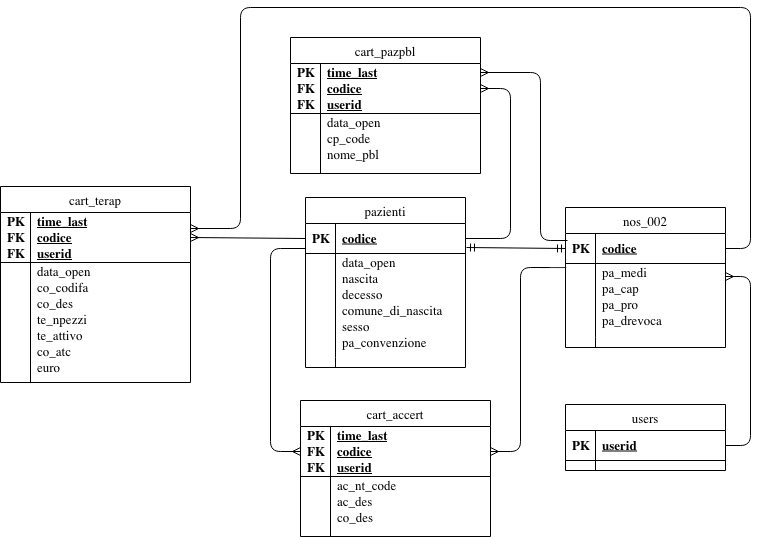
\includegraphics[scale=0.6]{immagini/er.png}
\end{figure}

 
\chapter{Information loss} 
This chapter aims to give a qualitative assessment of the whole database through an initial analysis, giving an overall idea on how impactful is the progressive information loss. 

After assessing the correctness and completeness of records, some fields will be eventually excluded from the analysis, while others that cannot be removed will have a major impact on the results.

Having missing fields, particularly in the process of joining tables, can lead to a \textbf{cumulative augmentation} of the information loss: empty data such as the patient date of birth or gender will cause the deletion of the entire patient, in case analytics is centred on pathologies by age or gender.

Joining is in fact an operation which requires \textit{all fields of reference to be present}, combining entries of the selected tables.

\section{General overview}
Before starting running queries, there are some aspects to consider involving issues which sometimes cannot be addressed just with database interrogations:
\begin{enumerate}
	\item The geographic information is sometimes imprecise and hard to comprehend, since it consists in text fields;
	\item Some diagnoses descriptions don't match with the corresponding ICD-9 code;
	\item A consistent amount of missing data is originated in case a general practitioner doesn't prescribe anything but makes other operations (medical certificates, examinations and such);
	\item Hospital prescriptions are missing;
	\item Some medicines are given over the counter without requiring a prescription, therefore there is no entry in the DB;
	\item General practitioners might prescribe a medicine to a different patient than the one who has the pathology (relatives, friends, \dots);
	\item There is inappropriate prescribing, antibiotic resistance, misuse or over-use of medicines;
	\item A patient can change doctor, so the approach to the same disease may vary.
\end{enumerate}

Furthermore, there have been noticed some common instances of incorrect data:
\begin{itemize}
	\item Some dates don't fall in the acceptable range (e.g.\ 1999, 2034, \dots):
	\begin{itemize}
		\item A date is considered wrong if it falls before 01-01-2000 or after 10-01-2018;
	\end{itemize}
	\item A consistent amount of fields are empty or null.
\end{itemize}

It is important to remember that some records might be affected by more than one incorrect field, therefore when calculating total information loss it is essential to intersect different subsets, to see which records they have in common, instead of just summing the numbers of corrupted rows.

Overall, the loss on single records is not a relevant issue since the total amount of rows allows safe removal, yet the cumulative augmentation (funnel analysis) gives a progressive deletion of information.

\section{Information loss on records}

\subsection{\textit{patients} and \textit{patient\_doctors} (1 million of tuples)}
\subsubsection{Summary}
Both tables contain similar data related to patients, with a $1 : 1$ correspondence between primary keys, therefore joining is an elementary operation and there is no information loss.

\begin{itemize}
	\item Patients with null or empty gender: 2 752 $\rightarrow 0.27\%$;
	\item Patients with gender different from M and F: 54 $\rightarrow 0.005\%$;
	\item Patients with beginning of the patient-doctor relationship outside the accepted range: 226 858 $\rightarrow 22.33\%$;
	\item Patients with null province: 99 981 $\rightarrow 9.84\%$.
\end{itemize}

A subset of patients is creating through an auxiliary view to highlight the final progressive data loss compared to the original tables, joining \textit{patients} and \textit{patients\_doctors} according to those constraints:
\begin{enumerate}
	\item Join on equal patient code (\textit{id});
	\item Not null date of birth;
	\item Dates between 2000 and 2018;
	\item Existing and not null gender;
	\item Existing and not null province.
\end{enumerate}

The total rows respecting all those constraints are 713 352, so approximatively 300 000 tuples (patients) have been deleted. 

This result implies that during analysis there will be at least $\nicefrac{1}{3}$ of the data which is going to be removed due to incompleteness and inaccuracy: not considering patients will imply deleting their diagnoses and prescriptions as well.

A waffle chart is shown on figure \ref{waffle}, highlighting the total tuples and the impact of every restriction, standardised on a scale from 1 to 100:
\begin{figure}[h]
	\centering
	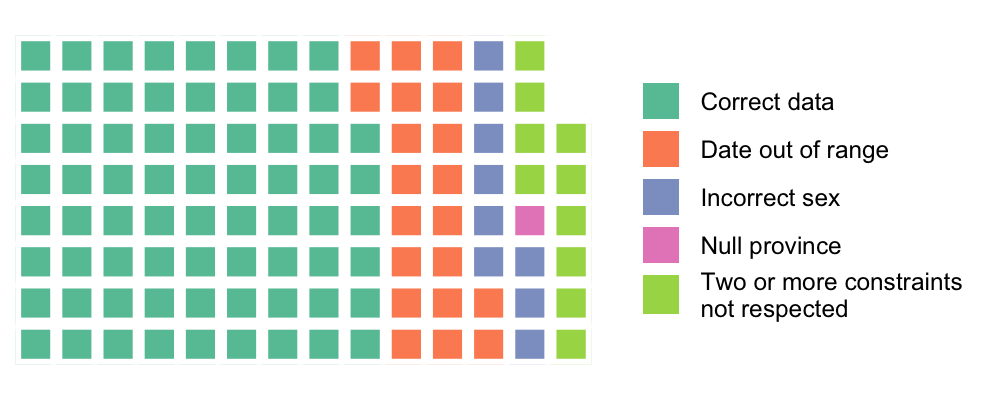
\includegraphics[scale=0.45]{../plots/patients-waffle.png}
	\caption{\small Information loss on patients, waffle plot}
	\label{waffle}
\end{figure}

There are no null provinces and birthdates. The bigger impact is caused by dates falling outside the acceptable range, meaning patients started treatment with their general practitioner earlier than 2000.

\subsection{\textit{diagnoses} (15 millions of tuples)}
\subsubsection{ICD-9}
An ICD-9 code is correct if it is present in the official ICD-9 database\cite{icd9}. General practitioners may use different formats and notations, so before removing codes each one has been subject to preprocessing and parsing.

An ICD-9 code is considered wrong if there is no match in the official DB after any of those transformations:
\begin{enumerate}
	\item Removal of the dot;
	\item Addition of 0 at the beginning;
	\item Addition of 0 at the end;
	\item Removal of the last 0.
\end{enumerate}

There are 76 distinct incorrect ICD-9 codes, a negligible amount considering the total records consisting in 9 895 distinct codes.

\subsubsection{Summary}
\begin{itemize}
	\item Incorrect ICD-9 codes: $76 \rightarrow 0.0005\%$;
	\item Null or empty ICD-9 codes: 2 103 169 $\rightarrow 13.02\%$;
	\item Null or empty descriptions: 656 067 $\rightarrow 4.24\%$;
	\item Dates out of range: 807 985 $\rightarrow 5.23\%$.
\end{itemize}

Empty descriptions almost always correspond to empty ICD-9 codes, therefore the total information loss on descriptions is absorbed by null codes, resulting in the same 13.02\% united percentage.

\subsection{\textit{prescriptions} (118 millions of tuples)}
\subsubsection{ATC code}
The ATC code, unlike ICD-9, has a univocal format (a numeric string of 7 digits), and no parsing is needed. All the codes have been checked with the ontologies in a well-known biology portal\cite{atc}, and an ATC is considered incorrect if there is no match.

There are 1 750 292 non-existent codes, which are caused by:
\begin{enumerate}
	\item Alteration of the codes within the years without updating the database;
	\item Single prescriptions indexed using the superclass code;
	\item Codes only recognised by local pharmacies.
\end{enumerate}

The latter is the most common reason: there are up to 90 000 occurrences of a single unofficial code. Those numbers, despite being high, are not majorly impacting results, considering the total amount of 118 millions of records.

\subsubsection{Summary}
\begin{itemize}
	\item Incorrect ATC codes: 1 750 292 $\rightarrow 1.47\%$;
	\item Null or empty ATC codes: 1 577 749 $\rightarrow 1.33\%$;
	\item Null or empty AIC codes: 1 310 719 $\rightarrow 1.1\%$;
	\item Null or empty descriptions: 101 248 410 $\rightarrow 85.28\%$;
	\item Dates out of range: 3 472 119 $\rightarrow 2.92\%$.
\end{itemize}

Clearly, the prescription description is not a field which can be used for reliable analytics since empty values prevail.

The field \textit{pieces} (number of boxes) might be useful to check for appropriate prescribing, but since the field is a string it requires casting and parsing to integer, and it could be more relevant to focus on prescription patterns.

\section{Total information loss}
Overall, total information loss is shown according by its belonging table. 

\begin{table}[!htb]
	
	\centering
	\begin{minipage}[c]{0.4\linewidth}
				\begin{tabular}{c|c|c}
				\textbf{Table} & \textbf{Records} & \textbf{Percentage} \\
				\hline
				\textit{patients} & 302 266 & 29\% \\
				\hline
				\textit{diagnoses} & 2 403 202 & 15.5\% \\
				\hline
				\textit{prescriptions} & 5 560 191 & 4.7\& \\
			\end{tabular}
	\end{minipage}
	\qquad
	\begin{minipage}[c]{0.4\linewidth}
		\qquad
		\centering
		$\rightarrow$
		\qquad
		\begin{tabular}{c}
			\textbf{Usable records} \\
			\hline
			713 352 \\
			\hline
			13 056 997 \\
			\hline
			113 156 212 \\
		\end{tabular}
		
	\end{minipage}
	\caption{\small Information loss summary}
\end{table}



The aggregated results are not final: each single output from interrogations will be influenced by all the different invalid fields (i.\ e. a patient could have all correct data yet a missing prescription AIC), creating a progressive deletion effect.

Overall, percentages do not compose the majority of tuples, since tables have magnitude order of millions.

 
\chapter{Global analytics}
This chapter concerns global analytics, used to have an initial view on the real value of the data: goals include understanding what kind of information can be extracted and setting practical fields of interest to make deeper research.

The methodology consists in the application of \textbf{exploratory analysis} and \textbf{descriptive statistics} on the existing dataset.

To have a general idea, the considered approach involves the \textit{whole dataset}: all the available information is included, consisting in the entire time range of 18 years and the totality of patients with related records. Missing or incorrect data is then removed, without imposing additional constraints.

Analysis is performed using:
\begin{itemize}
	\item Diagnoses;
	\item Prescriptions;
	\item Patients' phenotype.
\end{itemize}

Performed operations are simple, such as aggregating, ranking and counting, to avoid high computational costs while obtaining clear and comparable results.

Prescriptions are additionally grouped and measured along with diagnoses, to identify eventual linkage between most popular ones, and focus on discrepancies.

The main purpose of global analytics is highlighting unusual patterns and cross-checking information with external studies, confirming anomalies or restricting the field to existing areas of concern.

\section{Most frequent diseases}
Selection of a subset of diseases is possible after preliminary analysis, of which the most immediate regards frequent appearances in the database. 

There are 9 895 distinct ICD-9 in the \textit{diagnoses} table: of those, the 10 most popular ones in terms of count get selected and shown in table \ref{freqdiagn}.

\begin{table}[h]
	\centering
	\begin{tabular}{c|c|c|c}
		\textbf{\#} & \textbf{ICD-9} & \textbf{Count} & \textbf{Description} \\
		\hline
		1 & 799.9 & 441 131 & Other unspecified cause of morbidity* \\
		\hline
		2 & 401.9 & 305 476 & Unspecified essential hypertension \\
		\hline
		3 & 462 & 301 575 & Acute pharyngitis \\
		\hline
		4 & 521.0 & 274 624 & Dental caries \\
		\hline
		5 & 595.9 & 226 428 & Cystitis, unspecified \\
		\hline
		6 & 464.1 & 221 803 & Acute tracheitis \\
		\hline
		7 & 466.0 & 200 408 & Acute bronchitis \\
		\hline
		8 & 780.7 & 183 721 & Malaise and fatigue \\
		\hline
		9 & 530.81 & 182 897 & Esophageal reflux \\
		\hline
		10 & 724.2 & 176 921 & Lumbago
	\end{tabular}
	\caption{\small Most frequent diseases in 18 years}
	\label{freqdiagn}
\end{table}

The most common ICD-9 (*full name: other unknown or unspecified cause of morbidity and mortality) corresponds to a generic unspecified disease, therefore cannot be subject of detailed analysis.

Other diseases vary through chronic and not, different interested age ranges and different organs of the body: further information can be obtained imposing additional constraints on classification.

\subsection{Most frequent diseases based on age}
Since some diseases are likely to appear within specific ages, patients are grouped into \textbf{ranges} and the most common ICD-9 are counted based on the difference between birthdate and prescription date.

\subsubsection{Age ranges}
The classification method follows \textit{international standards} by United Nations\cite{age}, developed on the basis of existing national practices and recommendations concerning age.

Health classification, in particular, identifies the following ranges to the third level of detail:
\begin{enumerate}
	\item Less than 1 year of age;
	\item 1-14 years of age;
	\item 15-24 years of age;
	\item 25-44 years of age;
	\item 45-64 years of age;
	\item 65+ years of age.
\end{enumerate}

Since the available data concerns general practitioners and not paediatricians, although patients in the younger ages are present there is no warranty of completeness of the doctor-patient relationship, therefore the first two ranges have to be removed.

\subsubsection{Results}
The most common diagnosis for each age range is:
\begin{table}[h]
	\centering
	\begin{tabular}{c|c|c|c}
		\textbf{Range} & ICD-9 & \textbf{Patients} & \textbf{Description} \\
		\hline
		3 & 462 & 49 096 & Acute pharyngitis \\
		\hline
		4 & 799.9 & 119 265 & Other unspecified cause of morbidity \\
		\hline
		5 & 401.9 & 140 510 & Unspecified essential hypertension \\
		\hline
		6 & 401.9 & 123 031 & Unspecified essential hypertension \\
	\end{tabular}
	\caption{\small Most frequent diagnosis for age range}
\end{table}

Since range 4 (25-44) has an unspecified disease as the most common, the 2$^{\text{nd}}$ and 3$^{\text{rd}}$ results are listed:
\begin{enumerate}
	\item 462, 97 040 patients, acute pharyngitis;
	\item 521.0, 83 948 patients, dental caries.
\end{enumerate}
Hypertension is more common among older patients, while young adults are mostly affected by pharyngitis and caries.

Overall, the most popular diagnoses according to age reflect the general rankings.

\subsection{Most frequent diseases based on gender}
Since the database contains more female patients than males, it is expected to have a gap between amounts of diagnoses.

The most frequent diagnoses are however \textbf{unrelated} to gender: there are no relevant differences implying a kind of patients is most likely subject to a disease in the considered subset.

Analytics regarding gender have to be performed choosing a different batch of illnesses, taking the ones which are proven to affect one gender rather than the other.

\subsection{Most common diagnoses based on ICD-9 class}
Making ranks from data on a general level is useful to identify most common diagnoses overall, yet only a limited part of all diseases is taken into account.

Information is sliced only according to aggregated total value, without additional considerations and therefore excluding a wide part of the totality.

Since ICD-9 classification divides diagnoses in \textbf{classes} according to the interested part of the body, extracting the most common illness according to its class allows a better understanding of how important is each group and its \textbf{influence} or relation to the prescriptions. Data can be therefore used to make comparisons.

The whole span of 18 years is used to obtain results, having removed records subject to progressive information loss and incompleteness.

ICD-9 analysis show:
\begin{center}
	\begin{table}[h]
		\makebox[\textwidth][c]{
	\begin{tabular}{c|c|c}
		\textbf{Description} & \textbf{Diagnoses} & \textbf{Count} \\
		\hline
		Infectious and parasitic diseases & Herpes zoster & 28 202 \\
		\hline
		Neoplasms & Benign neoplasm of skin & 41 725 \\
		\hline
		Endocrine and metabolic diseases & Pure hypercholesterolemia & 54 935 \\
		\hline
		Blood and blood-forming organs & Anaemia, unspecified & 71 689 \\
		\hline
		Mental disorders & Dysthymic disturb & 43 303 \\
		\hline
		Nervous system & Acute otitis media & 65 776 \\
		\hline
		Circulatory system & Unspecified essential hypertension & 204 995 \\
		\hline
		Respiratory system & Acute pharyngitis & 212 704 \\
		\hline
		Digestive system & Dental caries & 186 540 \\
		\hline
		Genitourinary system & Cystitis, unspecified & 157 684 \\
		\hline
		Pregnancy and childbirth & Caesarean delivery & 3 144 \\
		\hline
		Diseases of the skin & Dermatitis, unspecified & 93 178 \\
		\hline
		Musculoskeletal system & Lumbago & 116 289 \\
		\hline
		Congenital anomalies & Spondylolisthesis & 883 \\
		\hline
		Conditions in the perinatal period & Subdural and cerebral hemorrhage & 587 \\
		\hline
		Symptoms, signs & Other unspecified cause of morbidity & 262 867 \\
		\hline
		Injury and poisoning & Allergy, unspecified & 74 773 \\
		\hline
		External causes of injury & Pregnant state, incidental & 56 169 \\
	\end{tabular}}
	\caption{\small Most popular diagnoses for ICD-9 class}
\end{table}
\end{center}

Number of prescriptions varies from less than 1 000 to more than 250 000, showing the discrepancy of amount of diagnoses among different classes.

Results reflect general analytics, giving additional insight on other categories having consistent values yet not so high to enter the top rankings, such as dermatitis, anaemia and otitis. 

\section{Chronic illnesses}
A chronic illness is defined as \textit{a disease or condition that usually lasts for 3 months or longer and may get worse over time}\footnote{\href{https://www.cancer.gov/publications/dictionaries/cancer-terms/def/chronic-disease}{Cancer.gov definition}}. They can usually be controlled but not cured.

The major limitation of the database is the lacking of fields representing chronic patients, since illnesses can last any amount of time yet be diagnosed only once, therefore counting and ranking does not give relevant information.

Even identifying a subset of chronic patients based on amount of prescriptions or phenotypes would not result in consistent outcomes, because popular diseases such as hypertension or pharyngitis are spread among all patients and a common reason for periodic visits of the general practitioner.

A patient living with a chronic disease can, in fact, have episodes of sporadic disturbs, therefore there is not a clear distinction between diagnoses and illnesses.

According to researches on chronic diseases in Italy, they tend to occur in older adults, aged 45 or more: the total patients of the dataset falling in this category in 2018 is more than half, 625 309.

Some diffused chronic illnesses are:
\begin{itemize}
	\item Hypertension, with 305 476 diagnoses (almost half of the older adult patients);
	\item Arthritis, with 14 110 diagnoses;
	\item Allergy, with 100 744 diagnoses;
	\item Osteoporosis, with 141 671 diagnoses;
	\item Chronic bronchitis, with 70 537 diagnoses (unrelated to bronchitis);
	\item Asthma, with 121 252 diagnoses;
	\item Crohn's disease, with 859 diagnoses;
	\item Fibromyalgia, with 5 818 diagnoses;
	\item Arrhythmia, with 21 394 diagnoses;
	\item Tumour (all, ICD-9 codes 140-239), 288 659 cases.
\end{itemize}

Although there is a chance that the same disease gets diagnosed more than once to the same patient, values are still high compared to 1 million of patients.

\section{Gender-influenced diseases}
Analytics on most frequent diagnoses according to patient's gender do not show additional relevant information, hence outcomes cannot be obtained using popularity as measure. Prescriptions do not vary either, since their nature is preventive and not curative.

Gender-related diseases might not require a considerable amount of visits of the general practitioner, because either of their chronic aspect or their brief duration.

However, there are important \textit{biological and behavioural differences} between categories. They affect manifestation, epidemiology and pathophysiology of many widespread diseases and the approach to health care. 

Since gender affects a wide range of physiological functions, it has an impact on a wide range of diseases including those of the \textbf{cardiovascular}, pulmonary and autoimmune systems, as well as diseases involving gastroenterology, hepatology, nephrology, endocrinology, haematology and neurology\cite{gender}.

Those differences should reflect on the existing data, showing discrepancies between the number of diagnoses for males and females considering the same disease. To verify the hypothesis, a subset of ICD-9 is selected based on external research, and controls are performed.

It is important to consider that female patients are about 4\% more than males.

\begin{table}[h]
	\centering
	\begin{tabular}{c|c|c}
		\textbf{Description} & \textbf{Diagnoses to males} & \textbf{Diagnoses to females} \\
		\hline
		Cystitis (all) & 59 276 & 173 556 \\
		\hline
		Major depression & 1 141 & 1 483 \\
		\hline
		Anxiety states & 13 926 & 23 455 \\
		\hline
		Substance abuse & 1 054 & 142 \\
		\hline
		Erectile dysfunction & 3 944 & 75 \\
		\hline 
		Osteoporosis & 10 129 & 82 655 \\
		\hline
		Anaemia, unspecified & 20 426 & 51 318 \\
		\hline
		Myocardial infarction & 3 672 & 1 399 \\
	\end{tabular}
	\caption{\small Diseases counts based on gender}
\end{table}

Some categories such as drug abuse include all ICD-9 subsets because of their sparsity, while most common illnesses are counted according to specific typologies to avoid dispersion of information.

It is clear that the selected diseases affect a specific gender than the other: females are likely to get cystitis, anxiety, osteoporosis and anaemia, while males are most subject to substance abuse and erectile dysfunction.

The 75 diagnoses of erectile dysfunction to women are a bright example of wrong diagnosing, and are described as ``decrease of sexual desire'' or even ``frigidity''. Those records have to be excluded from analysis of results, showing information loss cannot always be predicted.

Heart attack is an interesting field to look deeper into: researches show difference of signs between women and men, therefore the bigger number of male diagnoses might be caused by females misinterpreting symptoms. 

Overall, studies related to Campania comply with available information on how diseases affect distinct genders.

\section[Most common prescriptions]{Most common prescriptions based on ATC class}
The purpose of analysing most common prescriptions is to highlight similarities between diseases, and verify whether popular products changed within the past year.

The considered time range is 16 years, divided in spans of 8: 2002-2009 and 2010-2017, to have two comparable pictures of data.

Analytics is performed on the first level of each ATC class, and after extracting each pharmaceutical product, its usage is linked with the most common diagnoses, to understand eventual mutual relationships and connections.

The most common ATC codes for category are counted according to their category (table 6.5).
\begin{center}
	\begin{table}[h]
		\makebox[\textwidth][c]{
	\begin{tabular}{c|c|c|c|c|c}
		\textbf{Class} & \textbf{Description} & \textbf{ATC '02-'09} &\textbf{ N. '02-'09 }& \textbf{ATC '10-'17} & \textbf{N. '10-'17} \\
		\hline
		A & Metabolism & Omeprazole & 717 559 & Pantoprazole & 2 350 368 \\
		\hline
		B & Blood & Acetylsalicylic acid & 1 661 035 & Acetylsalicylic acid & 1 939 484 \\
		\hline
		C & Cardiovascular & Nitroglycerine & 891 586 & Atorvastatine & 1 379 261 \\
		\hline
		D & Epidermis & Calcipotriol & 45 545 & Calcipotriol & 69 505 \\
		\hline
		G & Urinary system & Tamsulosin & 288 840 & Tamsulosin & 494 191 \\
		\hline
		H & Hormones & Levothyroxine & 706 394 & Levothyroxine & 838 499 \\
		\hline
		J & Infections & Amoxicillin & 870 151 & Amoxicillin & 1 522 031 \\
		\hline
		L & Tumours & Tamoxifen & 36 208 & Methotrexate & 62 324 \\
		\hline
		M & Muscular system & Nimesulide & 1 074 632 & Ketoprofen & 740 165 \\
		\hline
		N & Nervous system & Paroxetine & 177 918 & Escitalopram & 348 080 \\
		\hline
		P & Antiparasitic & Hydroxychloroquine & 27 977 & Hydroxychloroquine & 52 150 \\
		\hline
		R & Respiratory & Beclometasone & 412 688 & Beclometasone & 531 337 \\
		\hline
		S & Sensory organs & Timolol & 162 444 & Timolol & 237 196 \\
		\hline
		V & Various & Oxygen & 103 379 & Oxygen & 246 050 \\
	\end{tabular}}
	\caption{\small Most frequent prescription per AIC class}
\end{table}
\end{center}

\subsection{Comparison of results}

\subsubsection{Alimentary tract and metabolism}
The A class shows some potentially concerning results: values of prescriptions of those drugs have tripled from 2002-2009 to 2010-2017. Omeprazole has been substituted by Pantoprazole as top prescribed, yet its prescriptions grew considerably. Both products are for eophageal reflux, which is one of the most diagnoses diseases.

A brief time series analysis on the original \textit{prescriptions} table helps to visualise the growth of the two medicines:
\begin{figure}[h]
	\centering
	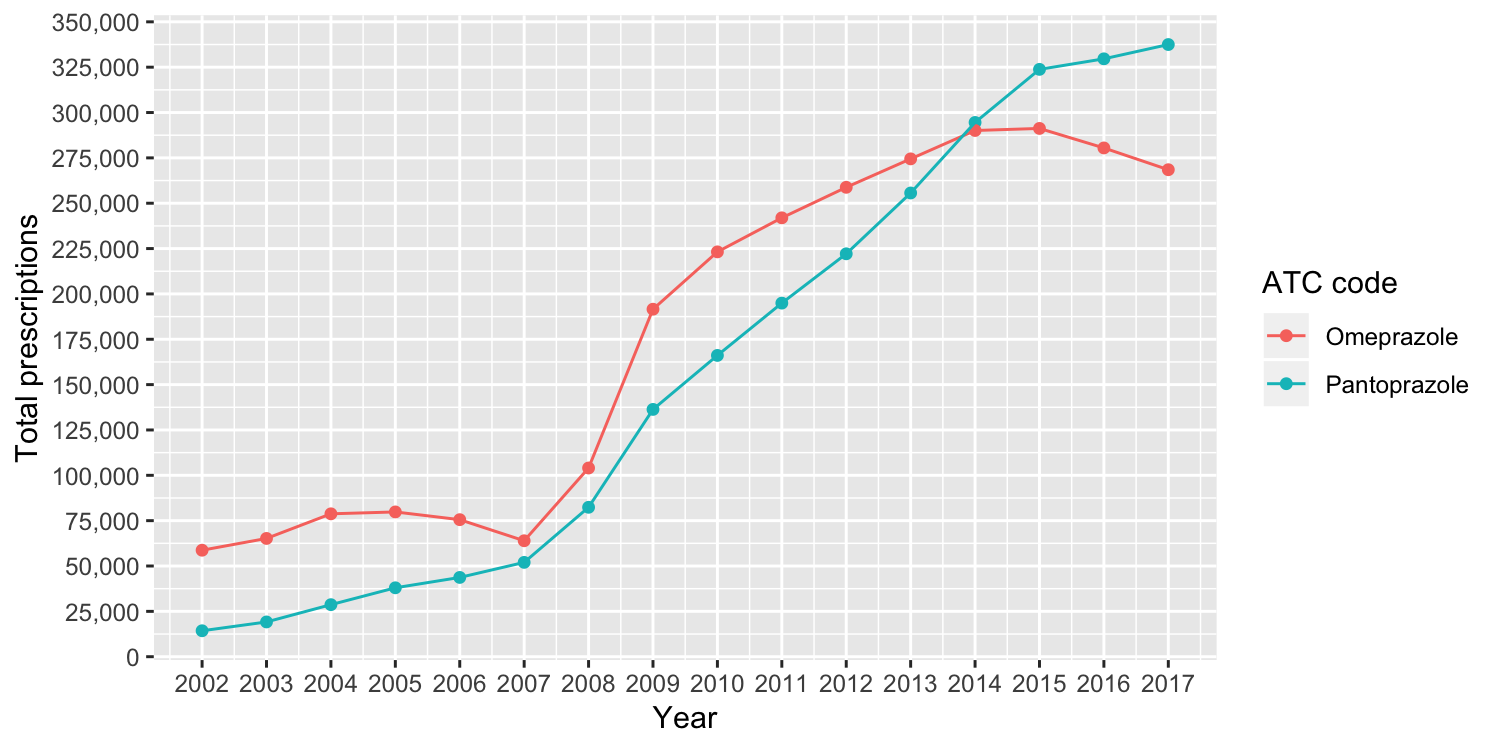
\includegraphics[scale=0.3]{../plots/atc-a-gastro.png}
	\caption{\small Omeprazole and Pantoprazole trends}
\end{figure}

The trend is subject to a drastic change starting from 2007, with a switch of most popular in 2014.

Further examinations confirm that, despite other alimentary tract medicines have lower values, the number of prescriptions of a consistent amount of those is higher than 1 million, yet the raising trend only concerns omeprazole and pantoprazole. 

The hypotheses for changes in patterns are:
\begin{enumerate}
	\item A bigger amount of information falling in the 2010-2017 range;
	\item An effective increase in esophageal reflux and therefore prescriptions related to it.
\end{enumerate}

There are approximatively 18 more millions of tuples overall in 2010-2017, but considering a total amount of 118 millions, the unusual growth cannot be justified by information loss.

Diagnoses of esophageal reflux within years are then counted:
\begin{figure}[h]
	\centering
	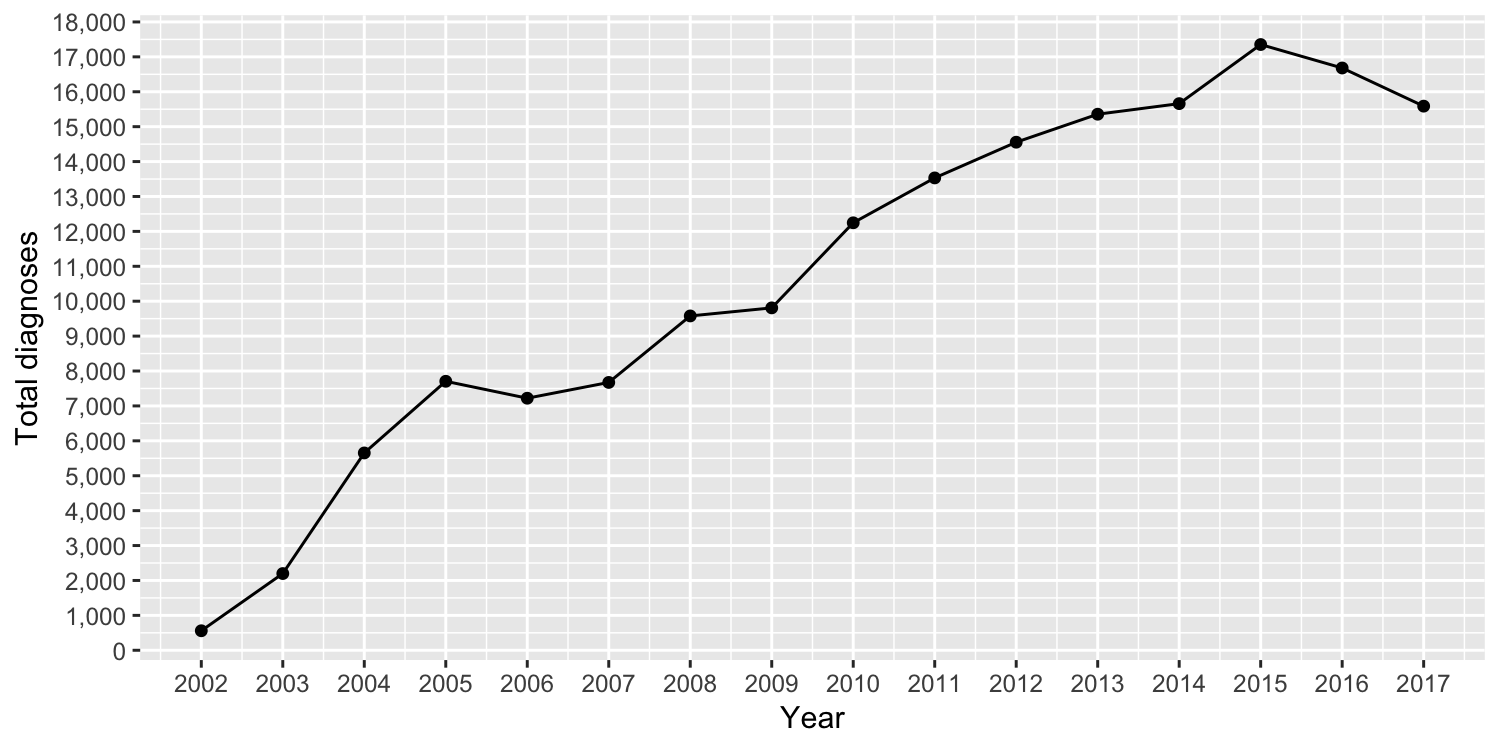
\includegraphics[scale=0.3]{../plots/reflux.png}
	\caption{\small Esophageal reflux trends}
\end{figure}

Values started from less than 1 000 and got to almost 18 000, yet numbers are still too small to explain 300 000 yearly prescriptions. 

Other approaches to have a deeper understanding can involve reconstructing the patients history, or extracting the common diagnoses of patients with a prescription of omeprazole or pantoprazole.

\subsubsection{Blood and blood forming organs}
Blood class has as major product acetylsalicylic acid, which is the active principle of aspirin. This case most likely regards cardio-aspirin, used to prevent and treat heart diseases and as anti-thrombotic.

\subsubsection{Cardiovascular system}
Atorvastatin is the most common medicine in 2010-2017, already confirmed by gender-related analysis. Before 2010, however, the highest-ranked prescriptions was nitroglycerin, followed by amlodipine and simvastatin. 

Numbers suggest a consistent switch of products while dealing with cardiovascular system disease. Values increased, confirming the national issue of heart diseases as principal death cause\cite{ansacuore}.

Those classes of active principle are used for cholesterol control as well, therefore this can have an influence on the prescription trends.

Nitroglycerin lost popularity, probably because of its heavy side effects, unclearness of mechanism or potential danger while interfering with other medicines or defibrillation. 

\subsubsection{Dermatologicals}
Skin medicines aren't subject of relevant mutations: the most popular is still calcipotriol (calcipotriene), a form of vitamin D.

The usage is mainly for psoriasis, which is discordant with the top ranked unspecified dermatitis in the ICD-9 analysis.

There are 30 768 entries in the whole database for ICD-9 codes concerning psoriasis (696.*), approximately $\frac{1}{3}$ respecting to dermatitis and $\frac{1}{4}$ of prescriptions, yet psoriasis is a chronic disease and only gets diagnosed once.

\subsubsection{Genito-urinary system and sex hormones}
Urinary system diseases have as most prescribed drug tamsulosin, for benign prostatic hyperplasia. The most diagnosed issue is cystitis, yet it doesn't usually get treated with a medicine cure.

There are 63 368 cases of prostatic hyperplasia in the whole database, which compared to the $\sim$700 000 total prescriptions doesn't explain such high value. It is not a chronic disease, nor prescribed to women and kids, therefore this phenomenon should be looked further into.

\subsubsection{Systemic hormonal preparations, excluding sex hormones and insulins}
Levothyroxine is one of the most prescribed products in the United States, for hypothyroidism: more than 12\% of the US population is affected by this disease, while in Italy the percentage is around 10\%.

The discrepancy may be due to different lifestyle or lack of diagnoses: in the Campania database there are 29 184 cases in 18 years, which is a small amount compared to the top diagnoses.

\subsubsection{Antiinfectives for systemic use}
Amoxicillin, belonging to the penicillins group, is the most used medicine for infections: its scope covers ear, pharynx, airways, skin, teeth and urinary system infections.

Generally penicillins cover almost the entire amount of prescriptions for infections: this can be related to the high quantity of diagnoses concerning otitis, pharyngitis, laryngitis, bronchitis and tracheitis. 

Number of prescriptions between the two time ranges has doubled, which consists in a starting point to affirm the spread of antibiotic resistance and lack of ethical prescriptions.

\subsubsection{Antineoplastic and immunomodulating agents}
Prescriptions for the antineoplastic category tend to vary: from 2010 there is a prevalence of methotrexate, used to treat tumours, especially leukaemia but also psoriasis, regional enteritis and rheumatoid arthritis.

Previously, the most used product is tamoxifen, for breast cancer. All the other common prescriptions consist in inhibitors, which could mean cases of breast cancer is decreasing.

The database shows 3 805 cases in 2002-2009 and 4 086 in 2010-2017, yet the values are biased because of the bigger amount of information related to the most recent years.

\subsubsection{Musculo-skeletal system}
The popular prescriptions for the muscular system are the same within years, yet their amount drastically changes.

Nimesulide is a nonsteroidal anti-inflammatory drug used for acute pain treatment in orthodontic, rheumatological and gynaecological fields. The medicine has encountered various collateral effects on an European level.

Toxicity and adverse reactions explain the decrease in the number of prescriptions and the switch to Ketoprofene, another nonsteroidal anti-inflammatory drug to treat rheumatological arthritis and osteoarthritis.

\subsubsection{Nervous system}
Powerful antidepressants lead the area of nervous system drugs: although the two products are different in the considered time spans, the class is the same (inhibitors of serotonin receptors).

Prescriptions values are increasing, despite the number of dysthymia diagnoses going from 22 656 to 20 647, therefore other illnesses treated with antidepressant could be spreading (depression, anxiety).

\subsubsection{Antiparasitic products, insecticides and repellents}
Hydroxychloroquine is the only product in this category which is consistently prescribed and passes the 10 000 entries: this is because although it being an antimalarial, it gets used for rheumatological arthritis and lupus.

\subsubsection{Respiratory system}
Different time spans show no relevant differences in the amount of prescriptions of drugs for the respiratory system, yet beclometasone has a detach from all the other medicines (almost double the amount).

\subsubsection{Sensory organs}
Timolol is prescribed for hypertension, one of the most diagnosed diseases overall. There is coherence between diagnoses and prescriptions, yet a difference of approximately 100 000: cases must be increasing.

\subsubsection{Various}
Most common various product is oxygen, having a wide spectrum of uses including cardiac insufficiency, chronic bronchitis and bronchopneumonia: crossing diagnoses happening the same day of this prescription would give an overall idea of the leading diagnoses.

\section{Conclusions}
% fare bene
Overall, data show a general trend of increase of both diagnoses and prescriptions. In most cases, this can be attributed to the presence of more information in the recent years, yet some specific instances raise concerns.

Research could get detailed results through a time series analysis on:
\begin{itemize}
	\item Esophageal reflux and metabolism prescriptions;
	\item Antibiotic resistance;
	\item Tumours and benign hyperplasia. 
\end{itemize}





 % tutto
\chapter{Patient journey}
After the preliminary analysis and deciding the main focus area, there are enough information to begin reconstructing the \textbf{patient journey}. The goal of this process is to highlight changes in \textit{prescription patterns for chronic diseases}, starting from the medical history of patients.

An objective definition of patient journey can be created using the following guidelines:
\begin{enumerate}
	\item Patients with \textbf{complete medical history} for a fixed amount of years;
	\item Records with patient, prescribing GP, diagnosis and prescription on the \textbf{same date};
	\item Only \textbf{first-time }diagnoses and prescriptions considered.
\end{enumerate}

The imposed criteria is very strict: taking diagnoses and prescriptions on the same day means removing \textit{all prescriptions} following the first diagnosis. In other words, all the instances of patients coming back to their GP to renew a prescription for a chronic disease have been deleted.

This can be useful to extract a cohort of patients beginning their treatment, and analyse the variations of first-time prescriptions. It's important to notice that not all doctors may have patients with a new chronic illness.

\section{Imposed criteria}
Aside from the completeness and correctness of the data, there are more restrictions to maintain the consistency:
\begin{itemize}
	\item The prescribing general practitioner mustn't change in the time range;
	\item The patient mustn't be deceased;
	\item There must be a sanitary convention;
	\item The general practitioner must be active.
\end{itemize}

All those constraints can be checked using the related fields in the database: \textit{pa\_drevoca} for interruption of the relationship, \textit{decesso} for death and \textit{pa\_convenzione} for the sanitary convention.

The table \textit{users} contains all the IDs of active general practitioners, so joining it with other tables is enough to remove all the rows with an inactive GP. Data is up to date, but since the patient journey will include 2018 (the focus is on the most recent information) there is no need to check for active GPs in the previous years.

The biggest risk is again the \textbf{loss of information}: the impact of data cleansing is heavy, and the obtained results might not give an insightful prospective.

\section{Initial data cleaning}
An initial data cleaning has been made on the whole database to have a first understanding of the potential information loss.

In this case, having such a big amount of tuples is useful: it's possible to remove a considerable percentage of them without losing generality and still having numerous samples.

Information on the general loss is already available thanks to the specific analysis on each single field, so the shown data cleaning will only consider patients and GPs.

The active general practitioners are \textbf{432}: this result has been retrieved counting the different IDs in \textit{users} (438) and removing the ones that weren't present in \textit{nos\_002} (6).

The following \textit{pie chart} illustrates the data loss on patients according to the criteria defined in the previous section.
\begin{figure}[h]
	\centering
	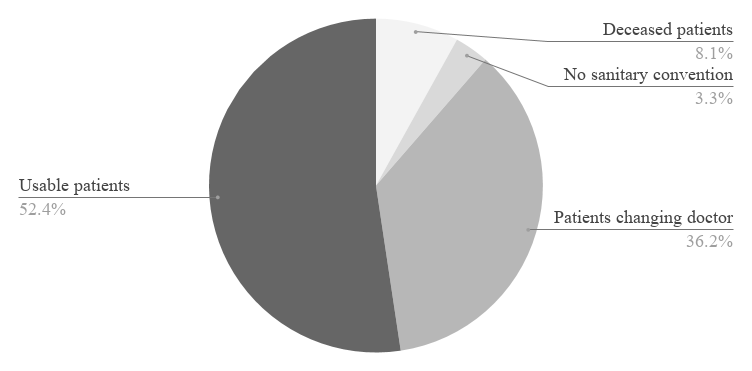
\includegraphics[scale=0.6]{images/pie0018.png}
\end{figure}

About half of patients is going to be lost, due to not respecting the consistency criteria. Starting from a million of records, concrete results are still obtainable.

\section{First approach}
The first approach consists in testing with an \textbf{arbitrary range constraint}: all dates must fall in the span between 2010 and 2018.

The analysis has pure research purposes, to understand the impact of a cut of the dataset in terms of information loss. All the previously introduced criteria must be considered as well, so there must be a continuous doctor-patient relationship between active GPs and non-deceased patients with sanitary conventions.

The outcome is a patient journey table containing data from 2000 to 2018, with a total amount of \textbf{144.618} tuples: this means that there are roughly 150k of first-time diagnosis and prescriptions to patients. 

\subsection{Results breakdown}
Seeing that the starting tables had number of rows in the order of millions, some deeper analysis is necessary to figure out the causes of this huge loss.

The 144.618 complete tuples are composed by:
\begin{itemize}
	\item 27.733 patients;
	\item 422 general practitioners;
	\item 1.381 unique diagnoses;
	\item 904 unique prescriptions.
\end{itemize}

Further causes for those low values can be found counting how many dates would not fall in the considered range. The percentage of records with date earlier than 2010 in each table is:
\begin{itemize}
	\item Patients: 75\%;
	\item Diagnosis: 54,6\%;
	\item Prescriptions: 44,7\%.
\end{itemize}

There is an enormous loss on patients: the possible reason might be that most patients started treatment earlier than 2010, plus diagnosis and relative prescription are in different dates.

8 years is a too wide range to obtain a consistent patient journey, and such information loss isn't negligible: the conclusion of the first approach is that introducing time boundaries is something which needs an accurate control, to avoid missing out most of the data.

\newpage
\section{Second approach}
Since just removing according to the date is an abrupt approach, it's necessary to tune parameters and introduce more detailed constraint, to have a bigger amount of information.

The focus is on the number of prescriptions: given a small range of years, only patients with at least one new prescription are going to be considered. All the previous criteria must be respected, so there must be a continuous doctor-patient relationship between active GPs and non-deceased patients with sanitary conventions.

This methodology allows cluster sampling without having to remove half of the dates: criteria based on the number of prescriptions creates another patient cohort which can be used to accurately select rows from the other tables.

The proposed time range is 2016-2018: pharmaceutical companies generally use the last two years of sales, so picking the last three years gives additional information without compromising the consistency of data.

The outcome is a patient journey consisting of 1.465.005 tuples: almost 10 times the previous result. This leads to two important statements:
\begin{enumerate}
	\item The time range is appropriate, since the number is large enough to make analysis without loss of generality;
	\item The new imposed criterion gives more consistent data and the possibility to build time series.
\end{enumerate}

More cleaning is required to link diagnoses and prescriptions, since there is not a 1:1 correspondence: multiple diagnosis and prescriptions may be associated to the same date. This can be done using a lookup table.

\subsection{Results breakdown}
The 1.665.005 complete tuples are composed by:
\begin{itemize}
	\item 230.381 patients;
	\item 422 general practitioners;
	\item 1.381 unique diagnoses;
	\item 904 unique prescriptions.
\end{itemize}

Only 7\% of the total prescription has been taken in consideration, yet a million and half is still a satisfying amount.

\section{Results comparison}
Comparing the two patient journey outcomes through graphs is a good way to visualize changes and improvements.

\subsection{Changes in data composition}
% todo

\subsection{Improvement on patients information loss}
% todo
A pie chart for data loss on patients in the range 2016-2018 has been made to compare with the previous one.

\begin{figure}[h]
	\centering
	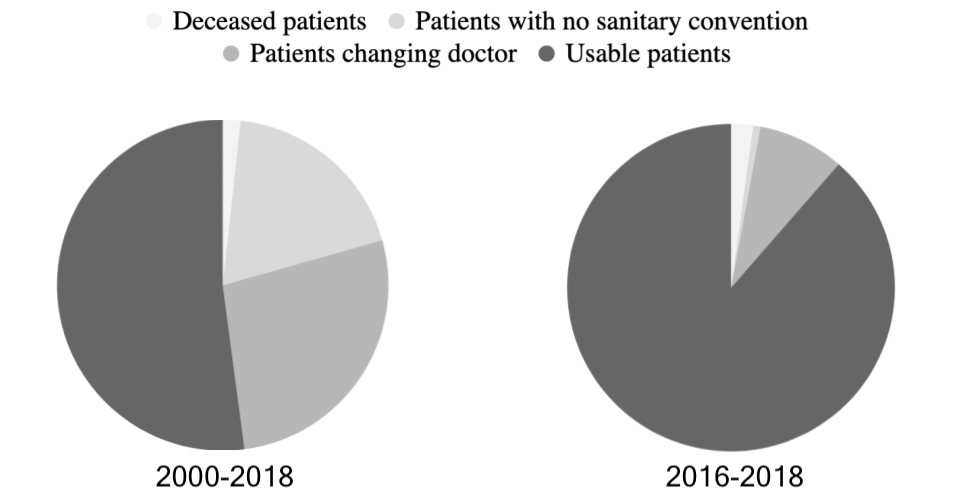
\includegraphics[scale=0.5]{images/pies.png}
\end{figure}

It's easy to see that the number of usable patients has noticeably increased: using a smaller time span reduces the chances of death and change of GP.

\subsection{Funnel graph of patients}
A funnel graph is useful to see how imposing every restriction made the patients number decrease: starting from a million, in the end there only is about $\nicefrac{1}{4}$ of it.








% \chapter{Antibiotic trends analytics}
Having obtained a general analytical view on couples of first-time diagnoses and prescriptions, and cross-checking those results with global trends, the research focusses on antibiotic prescriptions to identify changes of patterns.

Defined time frames in limited temporal windows are selected to make a detailed trajectory analysis related to prescriptive appropriateness compared to antibiotic resistance, without going into details of pathologies.

Such analytics are useful for research, highlighting rising health issues alongside the AIFA reports, and to support pharmaceutical companies using the potentiality of healthcare data. Having information about AICs allows to give a new insight not only on ethical matters, but also on the global market trends.

\section{Identifying antibiotics}
Antibiotics, also known as antibacterials, are medications produced by microorganisms that destroy or slow down the growth of bacteria. They include a range of powerful drugs and are used to treat diseases caused by bacteria. 

A doctor can prescribe a broad-spectrum antibiotic to treat a wide range of infections. A narrow-spectrum antibiotic is only effective against a few types of bacteria. In some cases, a healthcare professional may prescribe to prevent rather than treat an infection, as might be the case before surgery. 
 
 ATC codes related to antibiotics divided by class are:
 \begin{itemize}
 	\item A01AB, A02BD, A07A;
 	\item D01, D06, D07C, D09AA, D10AF;
 	\item G01;
 	\item J, the whole class;
 	\item R02AB;
 	\item S01A, S02A, S03A (removing hormones).
 \end{itemize}

\section{Subset extraction}
The first criteria to impose, considering analytics is going to be made on antibiotic prescriptions, is the actual presence of such. This can be reworded by removing all data related to patients who never had a prescription of an ATC code among the ones previously listed.

There are 794 267 patient with at least one antibiotic prescription in the whole time range (2000-2018), whose total prescriptions consist in 114 044 470 tuples. This implies the remaining 200 000$\sim$ patients only have 4m$\sim$ prescriptions, which is probably justified by a healthier physical state.

Since antibiotics patterns are subject to major changes during years, a big amount of data can be dispersive: pharmaceutical companies make analysis only considering 2-3 years, yet for research purposes an intermediate range is the most informative. A good time span is 10 years, considering most recent ones: since 2018 has to be excluded due to incompleteness, 2008-2017 is the final choice.

Progressive data loss has to be considered, imposing additional constraints of completeness and accuracy. The latest version of the used dataset is a subset of the table prescriptions, with the following restrictions:
\begin{itemize}
	\item AIC corresponding to an antibiotic;
	\item Prescription date between 2008-01-01 and 2017-12-31;
	\item Active general practitioners;
	\item Patients with usable information about sex, date of birth and location.
\end{itemize}

The obtained record set is composed by 8 386 057 tuples, each representing a single prescription.

\section{Global statistics}
Global statistics help to have a general overview of the data, aggregating values to identify most impactful changes and the broad behaviour.

\subsection{Average prescriptions}
The average number of prescriptions has been calculated only considering the number of patients with at least one antibiotic prescription from 2008 onwards (670 634). 

Values are calculated using the R functions \texttt{mean} and \texttt{sd}, only considering the number of patients who received at least one prescription in the determined year.

\begin{center}
	\begin{tabular}{c|c|c}
		Year & Mean & Standard deviation \\
		\hline
		2008 & 2,72 & 2,73 \\
		\hline
		2009 & 2.75 & 2,78 \\
		\hline
		2010 & 2,72 &  2,76 \\
		\hline
		2011 & 2,69 &  2,73 \\
		\hline
		2012 & 2,68 & 2,76 \\
		\hline
		2013 & 2,74 & 2,84 \\
		\hline
		2014 & 2,79 & 2,88 \\
		\hline
		2015 & 2,79 & 2,79 \\
		\hline
		2016 & 2,77 & 2,91 \\
		\hline
		2017 & 2,72 & 2,84 \\
	\end{tabular}
\end{center}

Values show the mean tends to slowly increase, and although there are patients getting up to 30 antibiotic prescriptions each month, the standard deviation is low: the mode both for year and month is 1, so lower values weigh more.

Statistics related to the number of patients with only one antibiotic prescription, making statistics comparing time spans between 2008-2017:
\begin{center}
	\begin{tabular}{c|c|c}
		Interval & Mean & Standard deviation \\
		\hline
		Year & 118 301,4 & 2 831,65 \\
		\hline
		Month & 40 130,83 & 6 004,2 \\
	\end{tabular}
\end{center}

\subsection{Yearly prescriptions}
The number of yearly antibiotic prescriptions is:
\begin{table}[!htb]
	\centering
	\parbox{0.25\textwidth}{
		\begin{footnotesize}
			\begin{tabular}{c|c}
				Year & Antibiotics \\
				\hline
				2008 & 813 337 \\
				\hline
				2009 & 846 067 \\
				\hline
				2010 & 797 472 \\
				\hline
				2011 & 777 582 \\
				\hline
				2012 & 760 280 \\
				\hline
				2013 & 798 320 \\
				\hline
				2014 & 812 594 \\
				\hline
				2015 & 802 323 \\
				\hline
				2016 & 776 756 \\
				\hline
				2017 & 727 723 \\
			\end{tabular}
		\end{footnotesize}
	}
	\qquad
	\begin{minipage}[c]{0.6\textwidth}
		\centering
		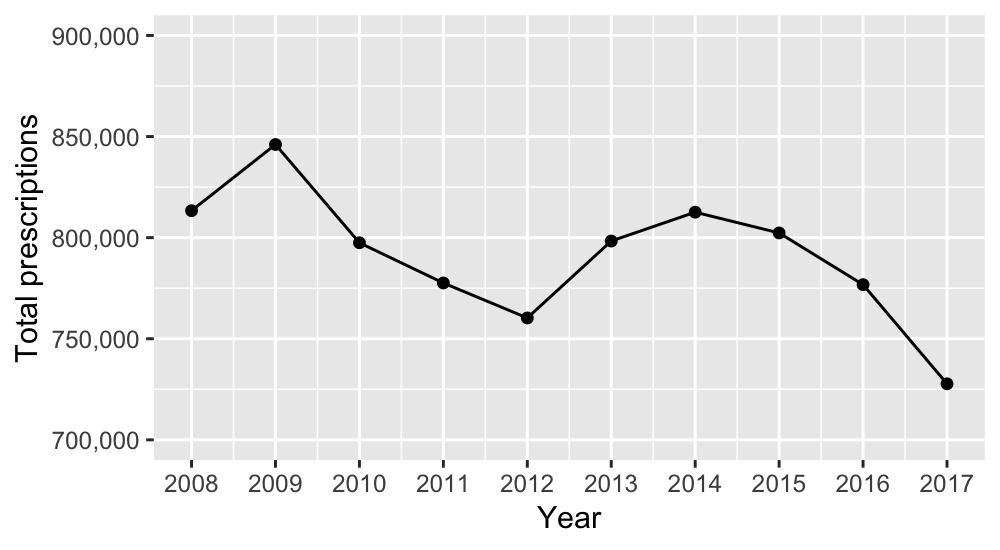
\includegraphics[width=1\textwidth]{../plots/yearly_prescriptions.png}
	\end{minipage}
\end{table}

The 2012 fall might be caused by the substantial decrease of the approved antibiotics by AIFA\cite{calo}, but is noticeable that the number rises starting from 2013 due to antibiotic resistance. 

\subsection{Number of prescriptions trends}
A barplot is the most informative way to visualise trending of number of prescriptions and highlight seasonality. For each month, the amount of patients having the number of prescriptions stated in the x-axis is plotted, using a logarithmic scale.

The scale has been adopted to standardise the quantity of patients having a smaller number of prescriptions (1-2), giving higher bars to larger values.

\begin{figure}[h]
	\centering
	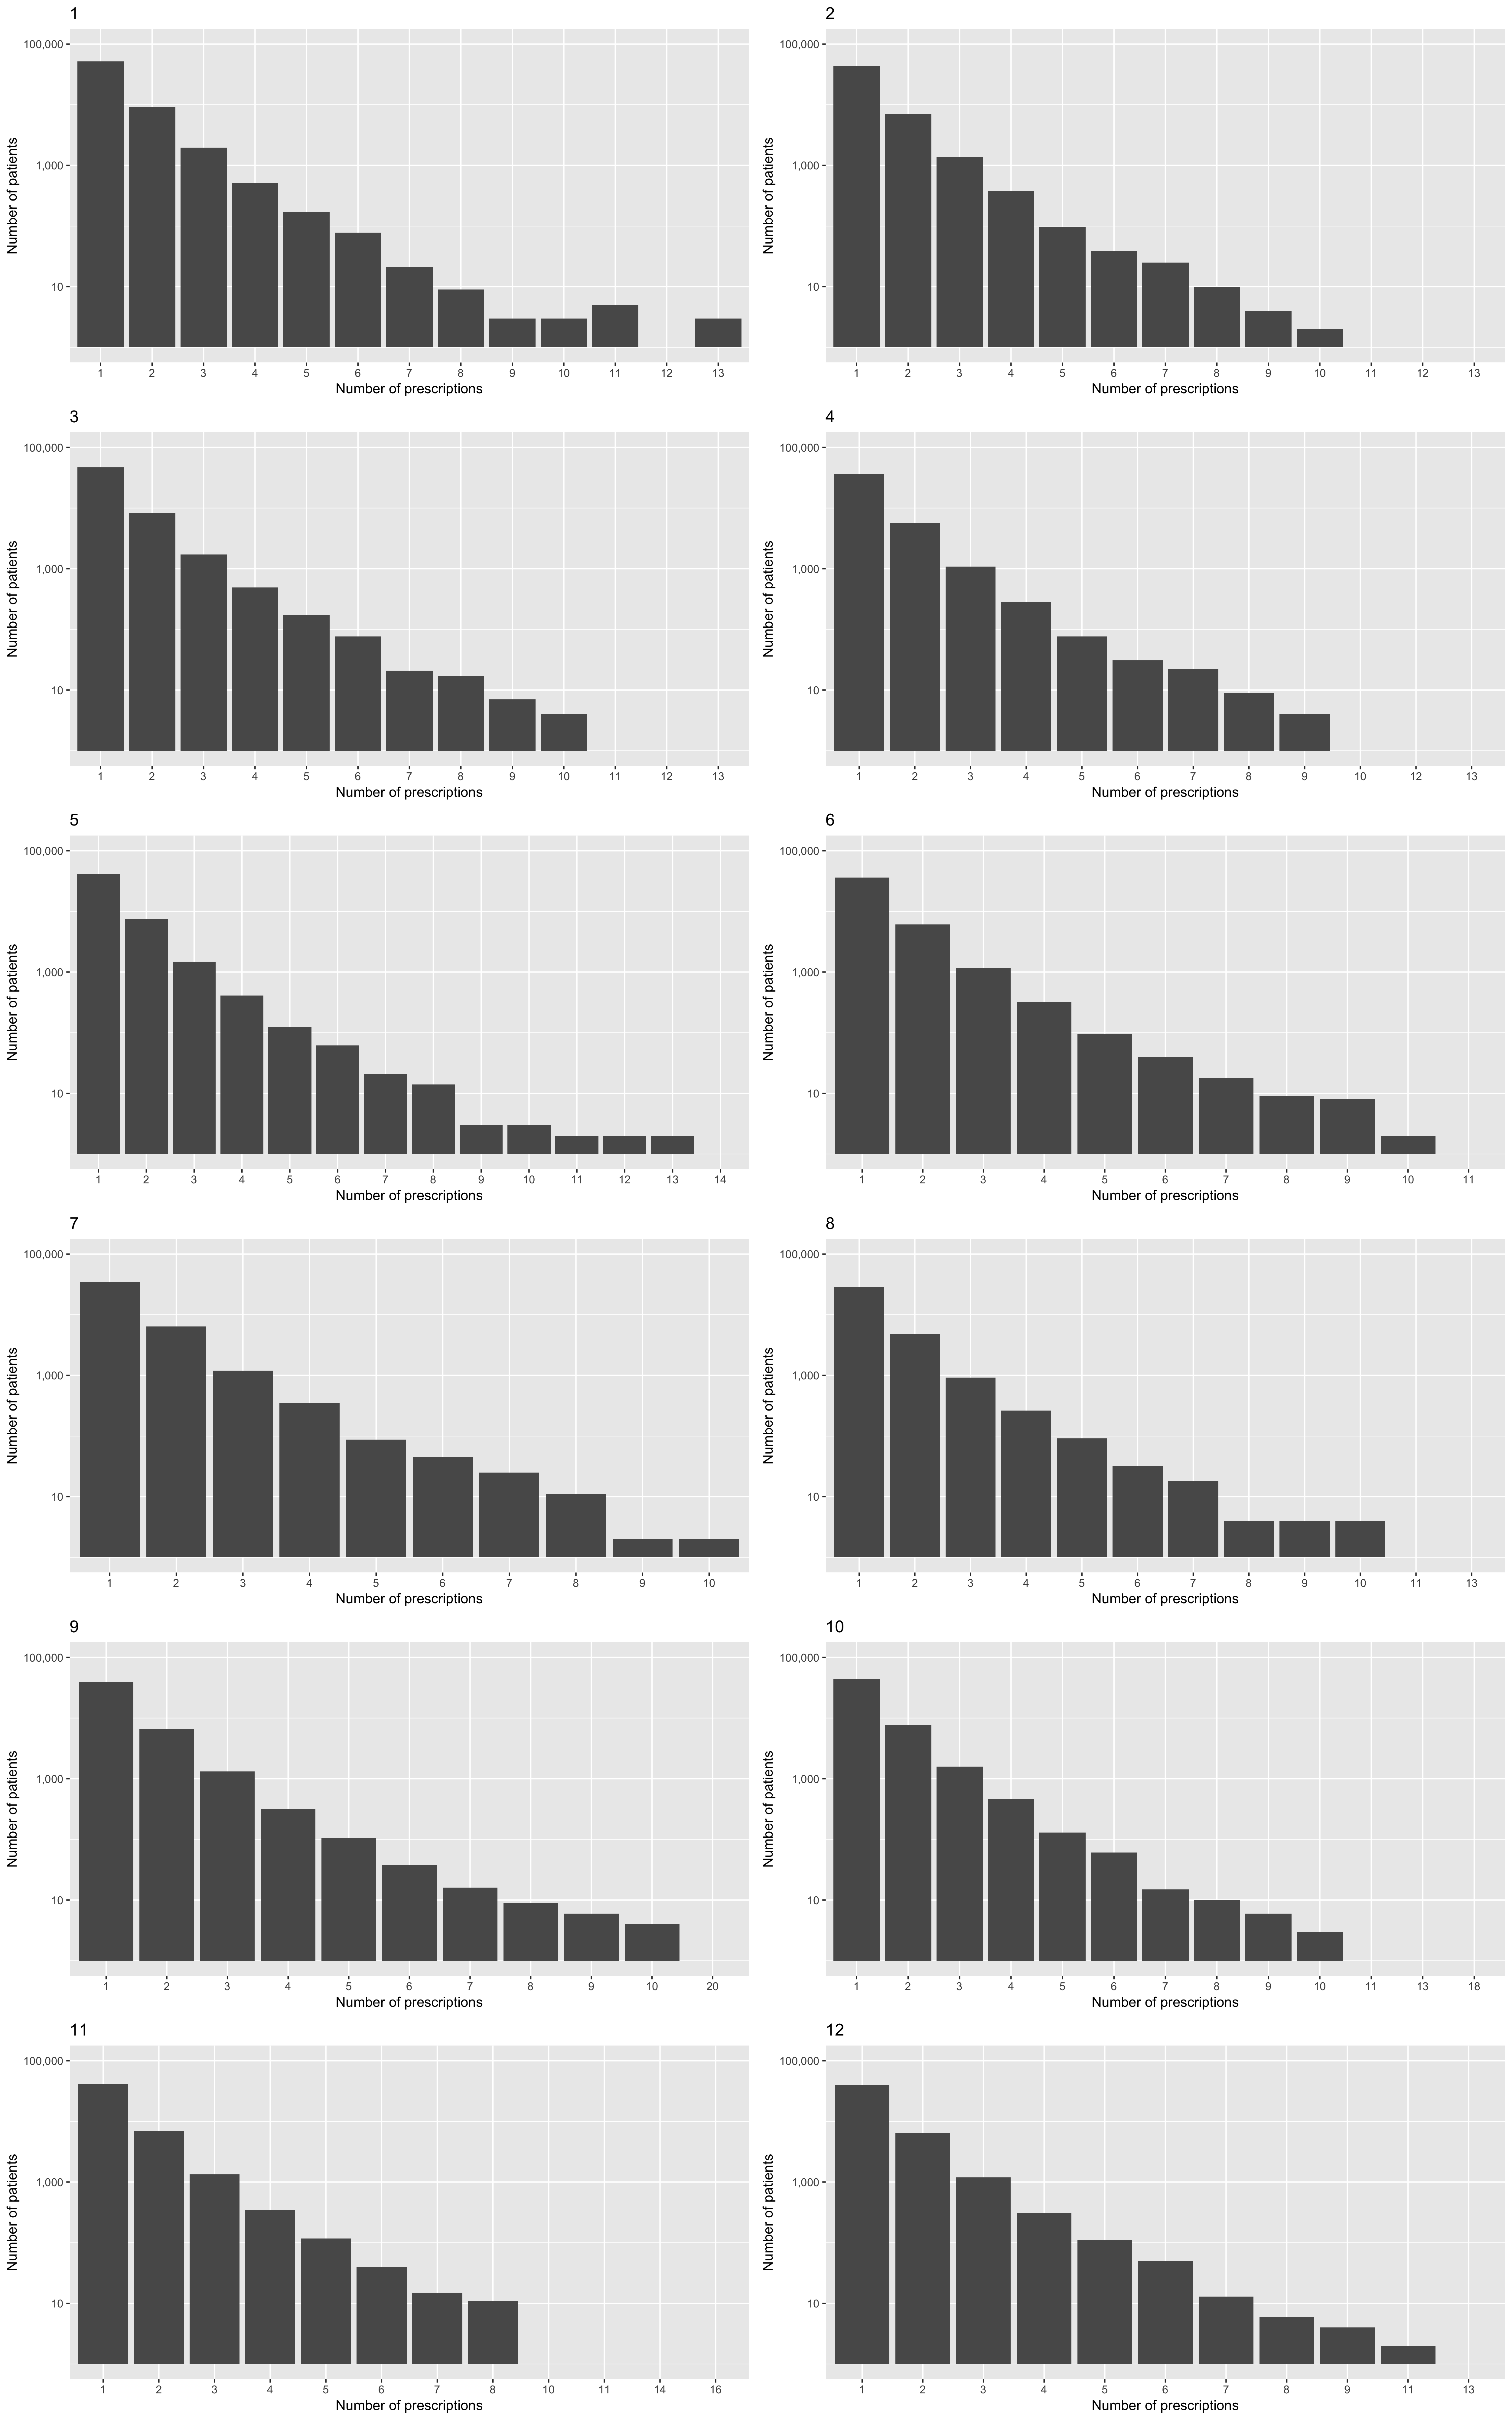
\includegraphics[scale=0.135]{../plots/prescriptions_number-month.png}
\end{figure}

In winter there are more patients having a larger number of prescriptions, while during the summer higher values tend to disappear and even patients with one prescription decrease.

\section{ATC rankings}
For each year and each month, the 3 most common antibiotics are extracted, according to their ATC code. Top 3 changes during the years, hence why there are more than 3 labels in the plots. 
\begin{figure}[h]
	\centering
	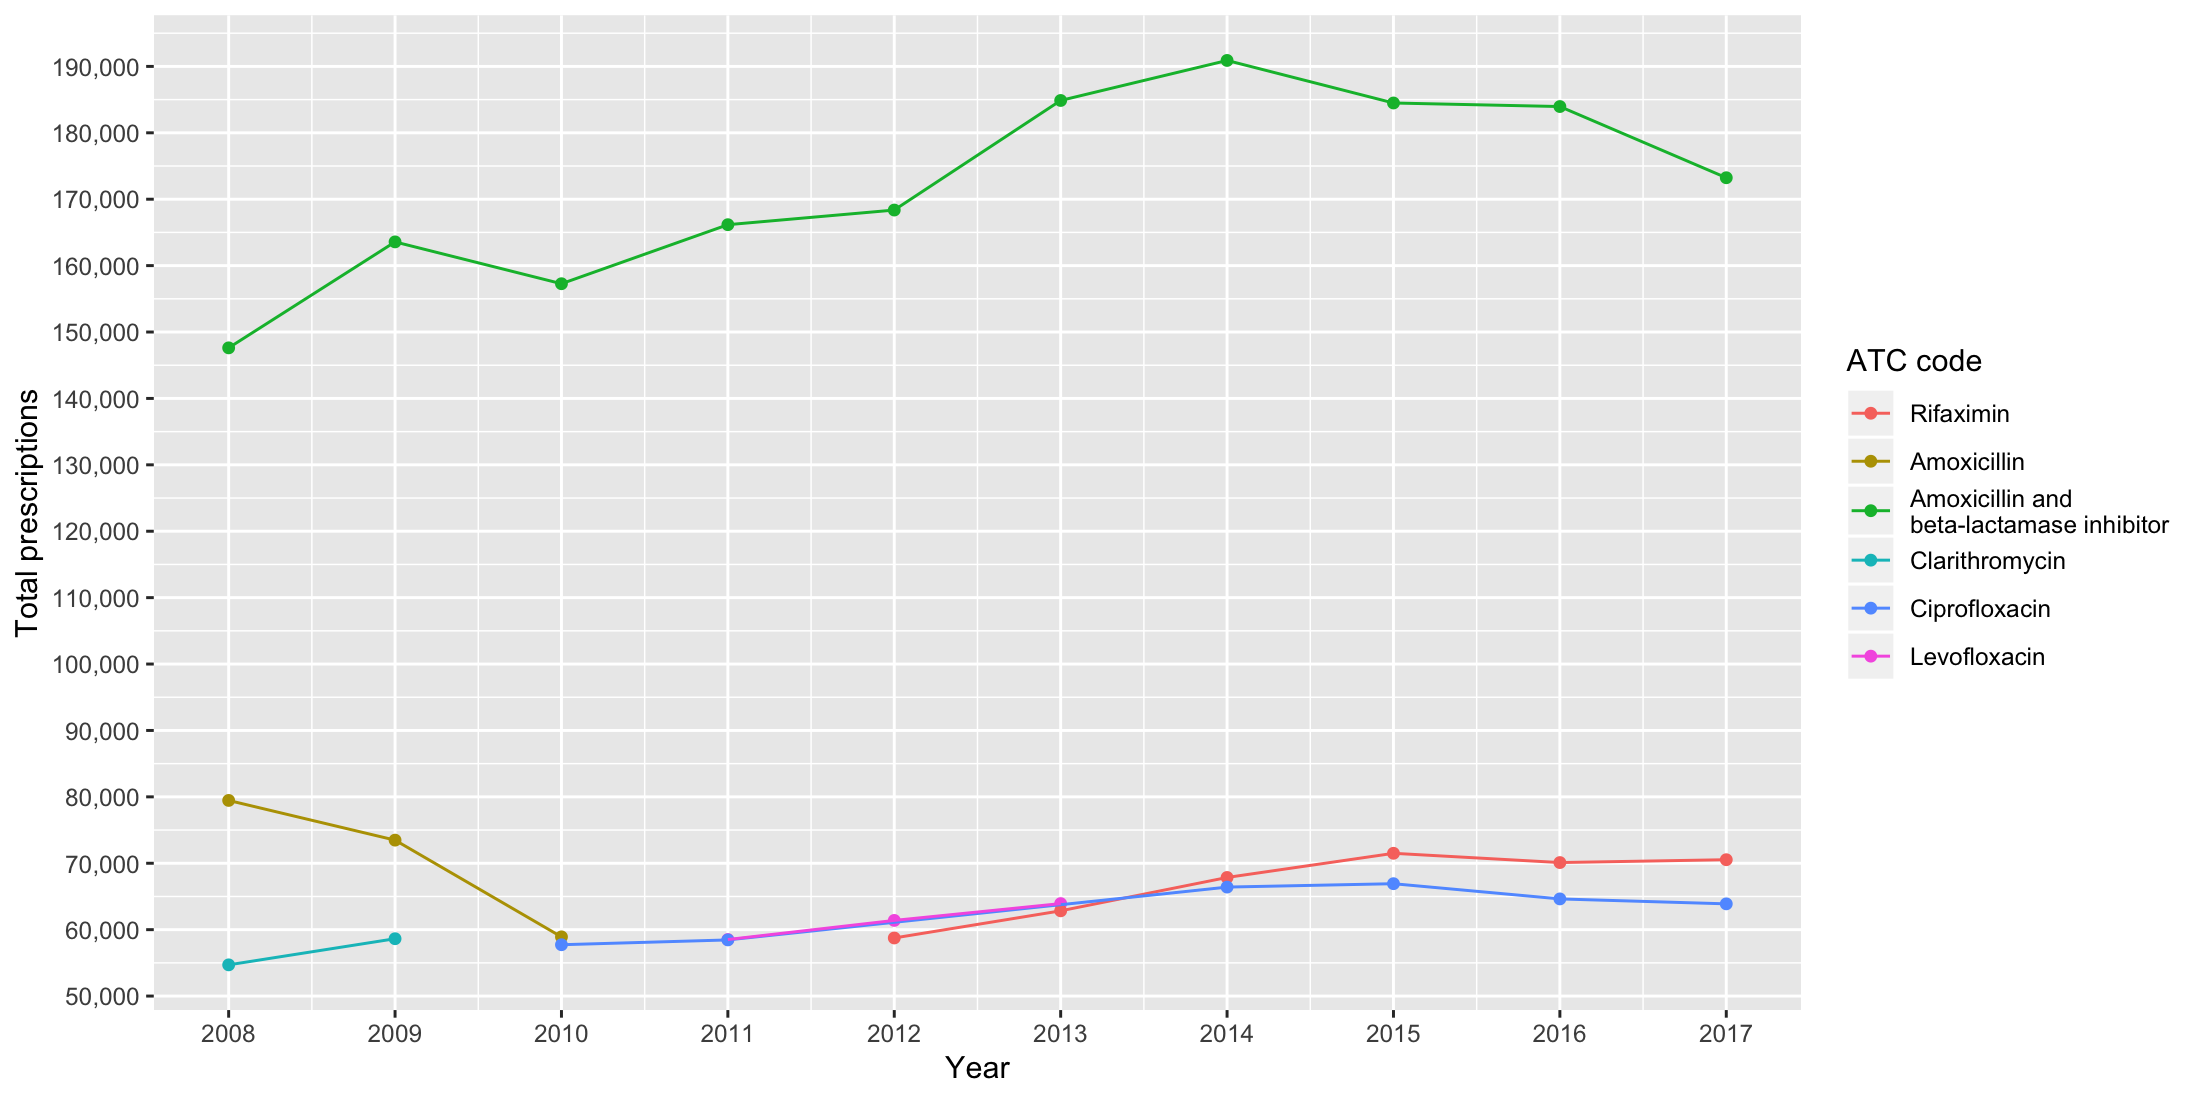
\includegraphics[scale=0.3]{../plots/top_atc-year.png}
\end{figure}

\begin{figure}[h]
	\centering
	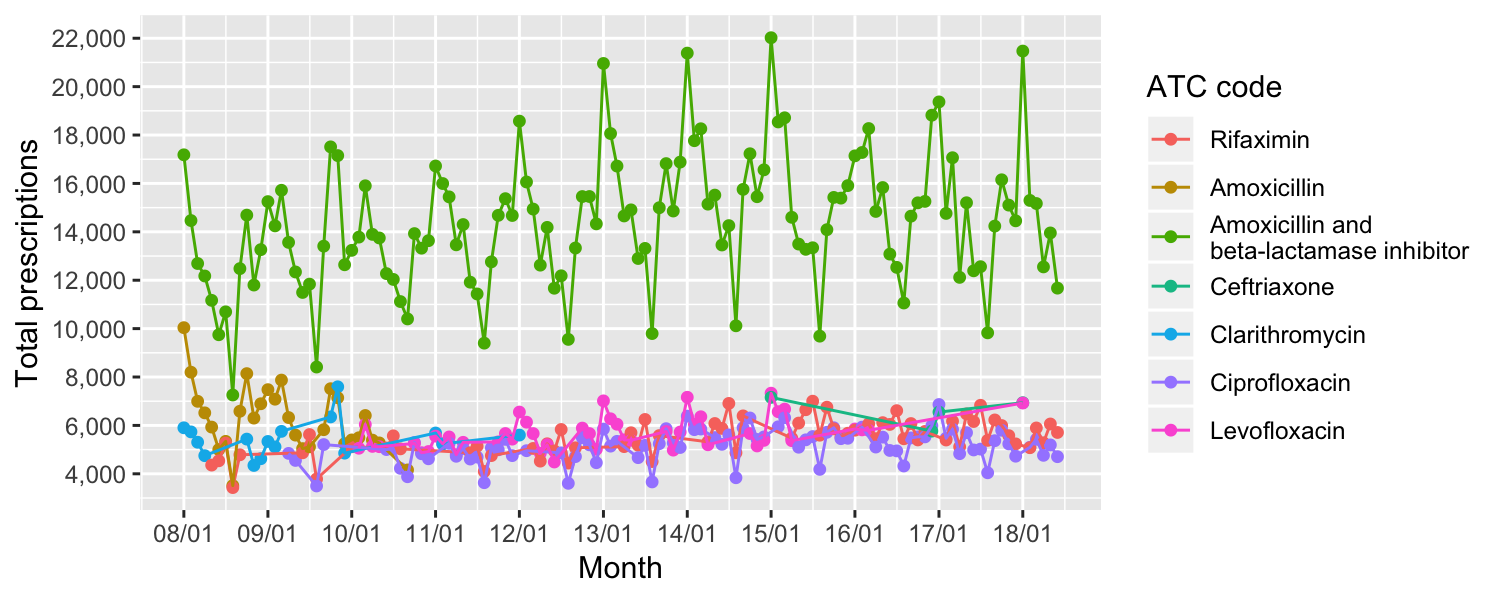
\includegraphics[scale=0.3]{../plots/top_atc-month.png}
\end{figure}

Most ATCs follow a similar pattern: the amount decreases in 2010-2012 to then have a small peak in 2016 and get lower again in 2017, similarly to the global amount of prescriptions.

The most noticeable unusual trend corresponds to amoxicillin and beta-lactose inhibitors (ATC J01CR02), which considerably detaches from the others. Amoxicillin is one of the most popular group of drugs, confirmed by global analytics on the database and USA trends\cite{usa}.

It is evident that the monthly prescriptions follow a seasonal trend: the number of prescription rises during the winter and falls during the summer.

\subsection{Comparison with ICD-9}
Since ICD-9 have some unusual trends, comparing them with antibiotics might provide additional information. The interested area comprehends ICD-9 class A, diseases of the digestive tract whose diagnoses have doubled in the span of 10 years. Antibiotics to treat this subset are:
\begin{itemize}
	\item Nyastatin;
	\item Rifaximin;
	\item Paromomycin.
\end{itemize}

Cross-checking related codes with the antibiotics dataset, rifaximin is indeed one of the most prescribed drugs, while its numbers are still considerably inferior to amoxicillin (the most popular antibiotic). Seasonality is still present, yet less pronounced. 

\begin{figure}[h]
	\centering
	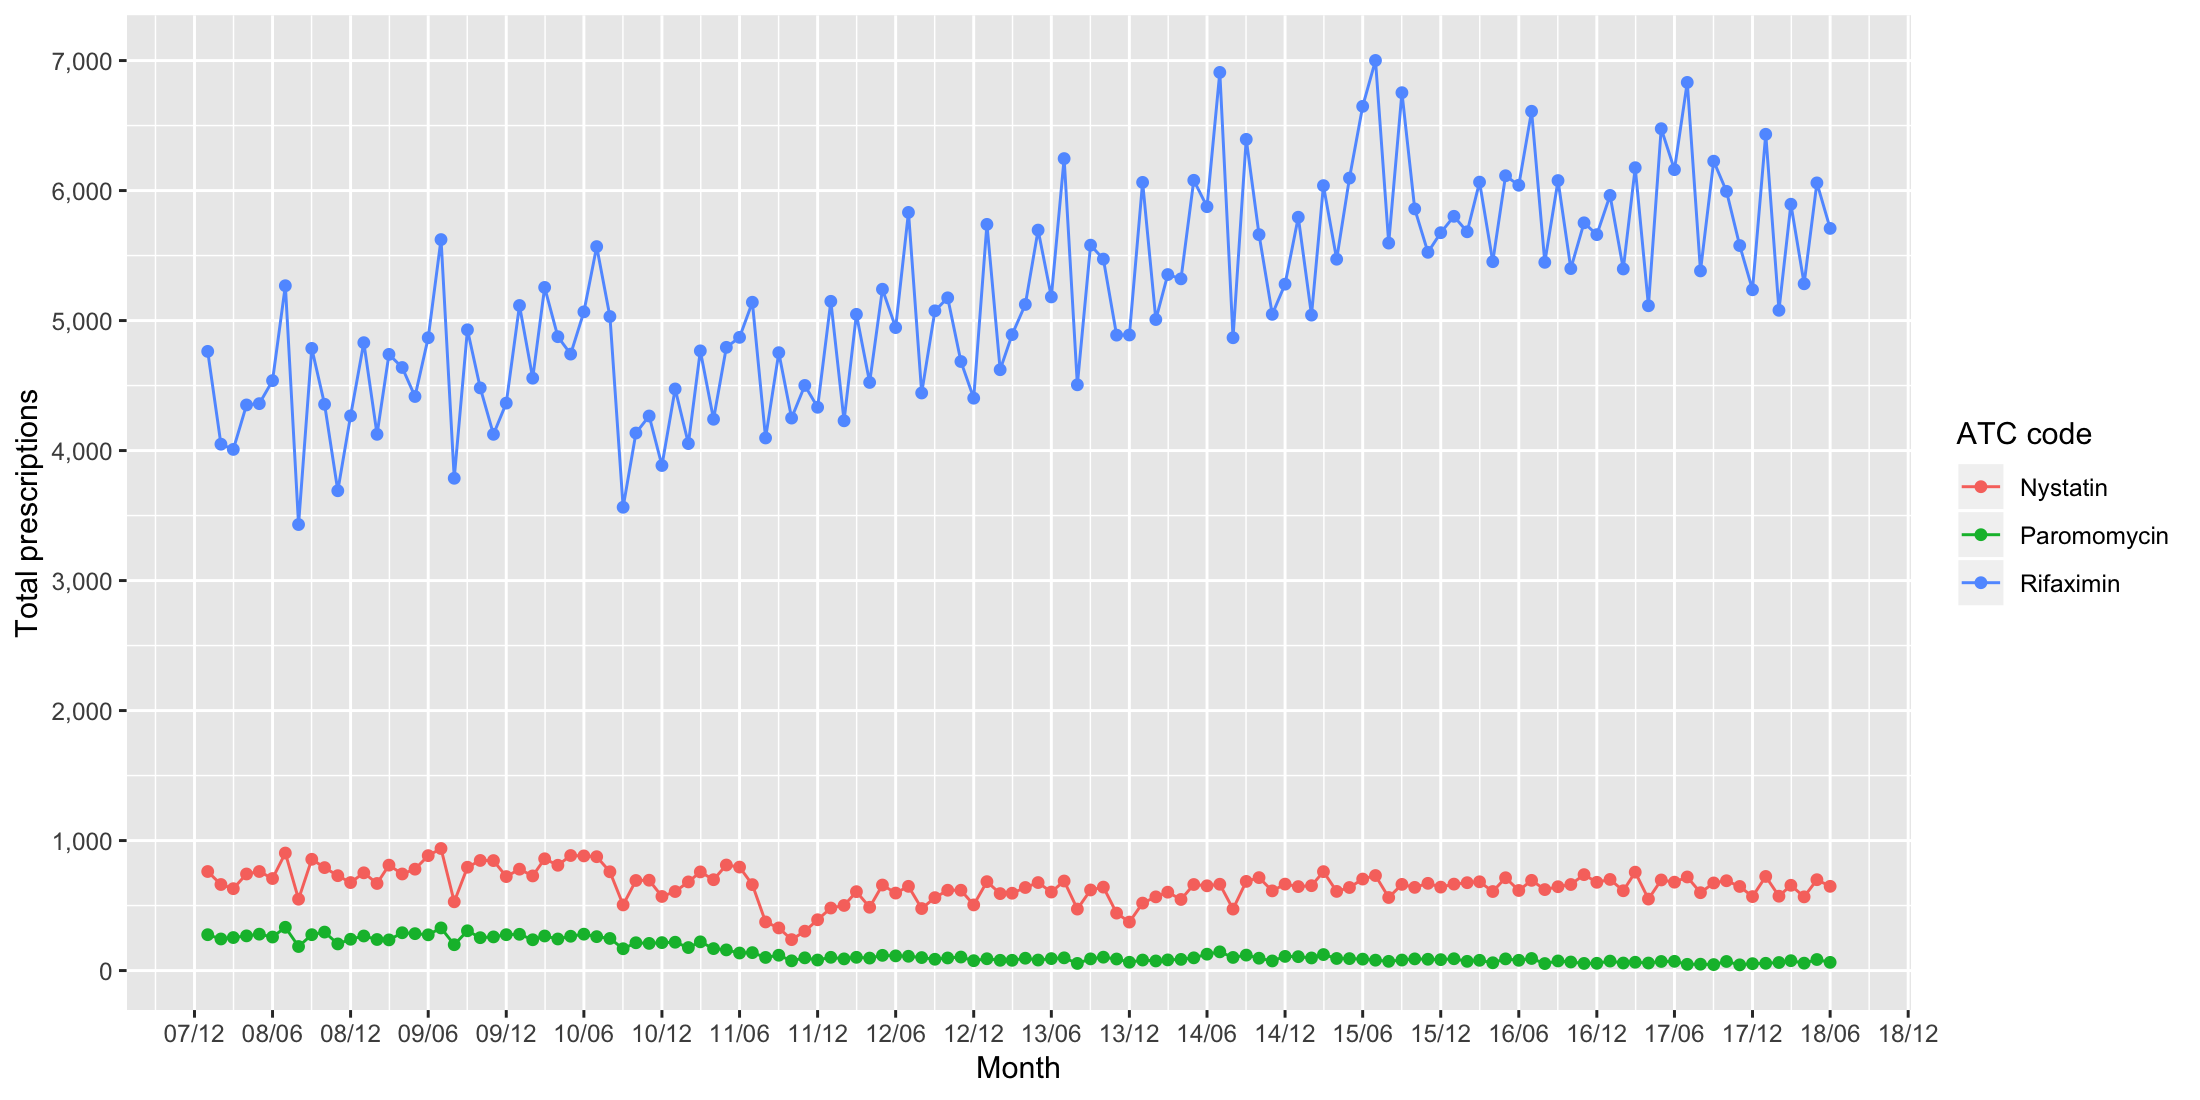
\includegraphics[scale=0.3]{../plots/top_atc_a-month.png}
\end{figure}

\section{AIC rankings}
Prescriptions with AICs don't have a public lookup table, yet drugs can be singularly searched on a public database by AIFA. Analytics have been made on the antibiotics subset of data, using the 5 most prescribed medicines for months and years.

Augmentin is the top ranked prescription, detaching from the others and with a progressive increase starting from 2010: values go up to 100 000 prescriptions in 2017, and January 2017 is the month with the maximum number.

Having a difference of 30 000 between 2010 and 2017 without a correspondent increase of diagnoses shows frequent episodes of antibiotic resistance and overprescribing.

\begin{figure}[h]
	\centering
	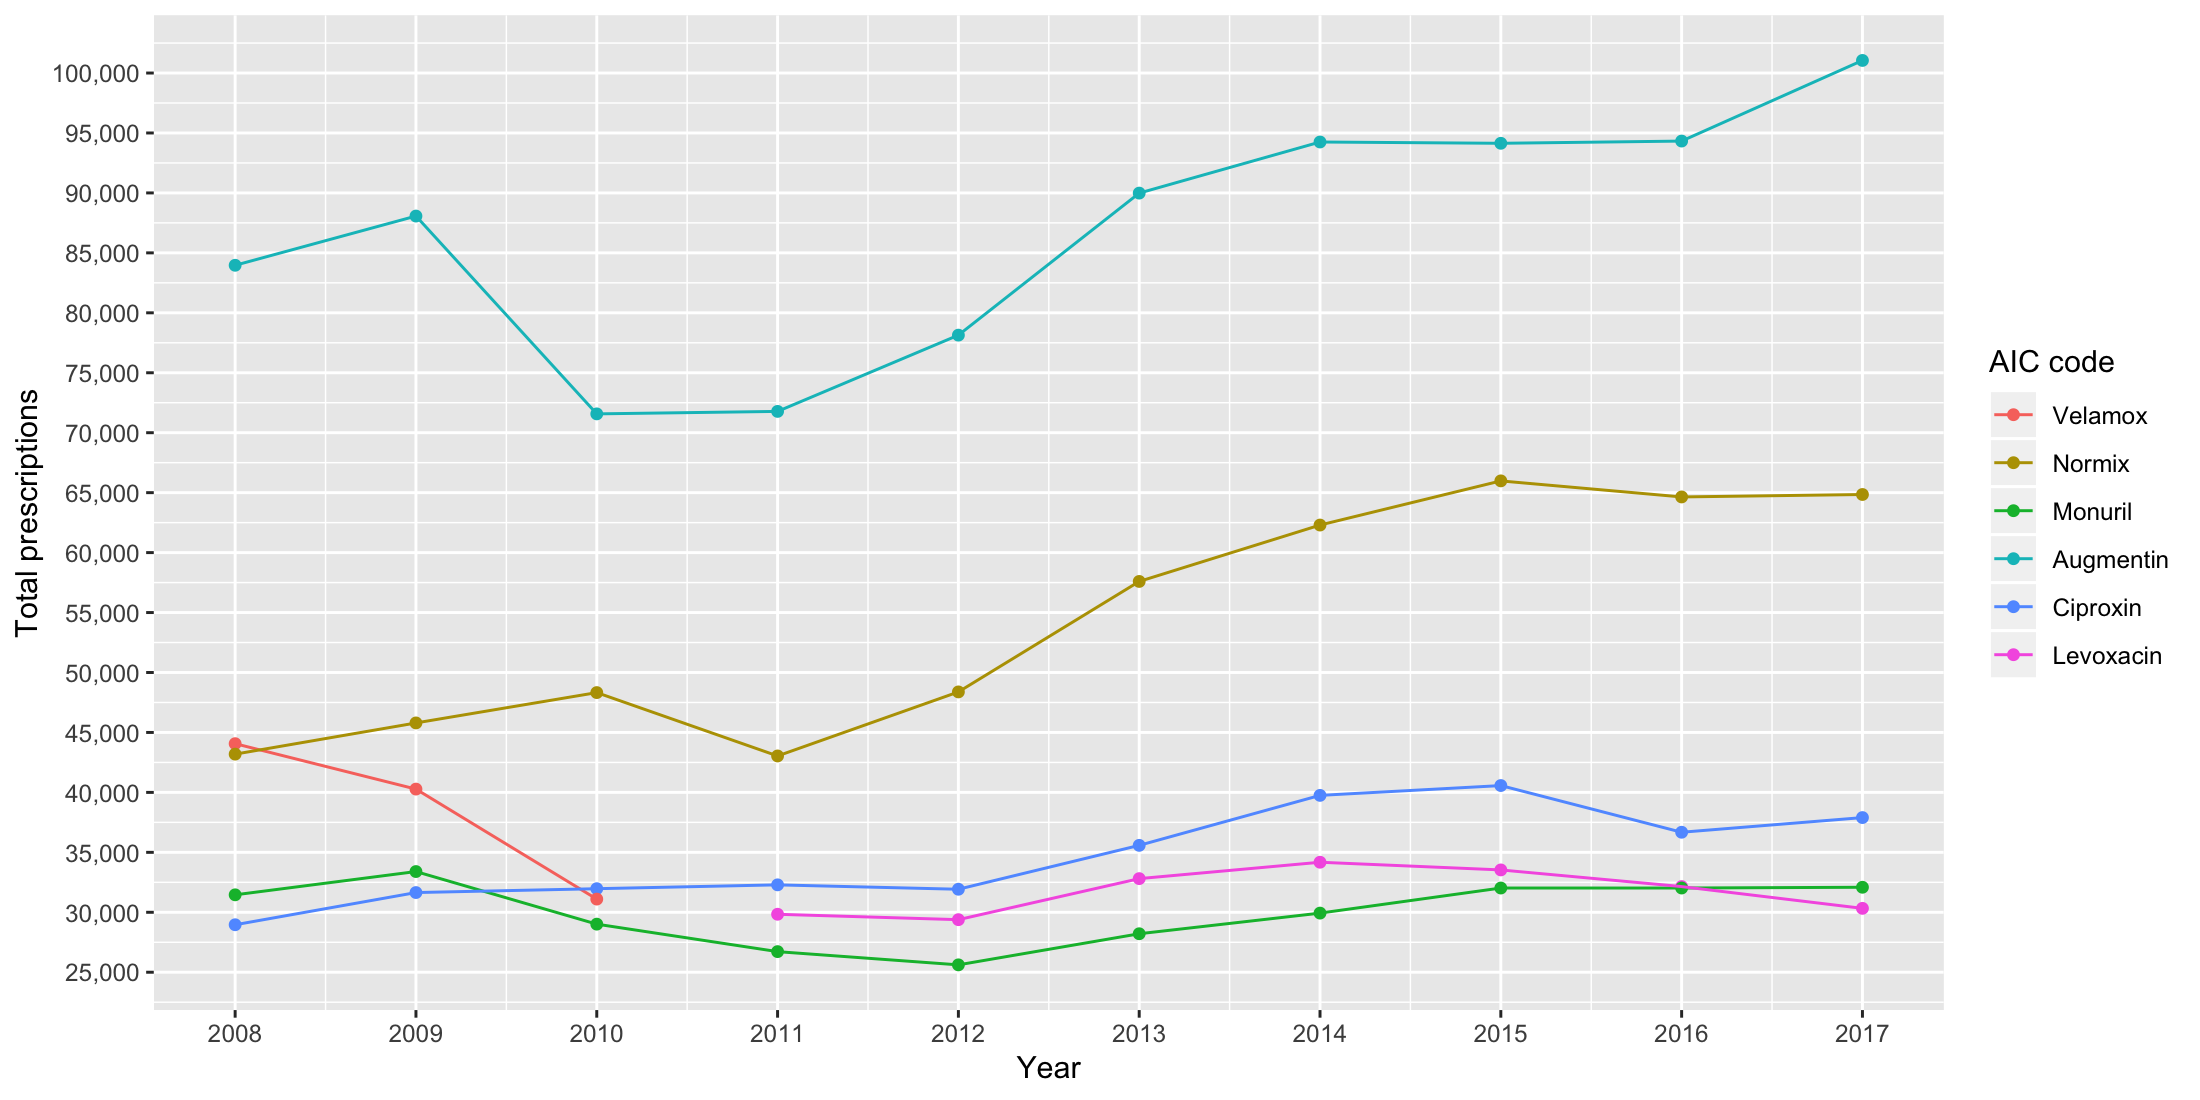
\includegraphics[scale=0.3]{../plots/top_aic-year.png}
\end{figure}

\begin{figure}[h]
	\centering
	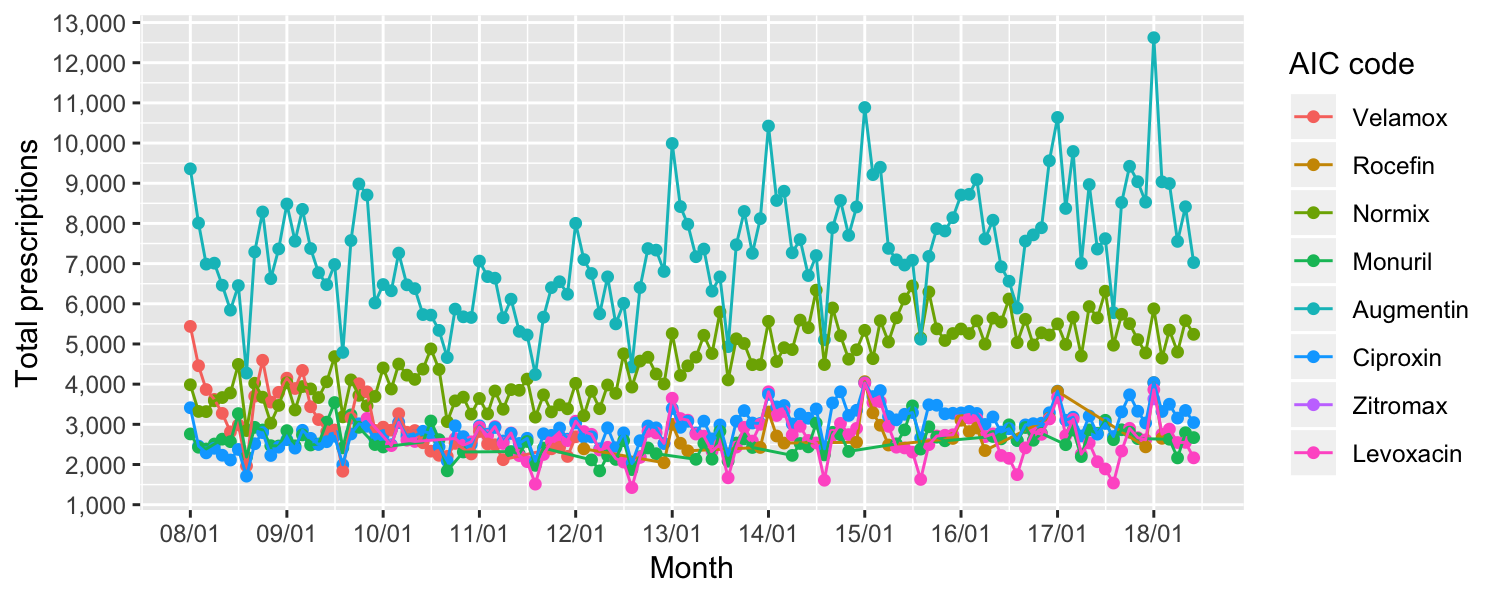
\includegraphics[scale=0.3]{../plots/top_aic-month.png}
\end{figure}

The drug Velamox has an opposite behaviour compared to the others: while most medicines are increasing their number of prescriptions, while Velamox is subject to progressive decrease until disappearance from the most prescribed drugs.

A better understanding between orders of magnitudes could be obtained counting the total prescriptions in 10 years of the most common AICs:

\begin{center}
	\begin{tabular}{c|c|c}
		Code & Prescriptions & Antibiotic \\
		\hline
		026089019 & 934 942 & Augmentin 875 mg + 125 mg 12 coated tablets \\
		\hline
		025300029 & 586 782 & Normix 200 mg 12 coated tablets\\
		\hline
		026664021 & 373 720 & Ciproxin 500 mg 6 coated tablets \\
		\hline
		033940038 & 264 604 & Levoxacin 500 mg 5 coated tablets \\
		\hline
		025680024 & 229 816 & Monuril 3 g 2 sachets \\
		\hline
		023097102 & 132 787 & Velamox 1 g 12 dispersible tablets \\
	\end{tabular}
\end{center}

\subsection{An insight on Velamox}
Velamox, according to AIFA, is an amoxicillin-based drug used for respiratory trait, ear and genital infections. It is sold in different packages, whose the most popular is the 1 g dispersible tablets with 12 tablets.

Since the general trending of most prescribed antibiotics only gave a partial vision of the comparisons between products, a complete chart is extracted using Velamox and three other popular drugs: Augmentin, Normix and Levoxacin. The difference is evident:

\begin{figure}[h]
	\centering
	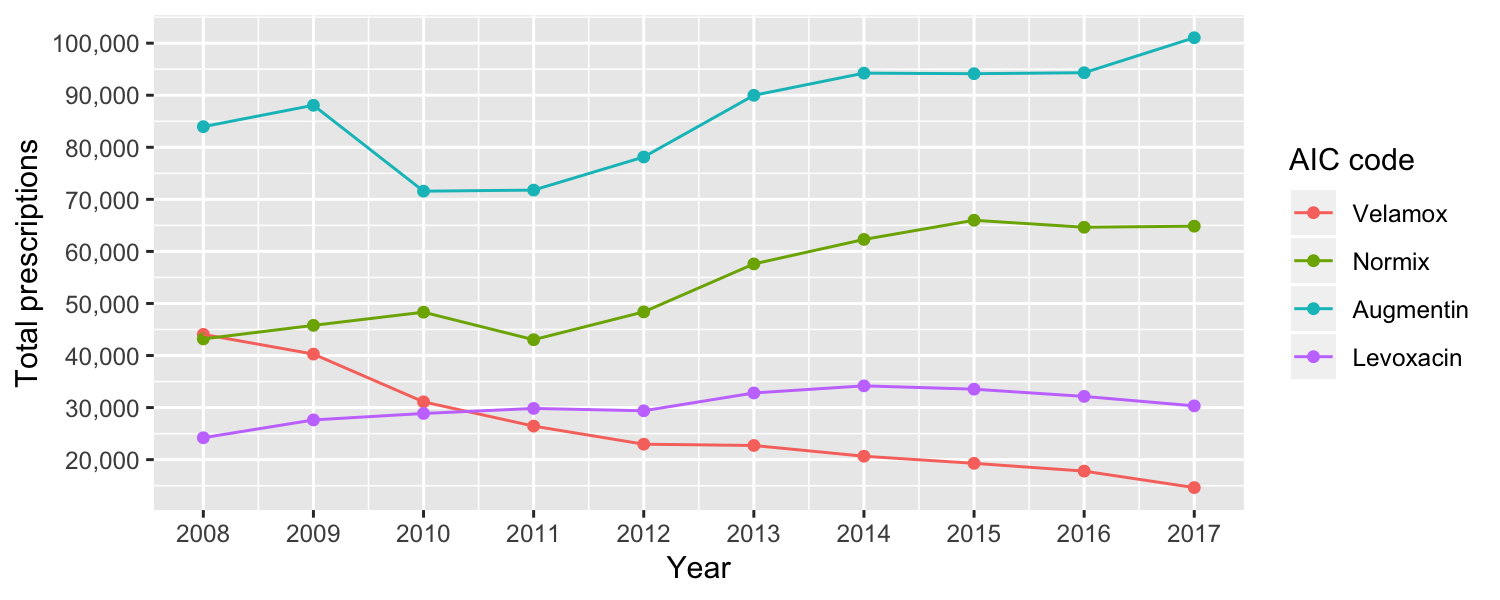
\includegraphics[scale=0.3]{../plots/aic_4-year.png}
\end{figure}

The first hypothesis of such a drastic drop of a product is its switch with another one, changing prescriptive habits of doctors. If that was the case, graphs related to the specific subset of patients would have a correspondent rise of values belonging to another antibiotic.

Velamox in 2008, the year of maximum amount of prescriptions, has been given to approximately 32 000 patients. Extracting only the top 3 antibiotic prescriptions of those, in the last 10 years, along with Velamox, shows no substitution by another drug.

The fall starts in 2009, having a drop of 30 000 units, and gradually continues until 2017 with only 3 037 prescriptions:

\begin{figure}[h]
	\centering
	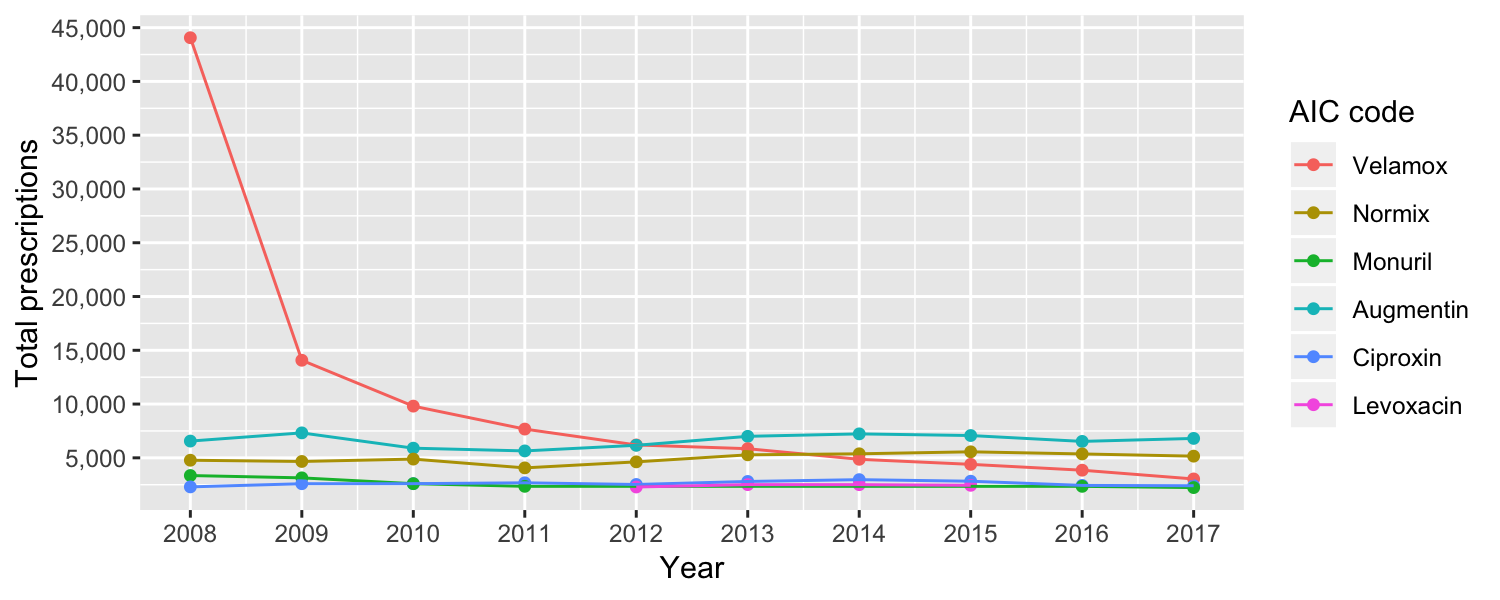
\includegraphics[scale=0.3]{../plots/top_aic_subset-year.png}
\end{figure}

ATC trends related to Velamox's AIC show usual patterns: since the same ATC is linked with more products, the curve is still leaning upwards, yet there is an offset equal to the decrease in Velamox.

Since analysis on a subset of patients gives little insight, a wider time range can give additional information on a complete picture of global trends. 

Further knowledge is obtained counting the total number of Velamox prescriptions among all patients from 2000 to 2017:

\begin{figure}[h]
	\centering
	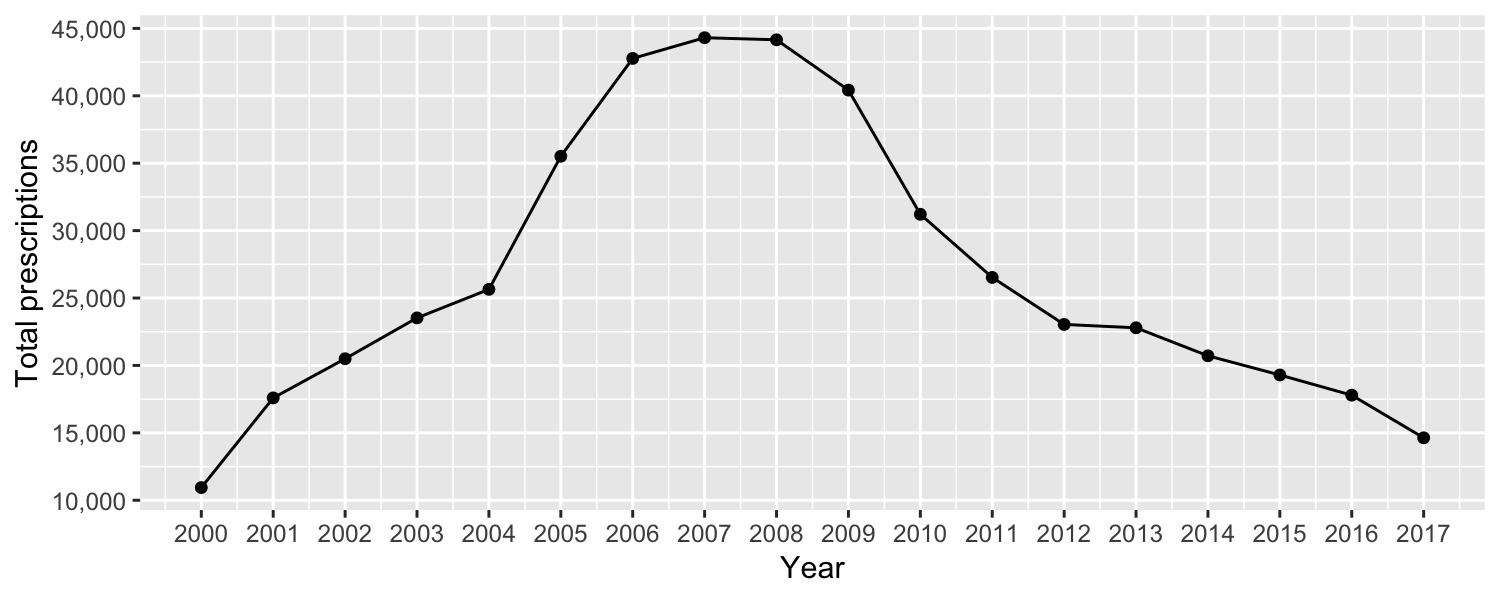
\includegraphics[scale=0.3]{../plots/velamox-year.png}
\end{figure}

Velamox has acquired popularity from 2005 to 2010, when antibiotic resistance still hadn't been recognised as a problem and before the advent of generic drugs, yet this does not provide an explanation for the decrease.

Additional analysis is made on the subset of 32 000 patients:
\begin{itemize}
	\item 1 500 are dead;
	\item 8 000 have changed GP;
	\item 18 000 are females;
	\item 14 000 are males;
	\item 16 000 are born before 1960.
\end{itemize}

General practitioners assigned to the subset of patients have generally decreased their prescriptions quota, roughly halving it comparing 2008 to 2017.

AIFA has also revoked authorisation for most instances of Velamox packages, only leaving three out of ten. The company which produces the drug, Mediolanum Farmacy, has been acquired by Neopharmed Gentili in 2018.

Summarising, changes in Velamox prescriptions are partially caused by:
\begin{itemize}
	\item Doctors gradually abandoning it after authorisation revoking;
	\item Patients dying or switching doctor;
	\item Substitutions with other drugs, none of whose is prescribed enough to have a significant trend, such as generics;
	\item Different advertisement campaigns after the company acquisition.
\end{itemize}

\subsection{An insight on Augmentin}
After analysing a drug with an unusual decrease, the focus can shift to the opposite side, considering the one with a noticeable increase.

Augmentin is the most prescribed antibiotic, with an almost constant positive trend:

\begin{figure}[h]
	\centering
	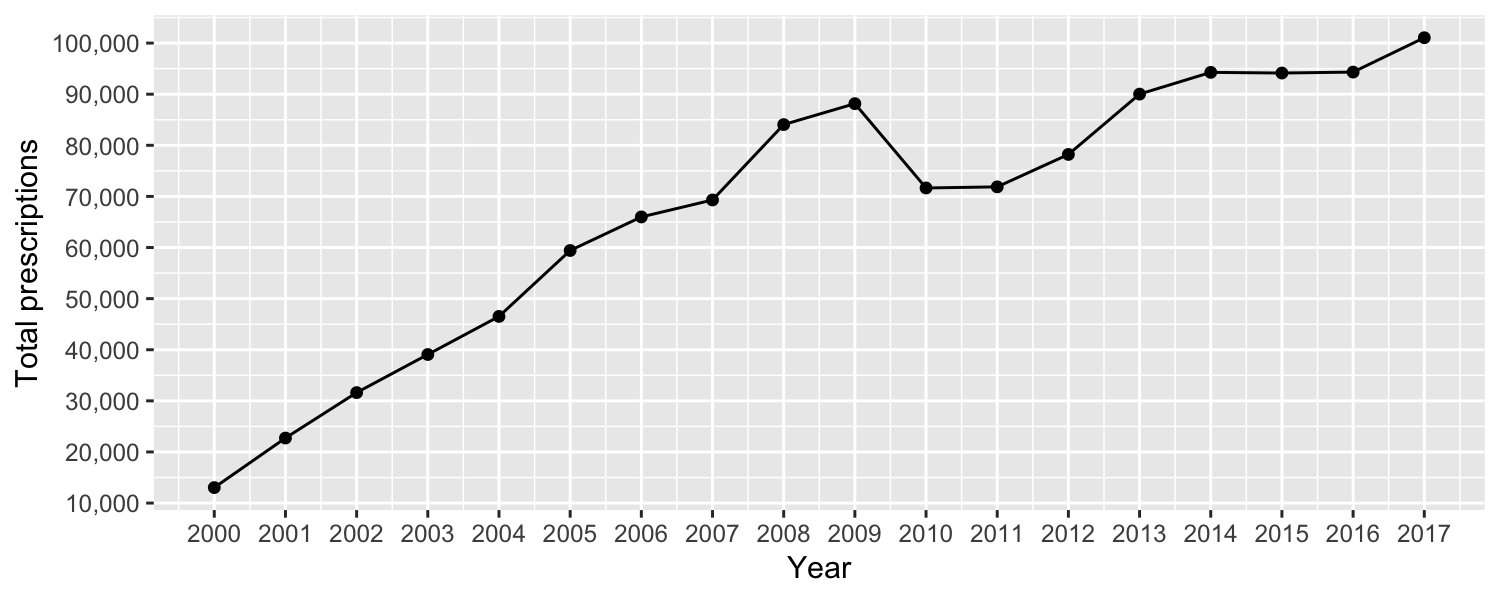
\includegraphics[scale=0.3]{../plots/augmentin-year.png}
\end{figure}

2010 and 2011 have lower values, possibly explained by the Italian economic crisis or the diffusion of generic drugs. Starting from 2013 numbers continue to rise, reaching their highest peak in 2017.

Most Augmentin consumers are adults in the range of 45-64 years of age, following global trends previously obtained.

\begin{figure}[h]
	\centering
	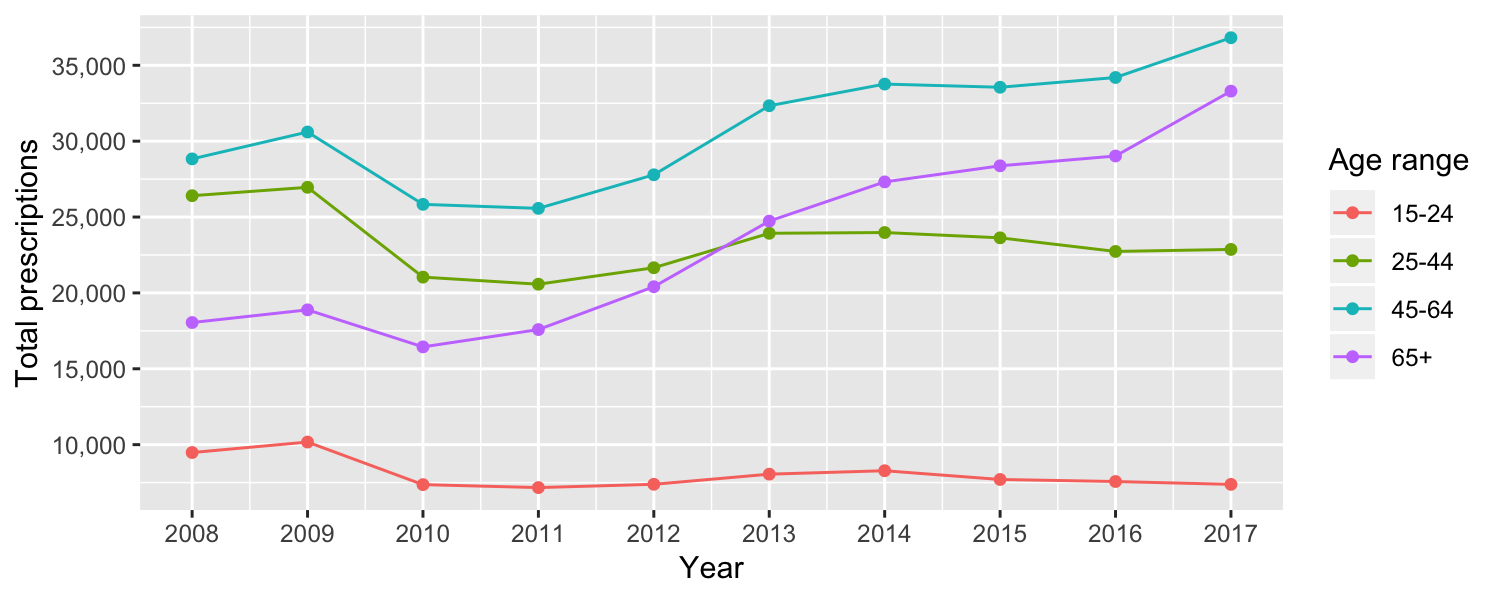
\includegraphics[scale=0.3]{../plots/augmentin_age-year.png}
\end{figure}

\subsection{According to geographical area}
There is information loss on geographical area of patients, therefore it is necessary to extract a further subset of antibiotic prescriptions, applying a level of cleansing.

Patients with complete and correct province of residence fields are selected, obtaining:
\begin{itemize}
	\item 590 472 patients, 74,34\%;
	\item 7 458 312 prescriptions, 88,94\%.
\end{itemize}

Campania has five provinces: Naples, Avellino, Caserta, Benevento and Salerno. Analytics are expected to show an uniform distribution of prescriptions among those, yet outcomes are skewed towards Naples (significantly bigger) and other cities.

Top 5 municipalities for total prescriptions in 2008-2017:
\begin{center}
	\begin{tabular}{c|c|c}
		Postcode & Province & Prescriptions \\
		\hline
		063049 & Naples & 2 854 056 \\
		\hline
		063002 & Afragola & 618 519 \\
		\hline
		063024 & Castellammare di Stabia & 497 309 \\
		\hline
		063005 & Arzano & 314 640 \\
		\hline
		063035 & Gragnano & 210.960 \\
	\end{tabular}
\end{center}

Prescriptions come from 932 different cities, while there are 550 distinct cities in Campania. This implies a slice of patients having residence in a different place outside the region.

Results might be altered by the non-uniform provenance of doctors and patients (mostly from the Naples area), and other big municipalities have large population although not qualifying as provinces. 

Discrepancies among provinces are also shown by the following plot, identifying trends:
\begin{figure}[h]
	\centering
	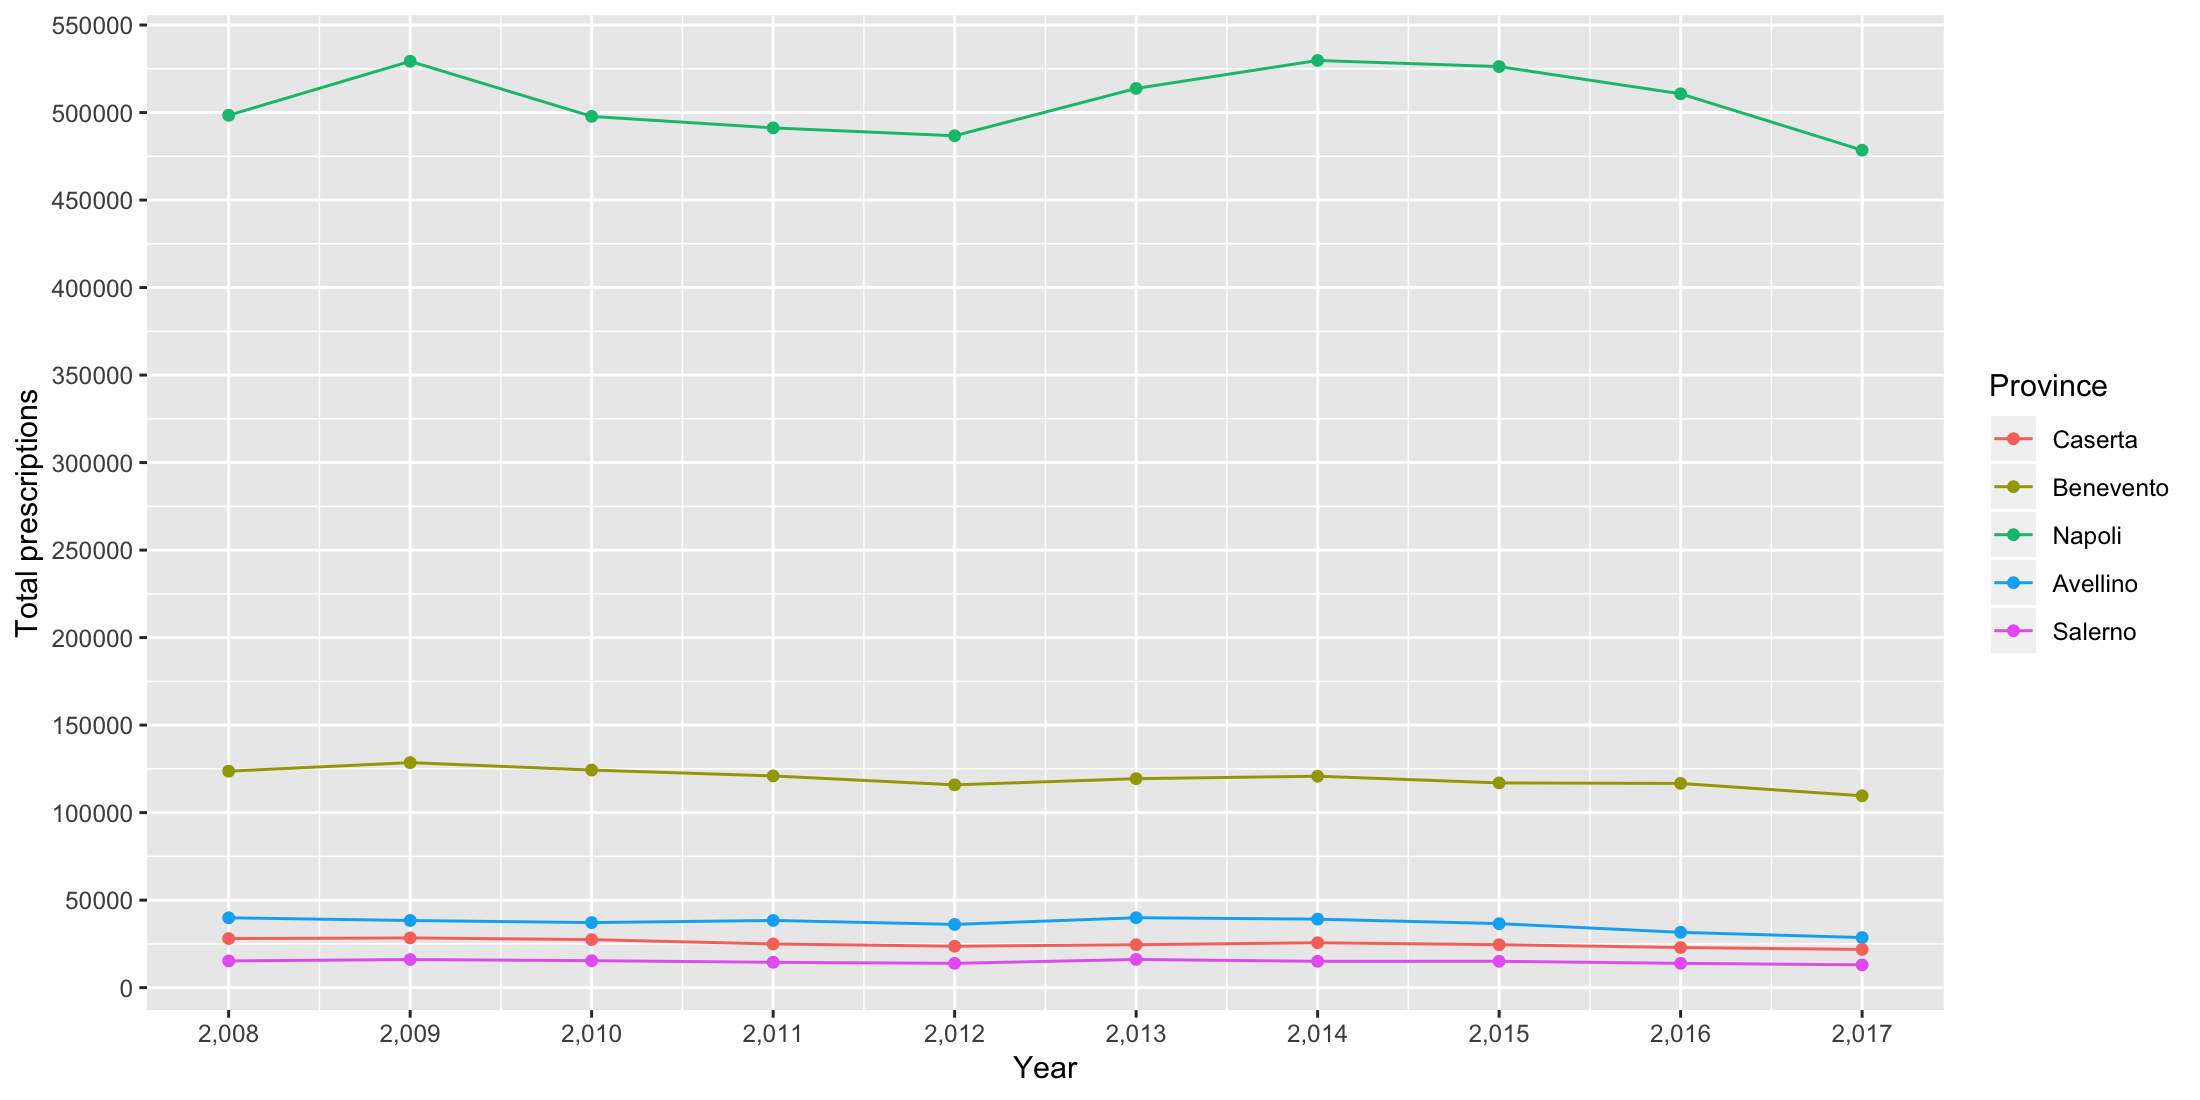
\includegraphics[scale=0.3]{../plots/provinces.png}
\end{figure}

\subsubsection{Pharmacies}
The number of pharmacies divided by province with related population (ISTAT 2018) confirms the gap between Naples and the others: 
\begin{enumerate}
	\item 857 pharmacies in the Naples area, 3 101 002 inhabitants;
	\item 375 pharmacies in the Salerno area, 1 101 763 inhabitants;
	\item 254 pharmacies in the Caserta area, 923 445 inhabitants;
	\item 161 pharmacies in the Avellino area, 421 523 inhabitants;
	\item 107 pharmacies in the Benevento area, 279 127 inhabitants.
\end{enumerate}

\section{ATC and AIC trends}

\subsection{By sex}

\subsection{By age}
Analytics by age are deployed dividing the subset in the 5 official age ranges, however since patients in the youngest group should receive prescriptions by paediatricians and there is no related information in the database, the range 1-14 has to be considered incorrect and therefore removed.

This causes a difference of approximately 150 000 tuples, and the remaining ones are arranged by age of patient counting the amount of prescriptions in 2008-2017:

\begin{center}
	\begin{tabular}{c|c|c}
		Age range & Prescriptions & Mean\\
		\hline
		15-24 & 643 540 & 5,25 \\
		\hline
		25-44 & 1 776 228 & 7,29 \\
		\hline
		45-64 & 2 674 494 & 10,81 \\
		\hline
		65+ & 3 115 334 & 16,16 \\
	\end{tabular}
\end{center}

A patient on average receives 9,8 prescriptions in 10 years, but there are big differences between older and younger people: the number progressively increases.

ATC and AIC popular codes are related, observing that some of the most common ones gets prescribed starting from an early age while others are prevalent between higher ranges.

5 top AICs and ATCs for age, yearly and monthly: % todo fixare i grafici, togliere qualche etichetta

\begin{figure}[h]
	\centering
	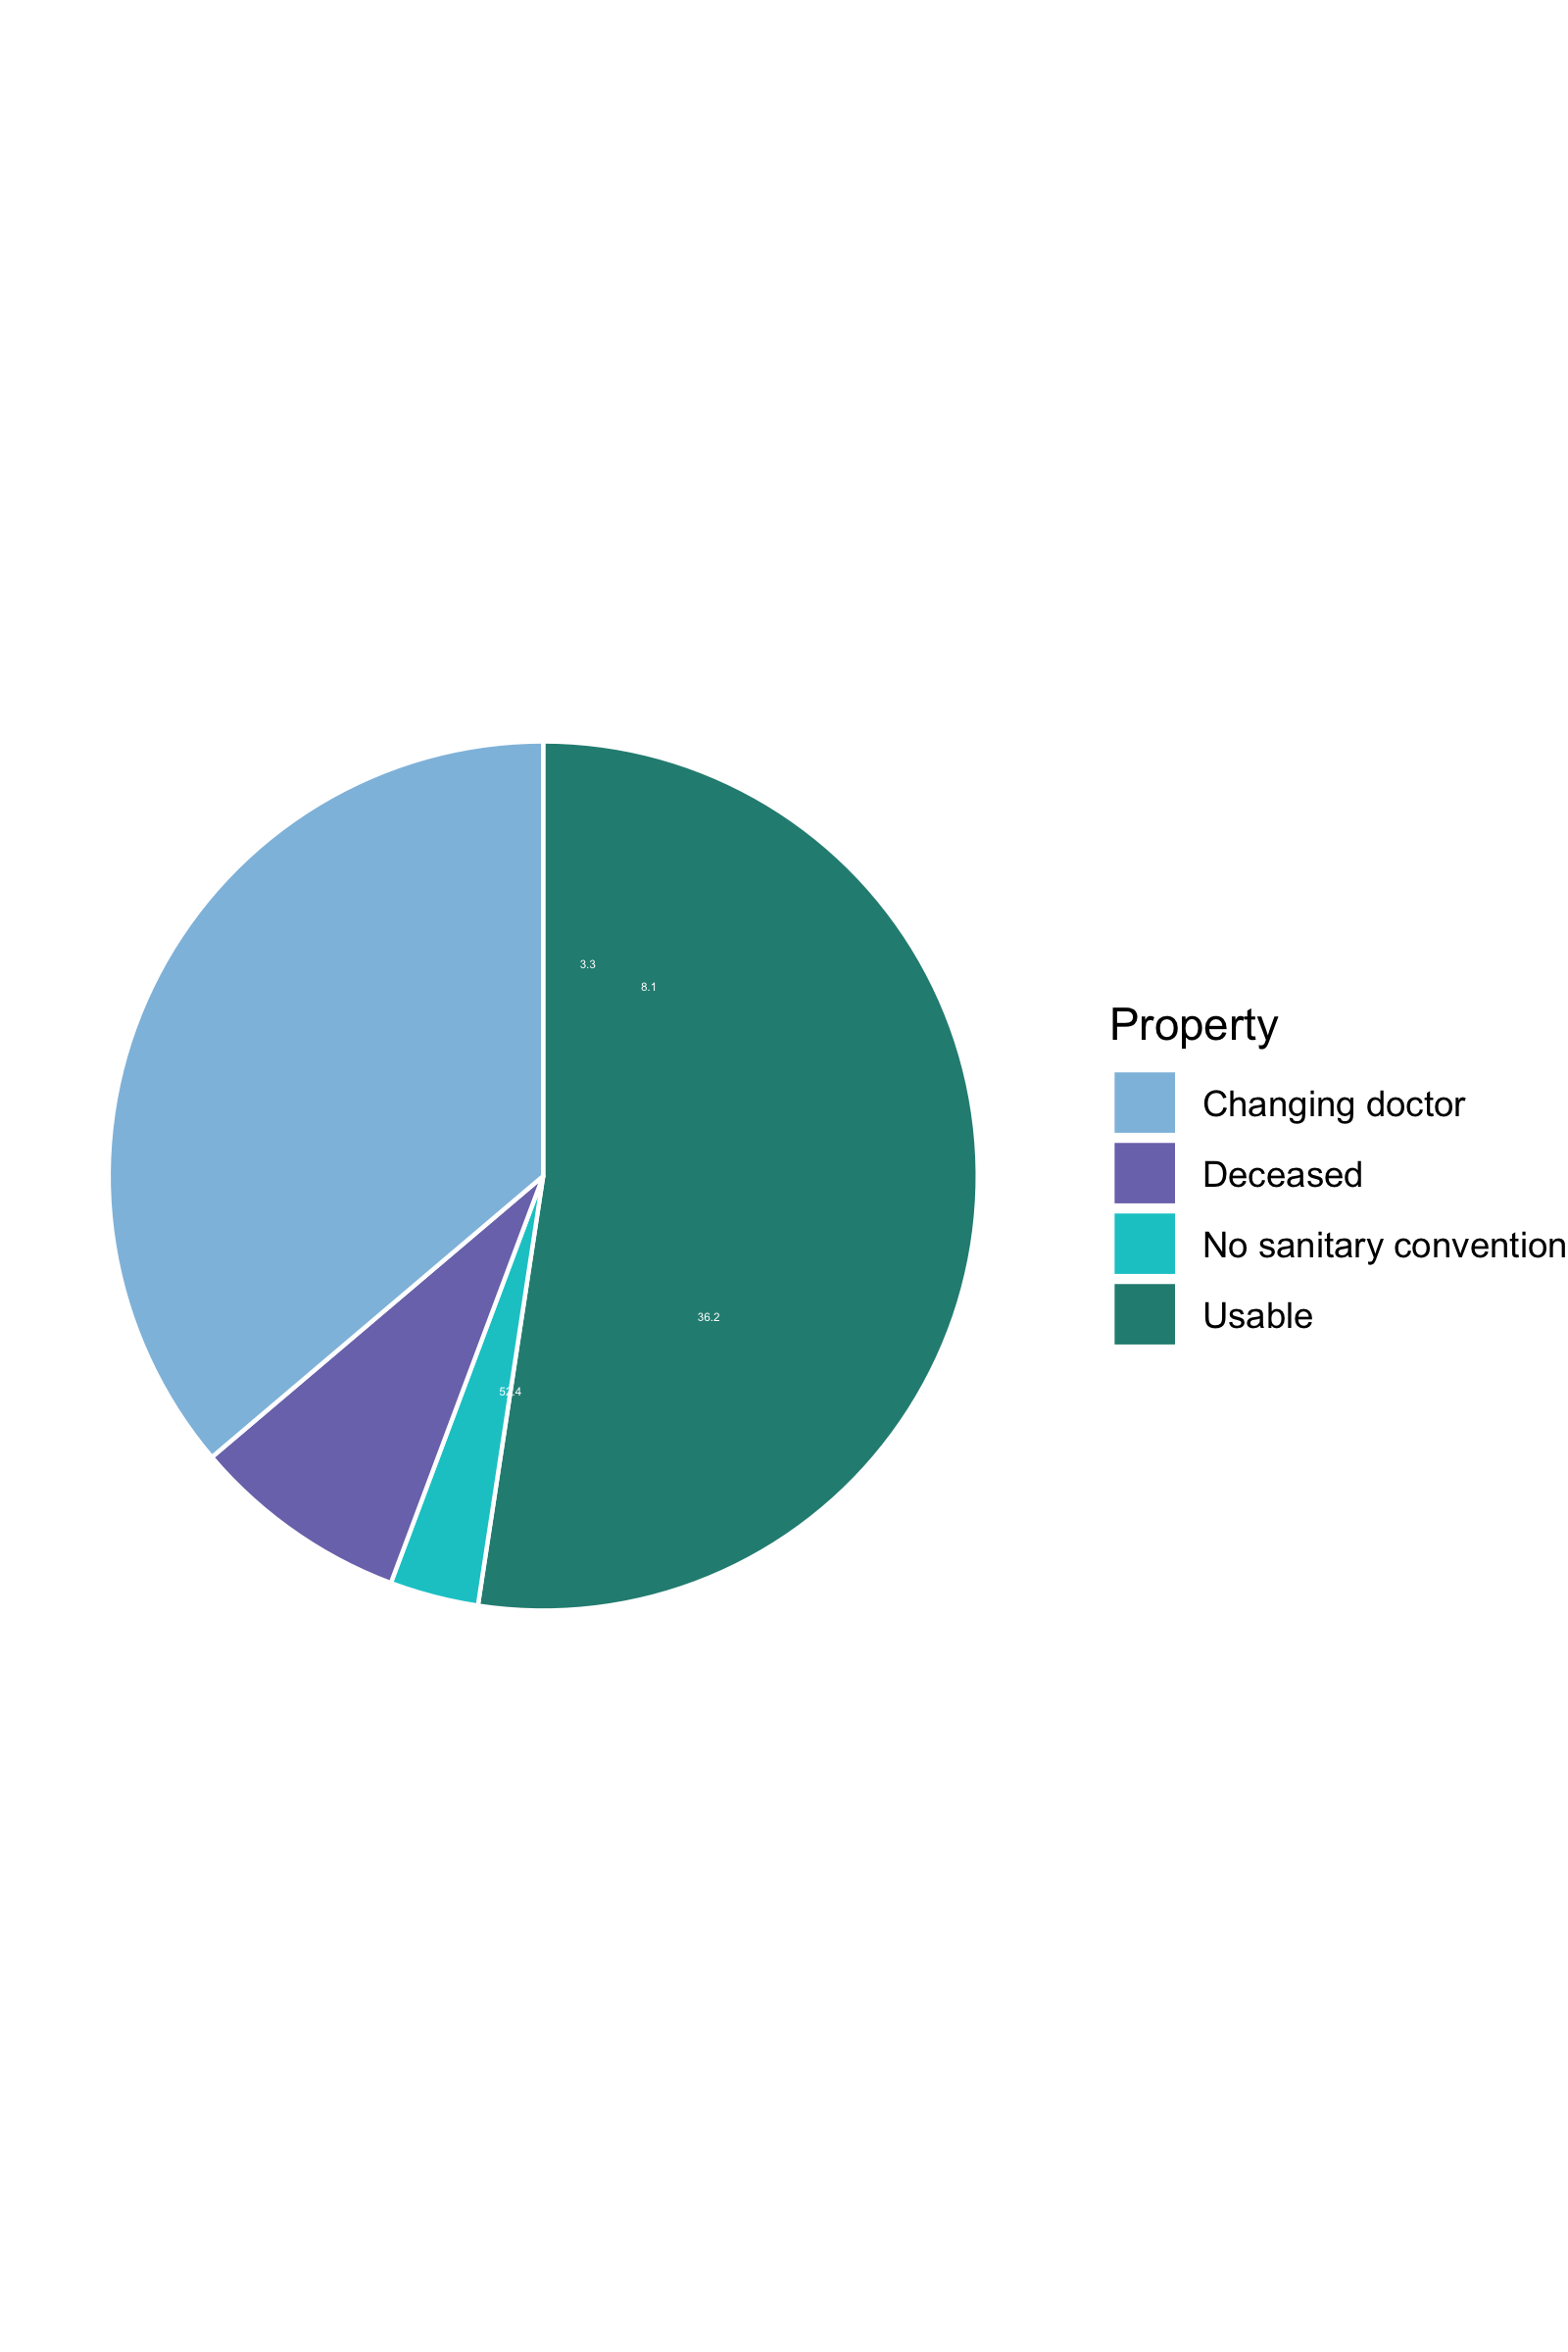
\includegraphics[scale=0.29]{../plots/top_atc_age-year.png}
\end{figure}

\begin{figure}[h]
	\centering
	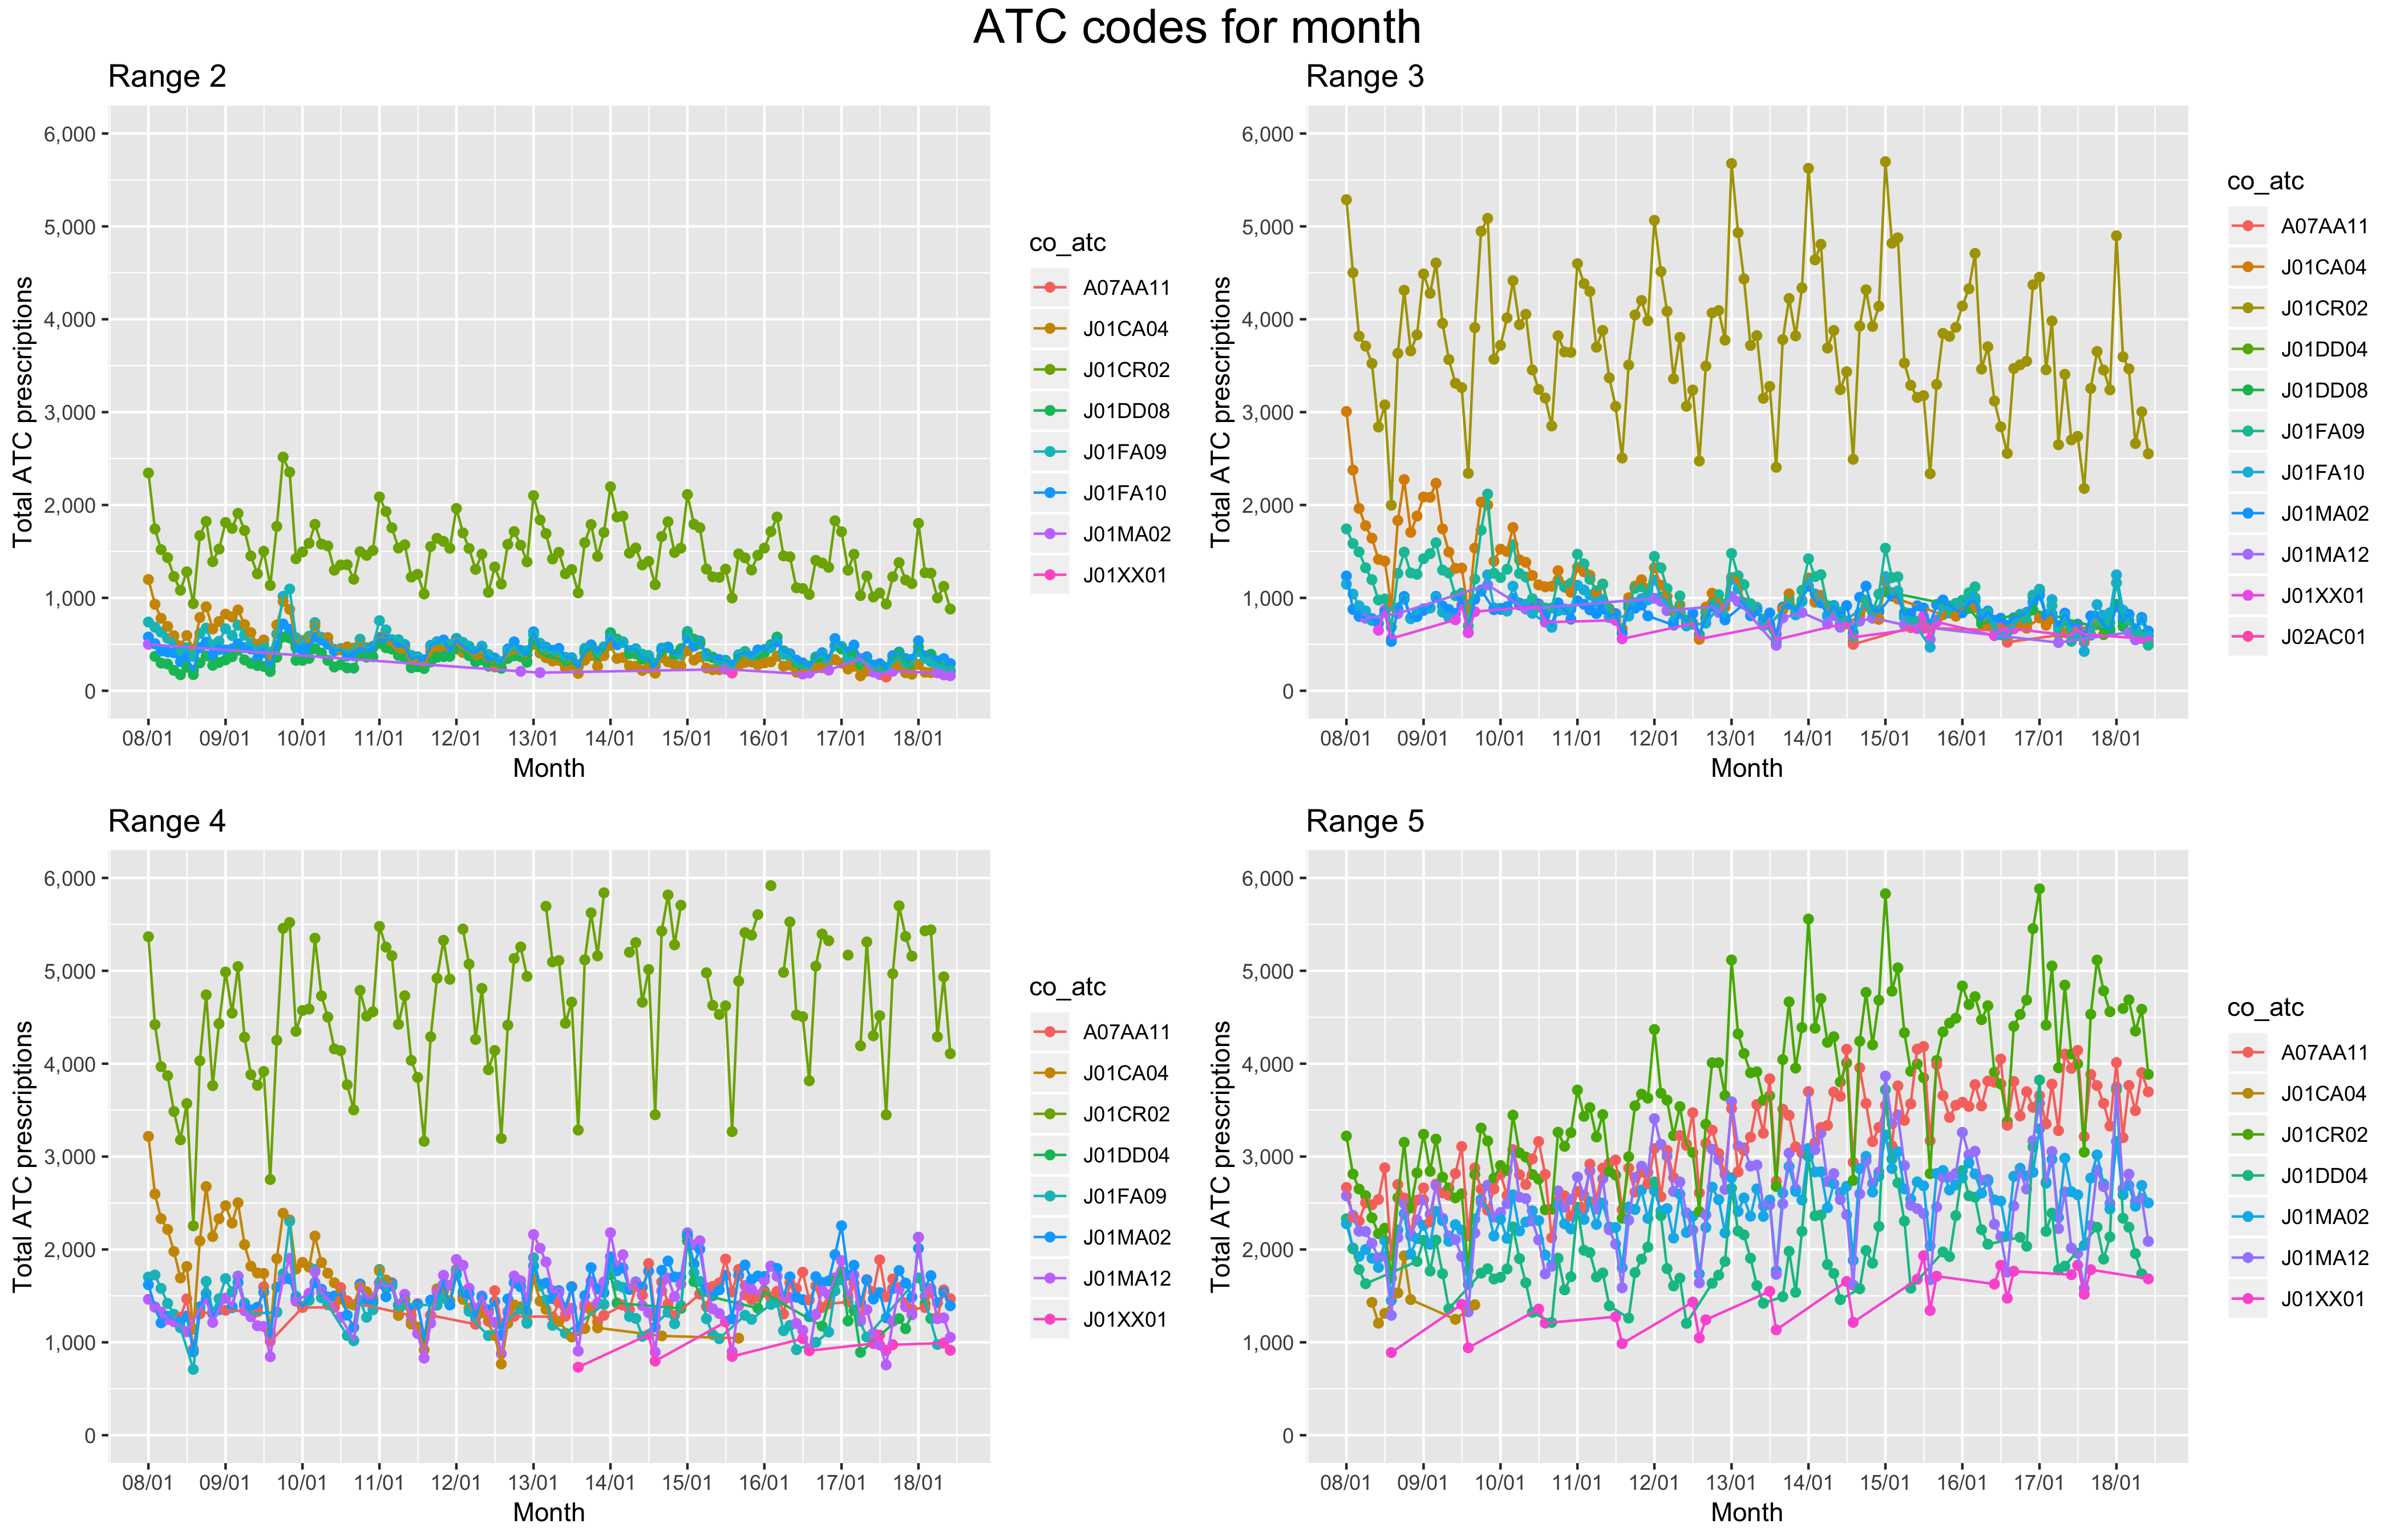
\includegraphics[scale=0.29]{../plots/top_atc_age-month.png}
\end{figure}

\begin{figure}[h]
	\centering
	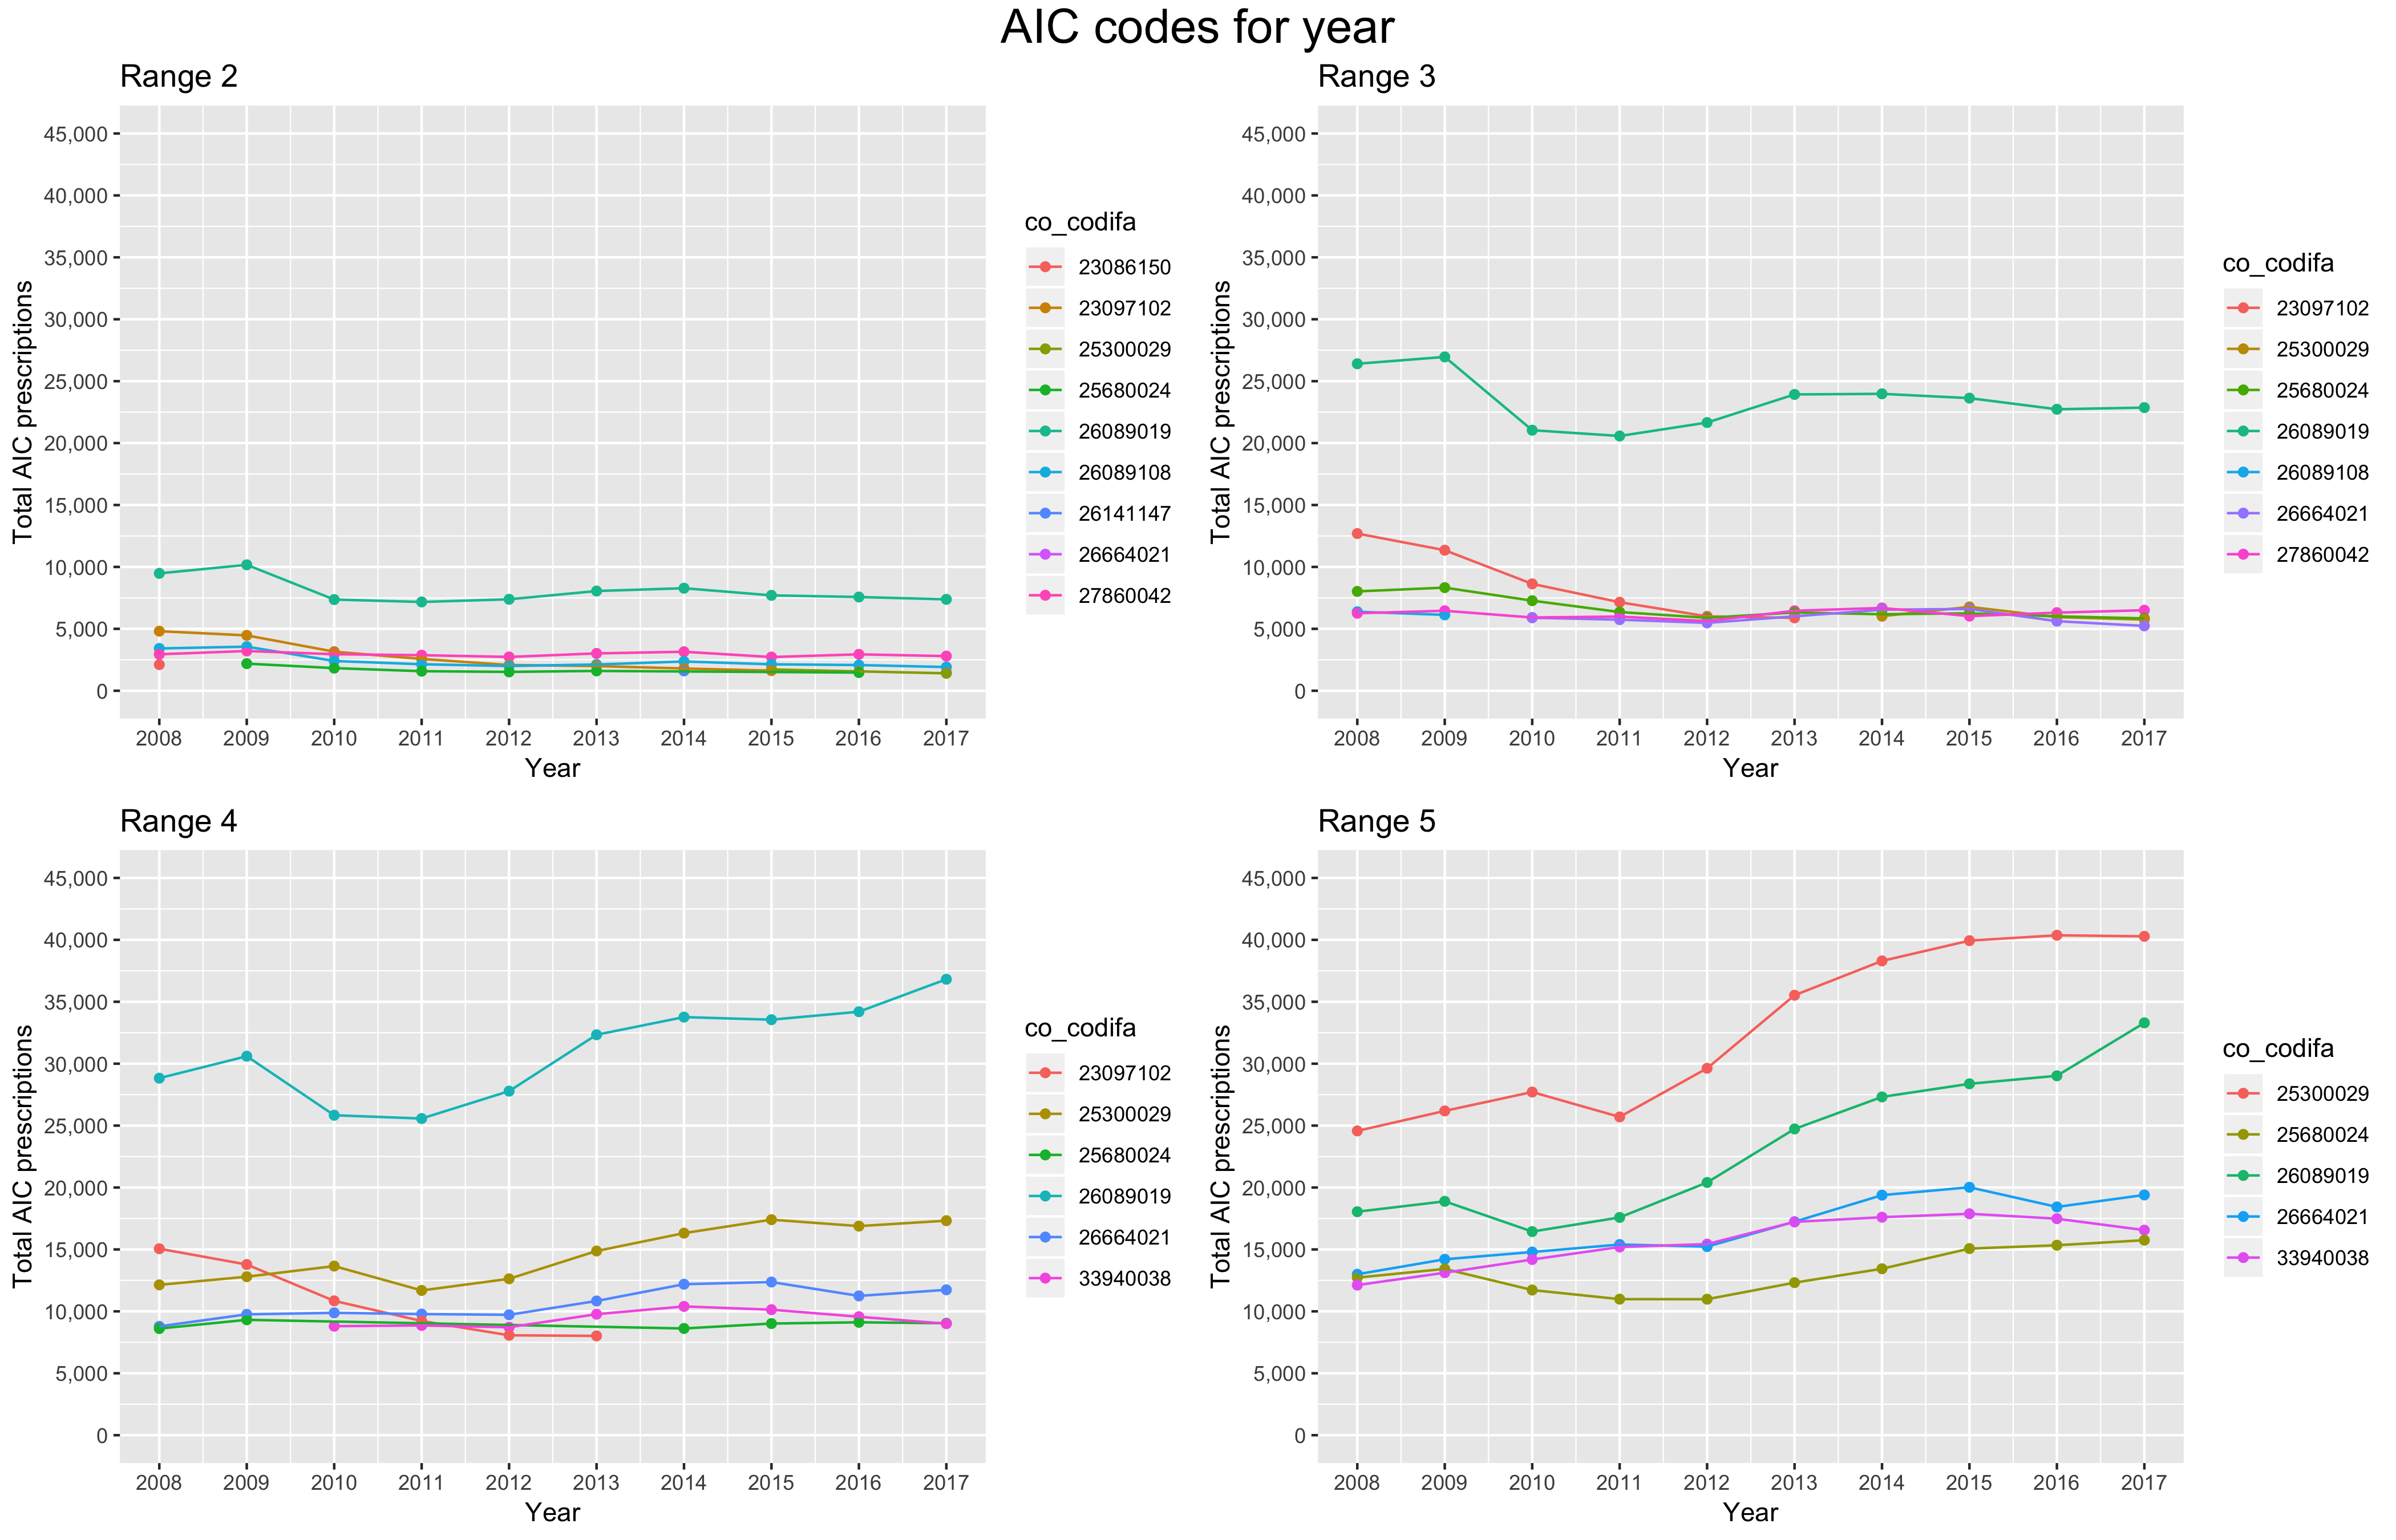
\includegraphics[scale=0.29]{../plots/top_aic_age-year.png}
\end{figure}

\begin{figure}[h]
	\centering
	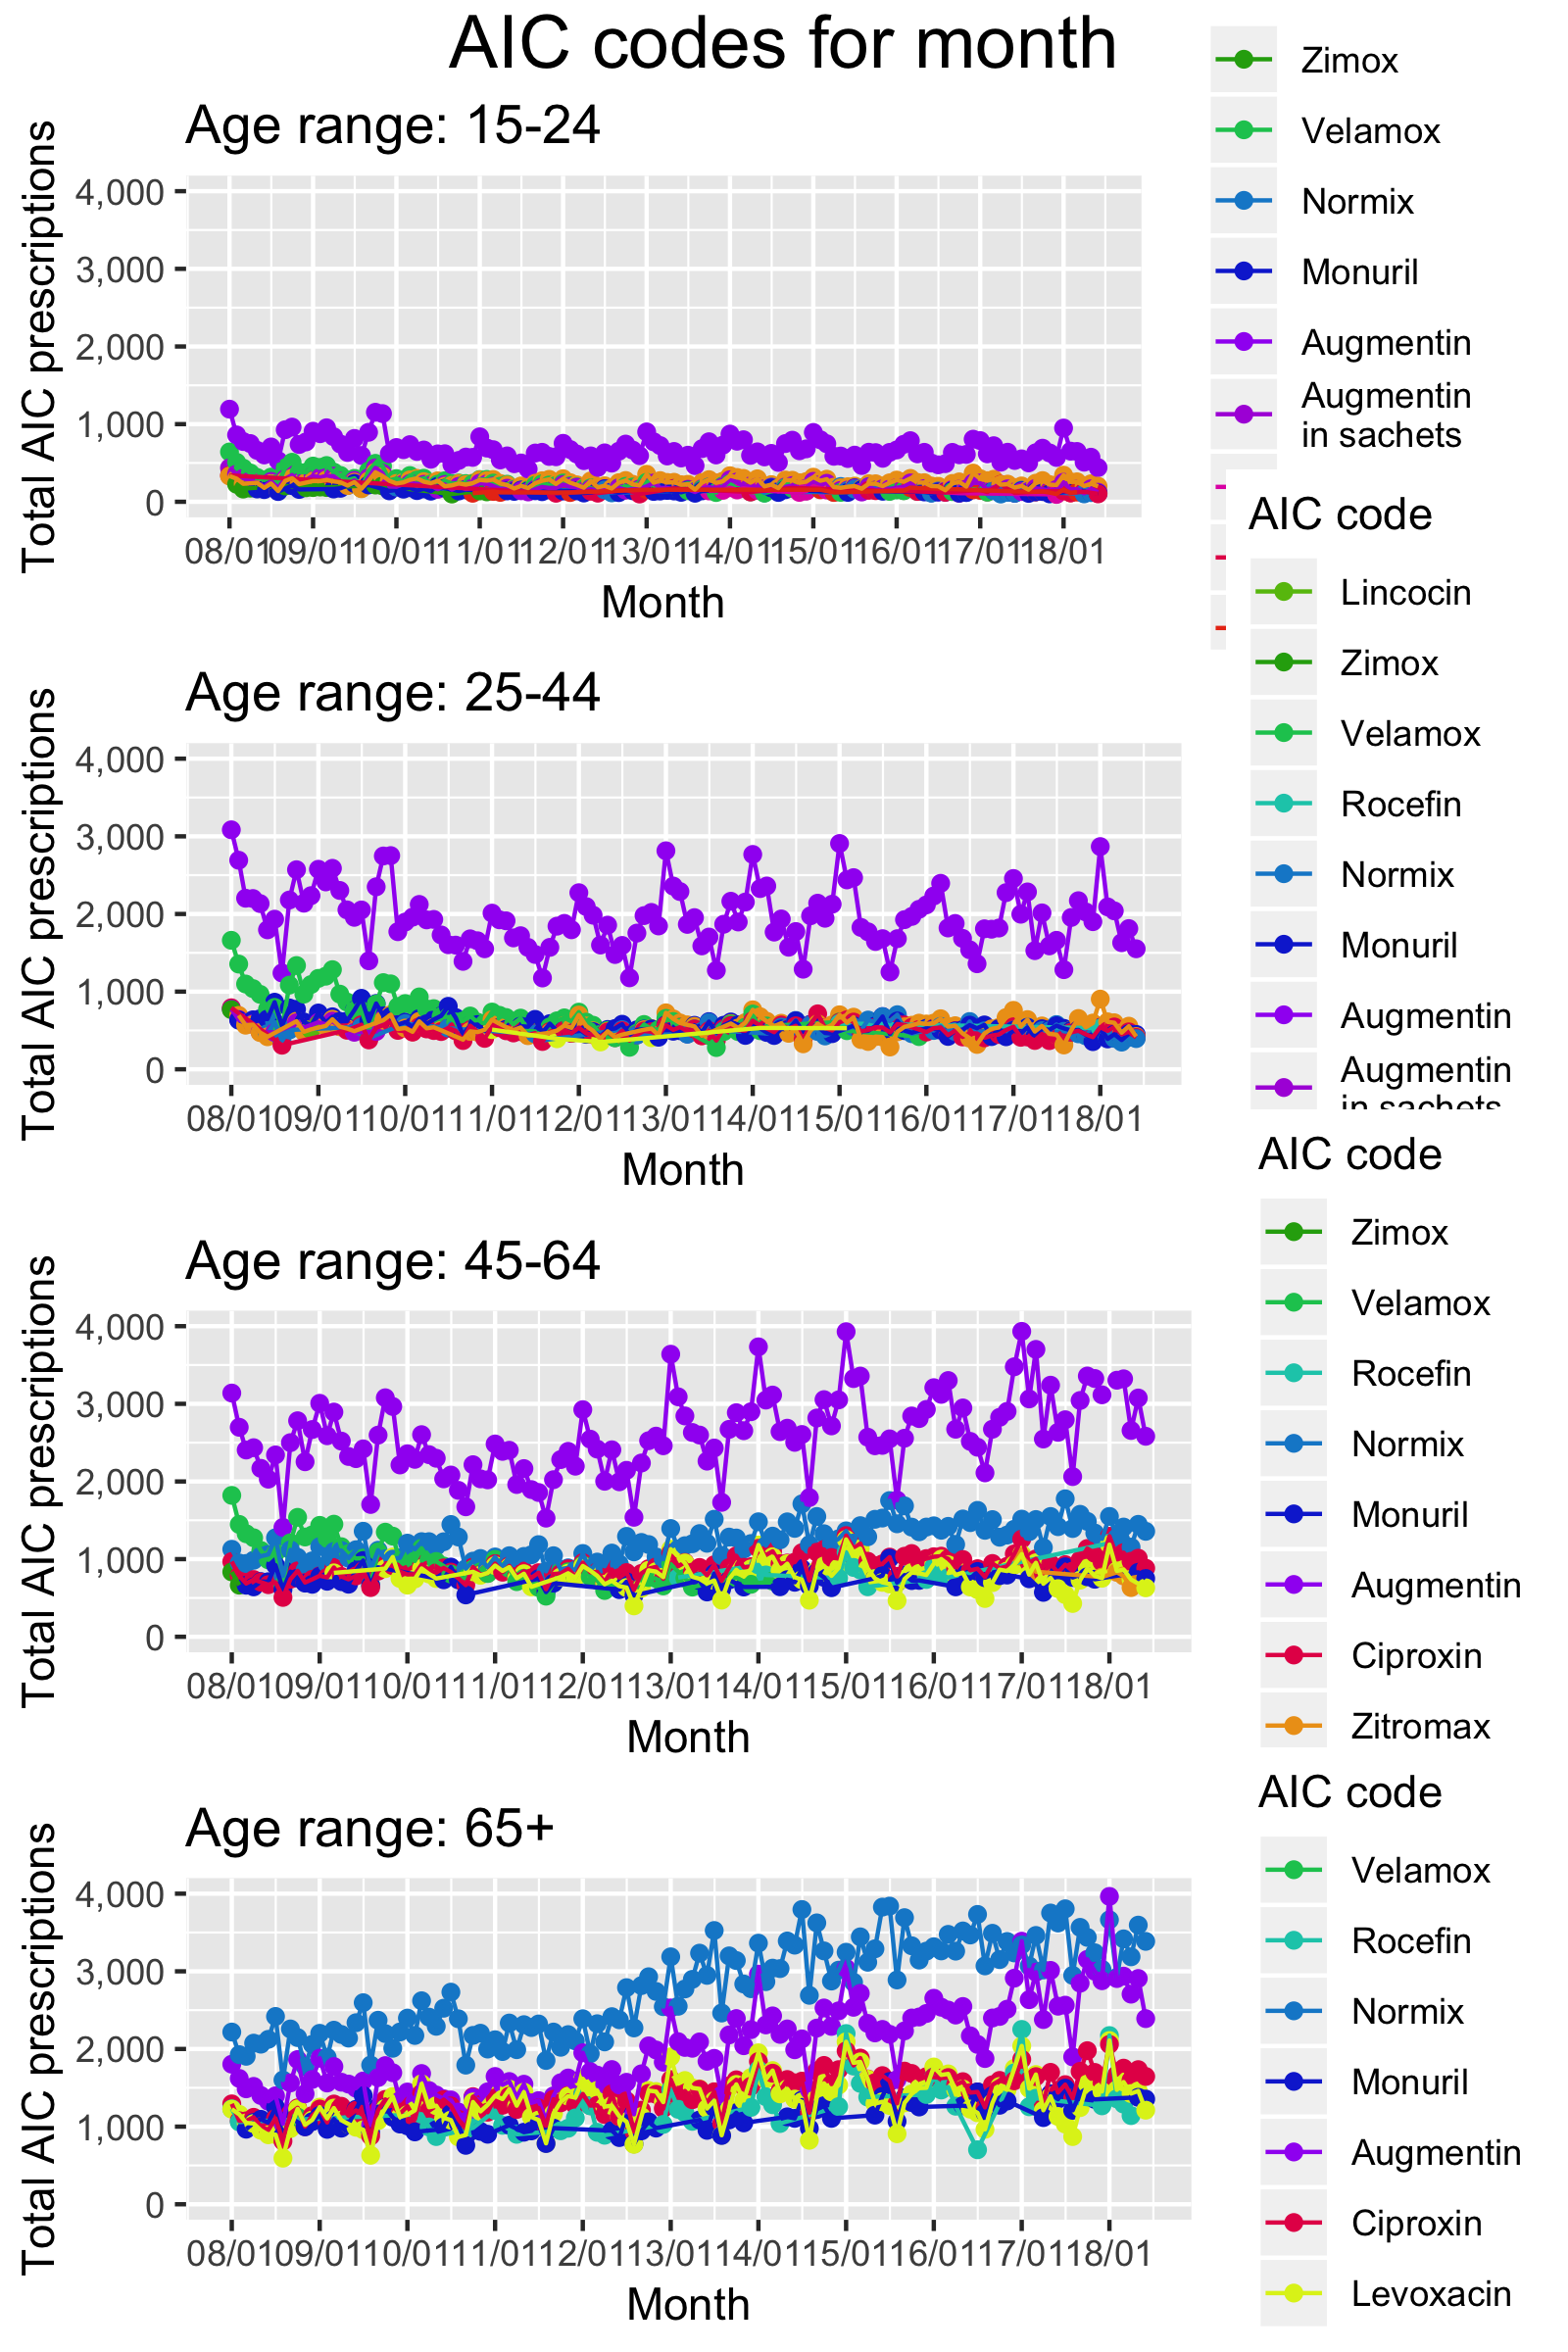
\includegraphics[scale=0.29]{../plots/top_aic_age-month.png}
\end{figure}

\subsection{ATC and AIC correlation}

 % finire analitiche sul sesso, sistemare grafici età, analitiche icd9-atc
\chapter[k-means approach]{\textit{k}-means approach for cluster analysis}
This chapter illustrates the implementations of the $k$-mean algorithm on a matrix of general practitioners and prescriptions for antibiotic, to classify them according to their behaviour.

\textbf{\textit{k}-means clustering} is the most commonly used unsupervised machine learning algorithm for dividing a given dataset into $k$ clusters. 

This method related to antibiotic resistance research consists in applying a time series clustering approach to \textit{group general practitioners according to their prescriptive habits of antibiotics}, using medicines as profiling instrument to obtain models of usage for each product.

Additional layers (factors) to consider while profiling are space, time, structure and personal information of patients, to highlight potential behaviours to classify doctors and co-prescription activities. 

Data has therefore to be subject of parsing, grouping values b to chosen features and selecting subsets based on consistency, maximising potential given information. 

Records will be mapped into a $n$-dimensional matrix which will be fed to the algorithm, obtaining a cluster of belonging for each element. Dimensions will represent \textbf{individuals}, \textbf{relevant features} and \textbf{time}, yet time slices will be taken separately to be able to make comparisons and predictions. 

Results aim to identify whether general practitioners are ``loyal'' prescribers: having most prescribed antibiotics, checking whether there exist typologies of patterns according to active and illustrative variables. 

$k$-means is the chosen clustering algorithm, since the approach is non-hierarchical and simple: its minimum computation complexity and ease of use make it the most suitable algorithm to perform an initial clustering on raw data, reducing the space into disjoint smaller sub-spaces to then perform additional analysis.

After identifying the clusters and linking each one with a specific prescription patten, it is possible to discriminate between GPs with \textit{changing} and \textit{constant} behaviours among time.

\section{Range of time}
Since the aim of clustering is identifying prescription patterns and their changes, extracting \textbf{different time slices} allows better insights on evolutions of trends.

To avoid the impact of seasonality, having values increasing in the winter months, data is collected and aggregated in a range of \textbf{one year}: the final table contains cumulative results and features, without distinction between different times of the year.

Comparisons are made selecting two snapshots of data according to different years, and visualising outcomes to understand whether values have shifted cluster (general practitioners have changed habits).

Data in two years needs to be distant enough to ensure the presence of potential changes, yet consistent enough to prevent information loss. 

Selected years are \textbf{2010} and \textbf{2017}, 2017 being the latest complete time range and 2010 being the first year considered for antibiotics analysis.

\section{Dataset construction}
Before being able to apply a clustering algorithm, data has to be cleaned, arranged and aggregated: having a format of single prescription records would not give the desired outcome, since grouping has to be made according to \textit{counts in years}.

\textbf{Transposing} information from a row to a column visualisation allows to emphasise the values of each feature.

The most important constraint while constructing the matrix is consistency of data: all general practitioners must be active in both years, to make comparison possible.

The number of constantly active doctors is 372, having respectively 228 022 and 214 316 patients in 2010 and 2017. This implies a data loss of about 75\% in both sets.

Features to consider are:
\begin{itemize}
	\item Antibiotic prescriptions;
	\item Patients data;
	\item Other prescriptions' habits data.
\end{itemize}

To limit horizontal expansion of the matrix, a limited number of attributes are taken into account, chosen by their relevancy:
\begin{itemize}
	\item Antibiotic prescriptions are broken and counting according to the \textbf{8 most popular products} (Augmentin, Normix, Ciproxin, Levoxacin, Monuril, Velamox, Rocefin, Zitromax);
	\item Patients data only includes \textbf{gender} and most common \textbf{age range} in $\{1, 2, 3, 4\}$. 
\end{itemize}

Other prescriptions' data has been limited to the \textit{total number of prescriptions} (not strictly related to antibiotics) for each year. Information about the total amount of prescriptions might be helpful to understand the percentage of antibiotics respecting to the whole, and therefore their influence.

According to the goal of the analysis, every sample is represented as a \textbf{13-dimensional vector}, with each row containing information on a single general practitioner.

Displayed below is an extract of the final table for 2017:
\begin{center}
	\begin{table}[h]
	 \makebox[\textwidth][c]{
	\begin{tabular}{c|c|c|c|c|c|c|c|c}
		\textbf{\#} & \textbf{Doctor ID} & \textbf{Aug.} & \textbf{Normix} & \dots & \textbf{M. patients} & \textbf{F. patients} & \textbf{Age} & \textbf{Prescriptions} \\
		\hline
		1 & DRTQRGJ & 5 & 123 & \dots & 303 & 397 & 3 & 17 862 \\
		\hline 2 & DSJRY7B & 242 & 131 & \dots & 322 & 399 & 4 & 15 845 \\
	\end{tabular}}
\caption{\small $k$-means matrix extract}
\vspace{-20px}
\end{table}
\end{center}

Input matrix has dimensions of $372 \times 13 \times 2$, where the latter is an additional time dimension which distinguishes between 2000 and 2017, removed splitting the dataset to run the algorithm separately in the two years.

\section{Features selection}
Having too many features, despite the initial grouping, may lead to overfitting and having general practitioners clustered according to irrelevant information.

Among all features, some are relevant for the outcome of the algorithm, while others are purely descriptive to be checked after clustering results.

All the amounts of \textit{prescriptions} for each antibiotic (columns 1-9) have to be considered to extract similarity, and scaled to normalise numbers. Those count as \textbf{active variables}, and clustering will be performed considering the subset of belonging.

Doctors' IDs are removed during computation, to then be added back to map each row with its belonging individual. 

The other attributes are \textbf{illustrative}, and will be attached to clustering results, to offer further information to be compared after having a general idea of each doctor's group. 

\section{Optimal number of clusters}
Determining the most suitable number of clusters in a data set is a fundamental issue in $k$-means clustering, which requires the user to specify the number of clusters $k$ to be generated. There are various approaches to pick the best value, yet the method is ultimately subjective\cite{silhouette}.

\subsection{\texttt{NbClust}}
\texttt{NbClust} is a R package which provides 30 indices for determining the number of clusters and proposes the best clustering scheme from the different results obtained by varying all combinations of number of clusters, distance measures, and clustering methods. 

Both datasets have been tested with \texttt{NbClust} using number of clusters in $\{2, 20\}$.

Results for 2010:
\begin{lstlisting}
* Among all indices:                                                
* 8 proposed 2 as the best number of clusters 
* 2 proposed 3 as the best number of clusters 
* 1 proposed 7 as the best number of clusters 
* 7 proposed 8 as the best number of clusters 
* 1 proposed 12 as the best number of clusters 
* 1 proposed 14 as the best number of clusters 
* 2 proposed 15 as the best number of clusters 
* 1 proposed 20 as the best number of clusters 

***** Conclusion *****                            

* According to the majority rule, the best number of clusters is  2 
\end{lstlisting}

Results for 2017:
\begin{lstlisting}
* Among all indices:                                                
* 9 proposed 2 as the best number of clusters 
* 1 proposed 3 as the best number of clusters 
* 1 proposed 6 as the best number of clusters 
* 3 proposed 9 as the best number of clusters 
* 1 proposed 14 as the best number of clusters 
* 1 proposed 15 as the best number of clusters 
* 1 proposed 18 as the best number of clusters 
* 2 proposed 19 as the best number of clusters 
* 5 proposed 20 as the best number of clusters 

***** Conclusion *****                            

* According to the majority rule, the best number of clusters is  2 
\end{lstlisting}

It can be seen that indices give 2 as optimal number of clusters for both matrices.

\subsection{Elbow and silhouette}
Direct methods consist in optimizing a criterion, such as the within cluster sums of squares or the average silhouette. The corresponding methods are named elbow and silhouette methods, respectively.

A detailed trend on the optimal number of clusters can be obtained applying respectively the WSS (Within Sum of Squares) and silhouette indexes in R.

The basic idea behind partitioning methods is to define clusters such that the total intra-cluster variation (or total within-cluster sum of square, WSS) is minimized. The total WSS measures the compactness of the clustering, which should be as small as possible.

The Elbow method looks at the total WSS as a function of the number of clusters: one should choose a number of clusters so that adding another cluster doesn't improve much better the total WSS.

Average silhouette method computes the average silhouette of observations: it measures how similar a sample is to the others belonging to the same cluster, compared to how similar it is to the others in different clusters, estimating the distance between clusters for different values of $k$.

The optimal number of clusters $k$ is the one that maximize the average silhouette over a range of possible values\cite{silhouette}.

\begin{figure}[h]
	\centering
	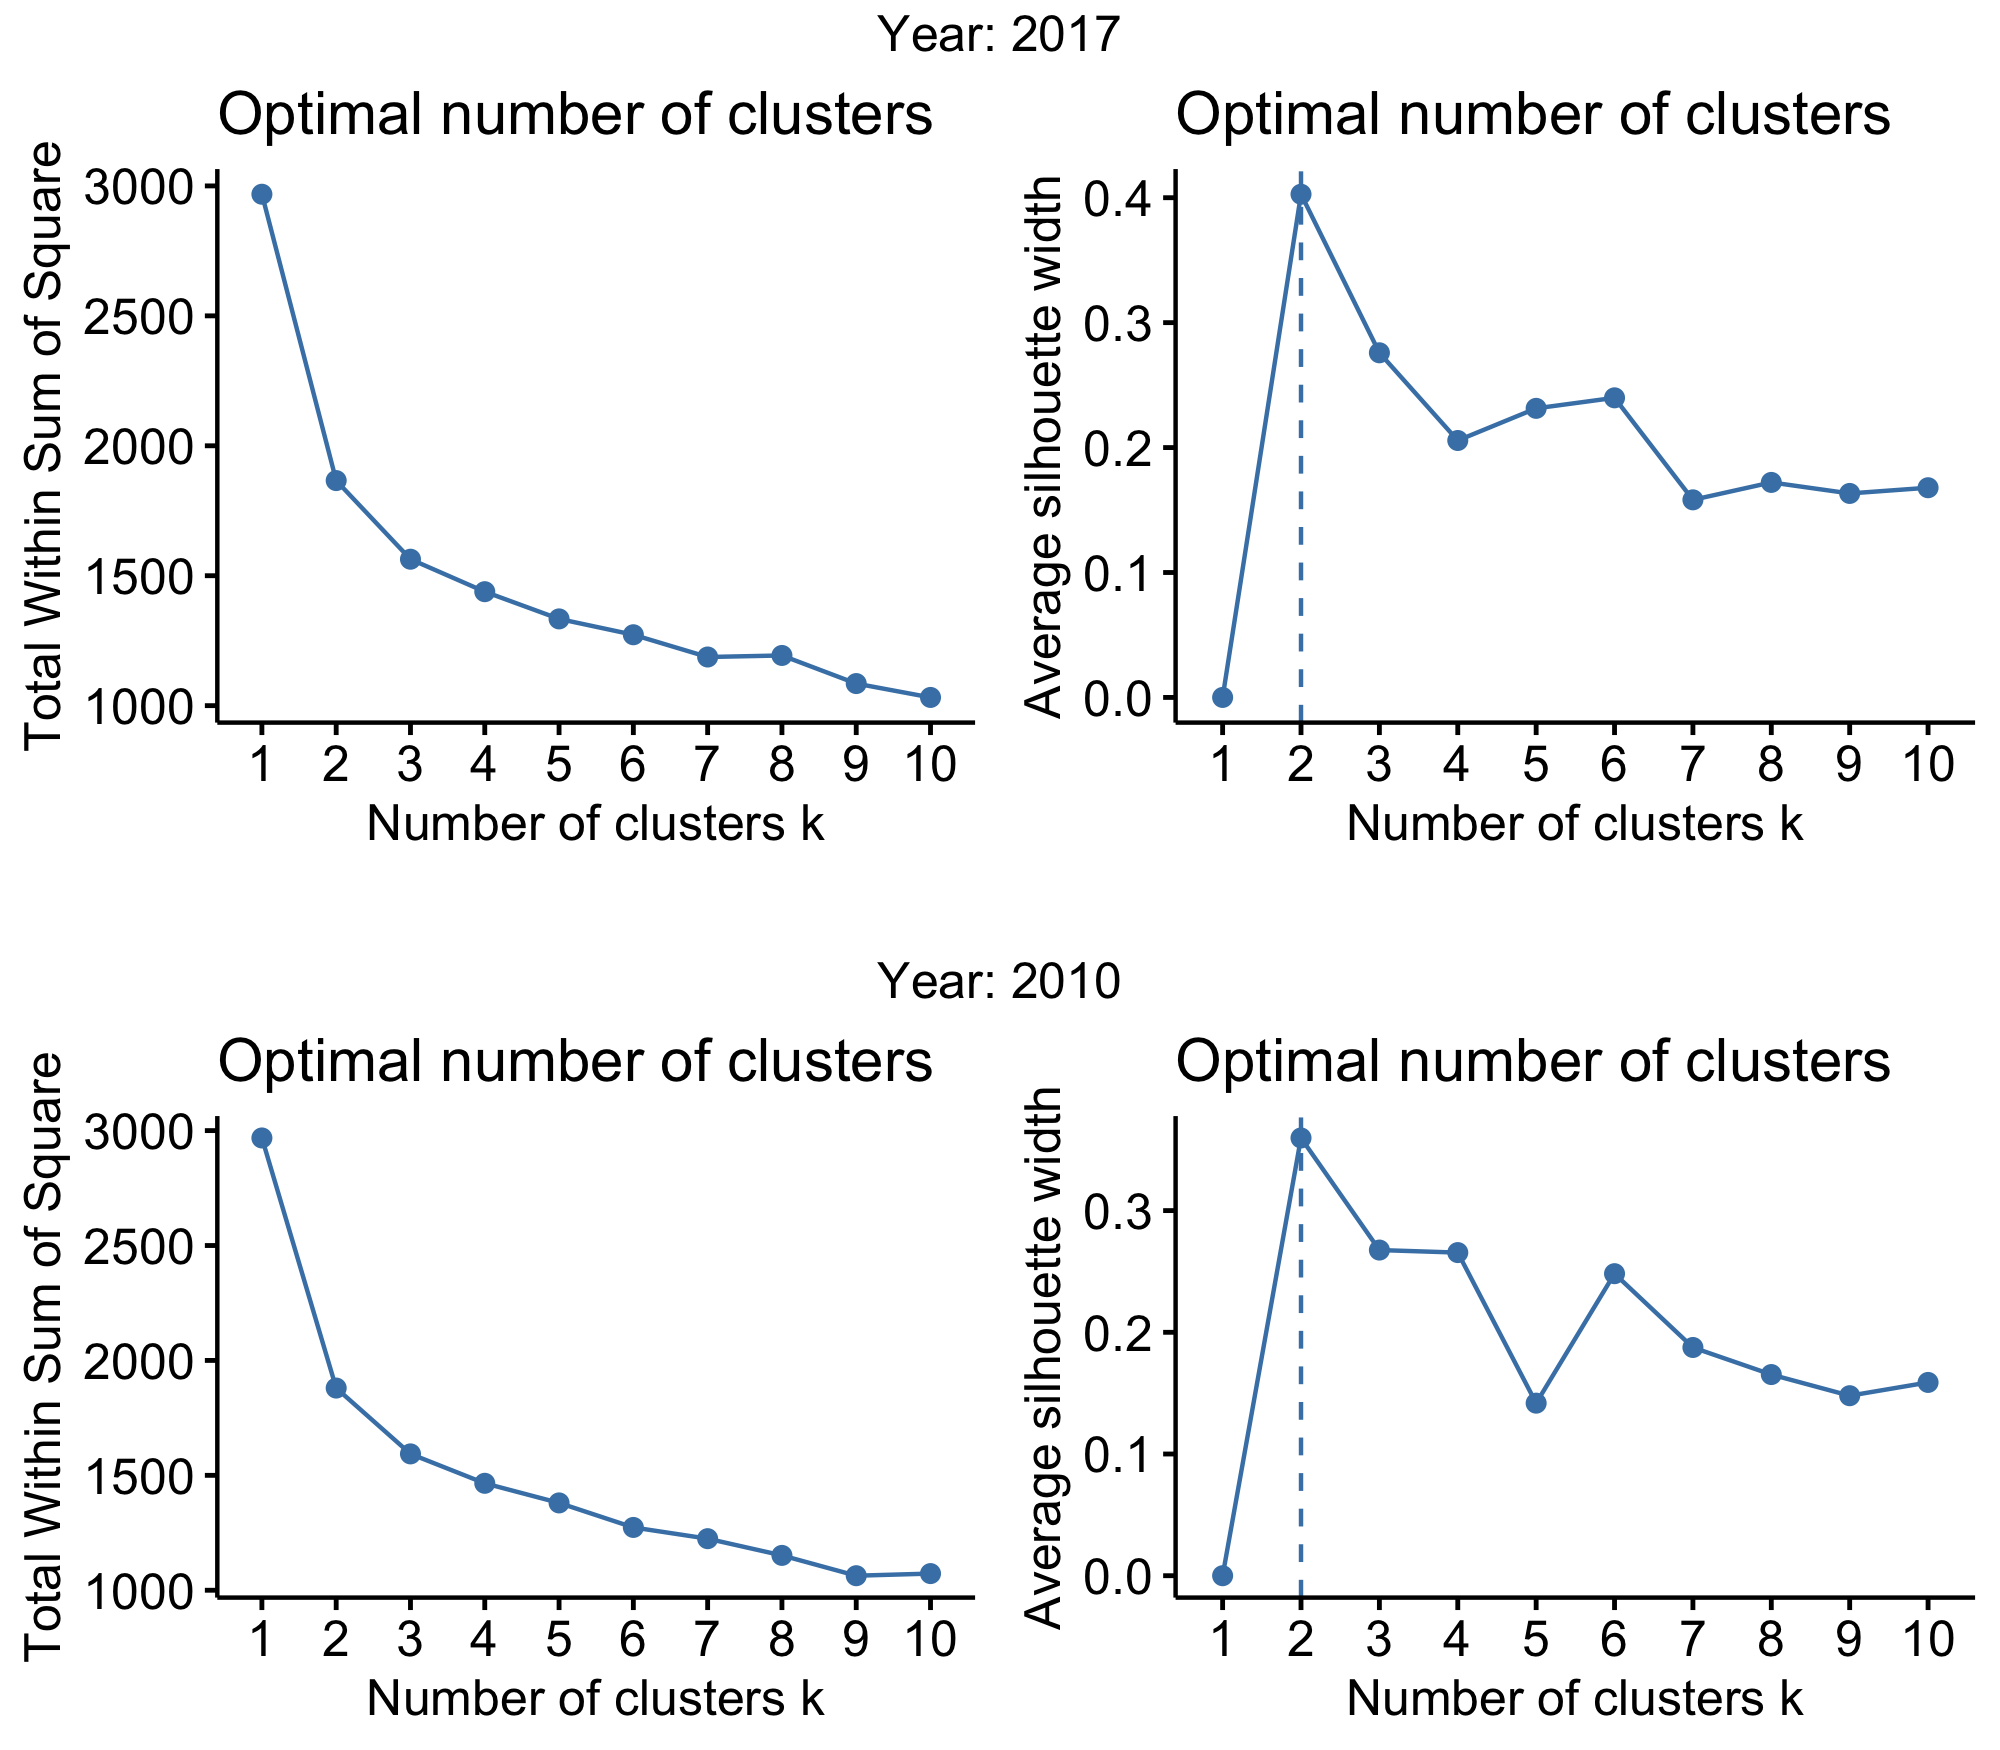
\includegraphics[scale=0.22]{../k-means/optimal-clusters.png}
	\caption{\small WSS and silhouette indexes for $k$-means}
\end{figure}

It can be seen in the figure that both indexes show 2 as the best number, coherently with \texttt{NbClust}, yet 5 or 6 clusters give an acceptable score as well.

Having 2 clusters increases the risk of classification according to \textbf{irrelevant features}, such as large and small prescribers, giving no other useful information.

Therefore, the algorithm is subject of an \textbf{additional run} with an arbitrary amount of 4 clusters, observing how many individuals compose each cluster and eventually adjusting the value of $k$.

\section{Results}

\subsection{2 clusters} 

\subsubsection{Year 2010}
\begin{center}
	\begin{table}[h]
	\makebox[\textwidth][c]{
		\begin{tabular}{c|c|c|c|c|c|c|c|c|c}
			\textbf{\#} & \textbf{Augmentin} & \textbf{Normix} & \textbf{Ciproxin} & \textbf{Levox.} & \textbf{Mon.} & \textbf{Vel.} & \textbf{Roc.} & \textbf{Zitr.} & \textbf{Size} \\
			\hline
			1 & 64,44 & 52,95 & 36,96 & 37,39 & 32,23 & 34,45 & 25,88 & 25,15 & 232 \\
			\hline
			2 & 224,59 & 131,29 & 86,29 & 80,10 & 80,25 & 99,74 & 62,08 & 54,15 & 140 \\
	\end{tabular}}
\caption{\small $k$-means with 2 clusters, 2010}
\vspace{-30px}
\end{table}
\end{center}
\medskip

\subsubsection{Year 2017}
\begin{center}
	\begin{table}[h]
	\makebox[\textwidth][c]{
		\begin{tabular}{c|c|c|c|c|c|c|c|c|c}
			\textbf{\#} & \textbf{Augmentin} & \textbf{Normix} & \textbf{Ciproxin} & \textbf{Levox.} & \textbf{Mon.} & \textbf{Vel.} & \textbf{Roc.} & \textbf{Zitr.} & \textbf{Size} \\
			\hline
			1 & 95,69 & 70,46 & 49,27 & 42,37 & 37,51 & 21,74 & 36,17 & 32,14 & 242 \\
			\hline
			2 & 316,50 & 185,61 & 104,90 & 86,72 & 89,07 & 42,25 & 77,11 & 79,42 & 130 \\
	\end{tabular}}
\caption{\small $k$-means with 2 clusters, 2017}
\vspace{-30px}
\end{table}
\end{center}
\medskip

\subsubsection{Considerations}
The two clusters have a consistent different between the \textbf{means} of antibiotic prescriptions' amounts, especially Augmentin and Velamox, which are the most popular. 

This leads to considering two clusters as \textit{heavy} prescribers and \textit{light} ones, as expected.

Comparison between total prescriptions of members of each cluster:
\begin{table}[h]
	\centering
	\begin{tabular}{c|c|c|c}
		\textbf{Year} & \textbf{Cluster} & \textbf{Mean} & \textbf{SD} \\
		\hline
		2010 & 1 & 9 043,41 & 5 120,81 \\
		\hline
		2010 & 2 & 18 228,35 & 5 314,28 \\
		\hline
		2017 & 1 & 10 126,52 & 5 392,88 \\
		\hline
		2017 & 2 & 19 755,14 & 5 360,95 \\
	\end{tabular}
\caption{\small Comparison of total prescriptions within clusters}
\end{table}

Standard deviation of total amount of prescription is overall the same, which implies clustering has consistent and related results. Mean between first and second cluster tends to increase during the years, yet is still close.

This confirms the hypothesis of grouping according to the number of prescriptions.

The amount of general practitioners in the clusters is almost the same from 2010 to 2017, with 78 doctors swapping clusters in total:
\begin{itemize}
	\item 44 switched from large prescribers to small ones;
	\item 34 switched from small prescribers to large ones.
\end{itemize}
The difference of 10 switching doctors is the same as the difference between cluster 1 in 2010 and cluster 1 in 2017.

General practitioners overall remained mostly stable with their amount of prescriptions, yet some switched habits while the mean of total prescriptions increased. This most likely implies that doctors classified as large prescribers still consistently increased their numbers, so that the mean grew by roughly 1 000 in 7 years, although some doctors started to prescribe less.

Clusters for each year are shown performing a PCA among the considered features (number of prescriptions for each antibiotic) with the \texttt{fviz\_cluster} function from package \texttt{factoextra}. 

\begin{figure}[h]
	\centering
	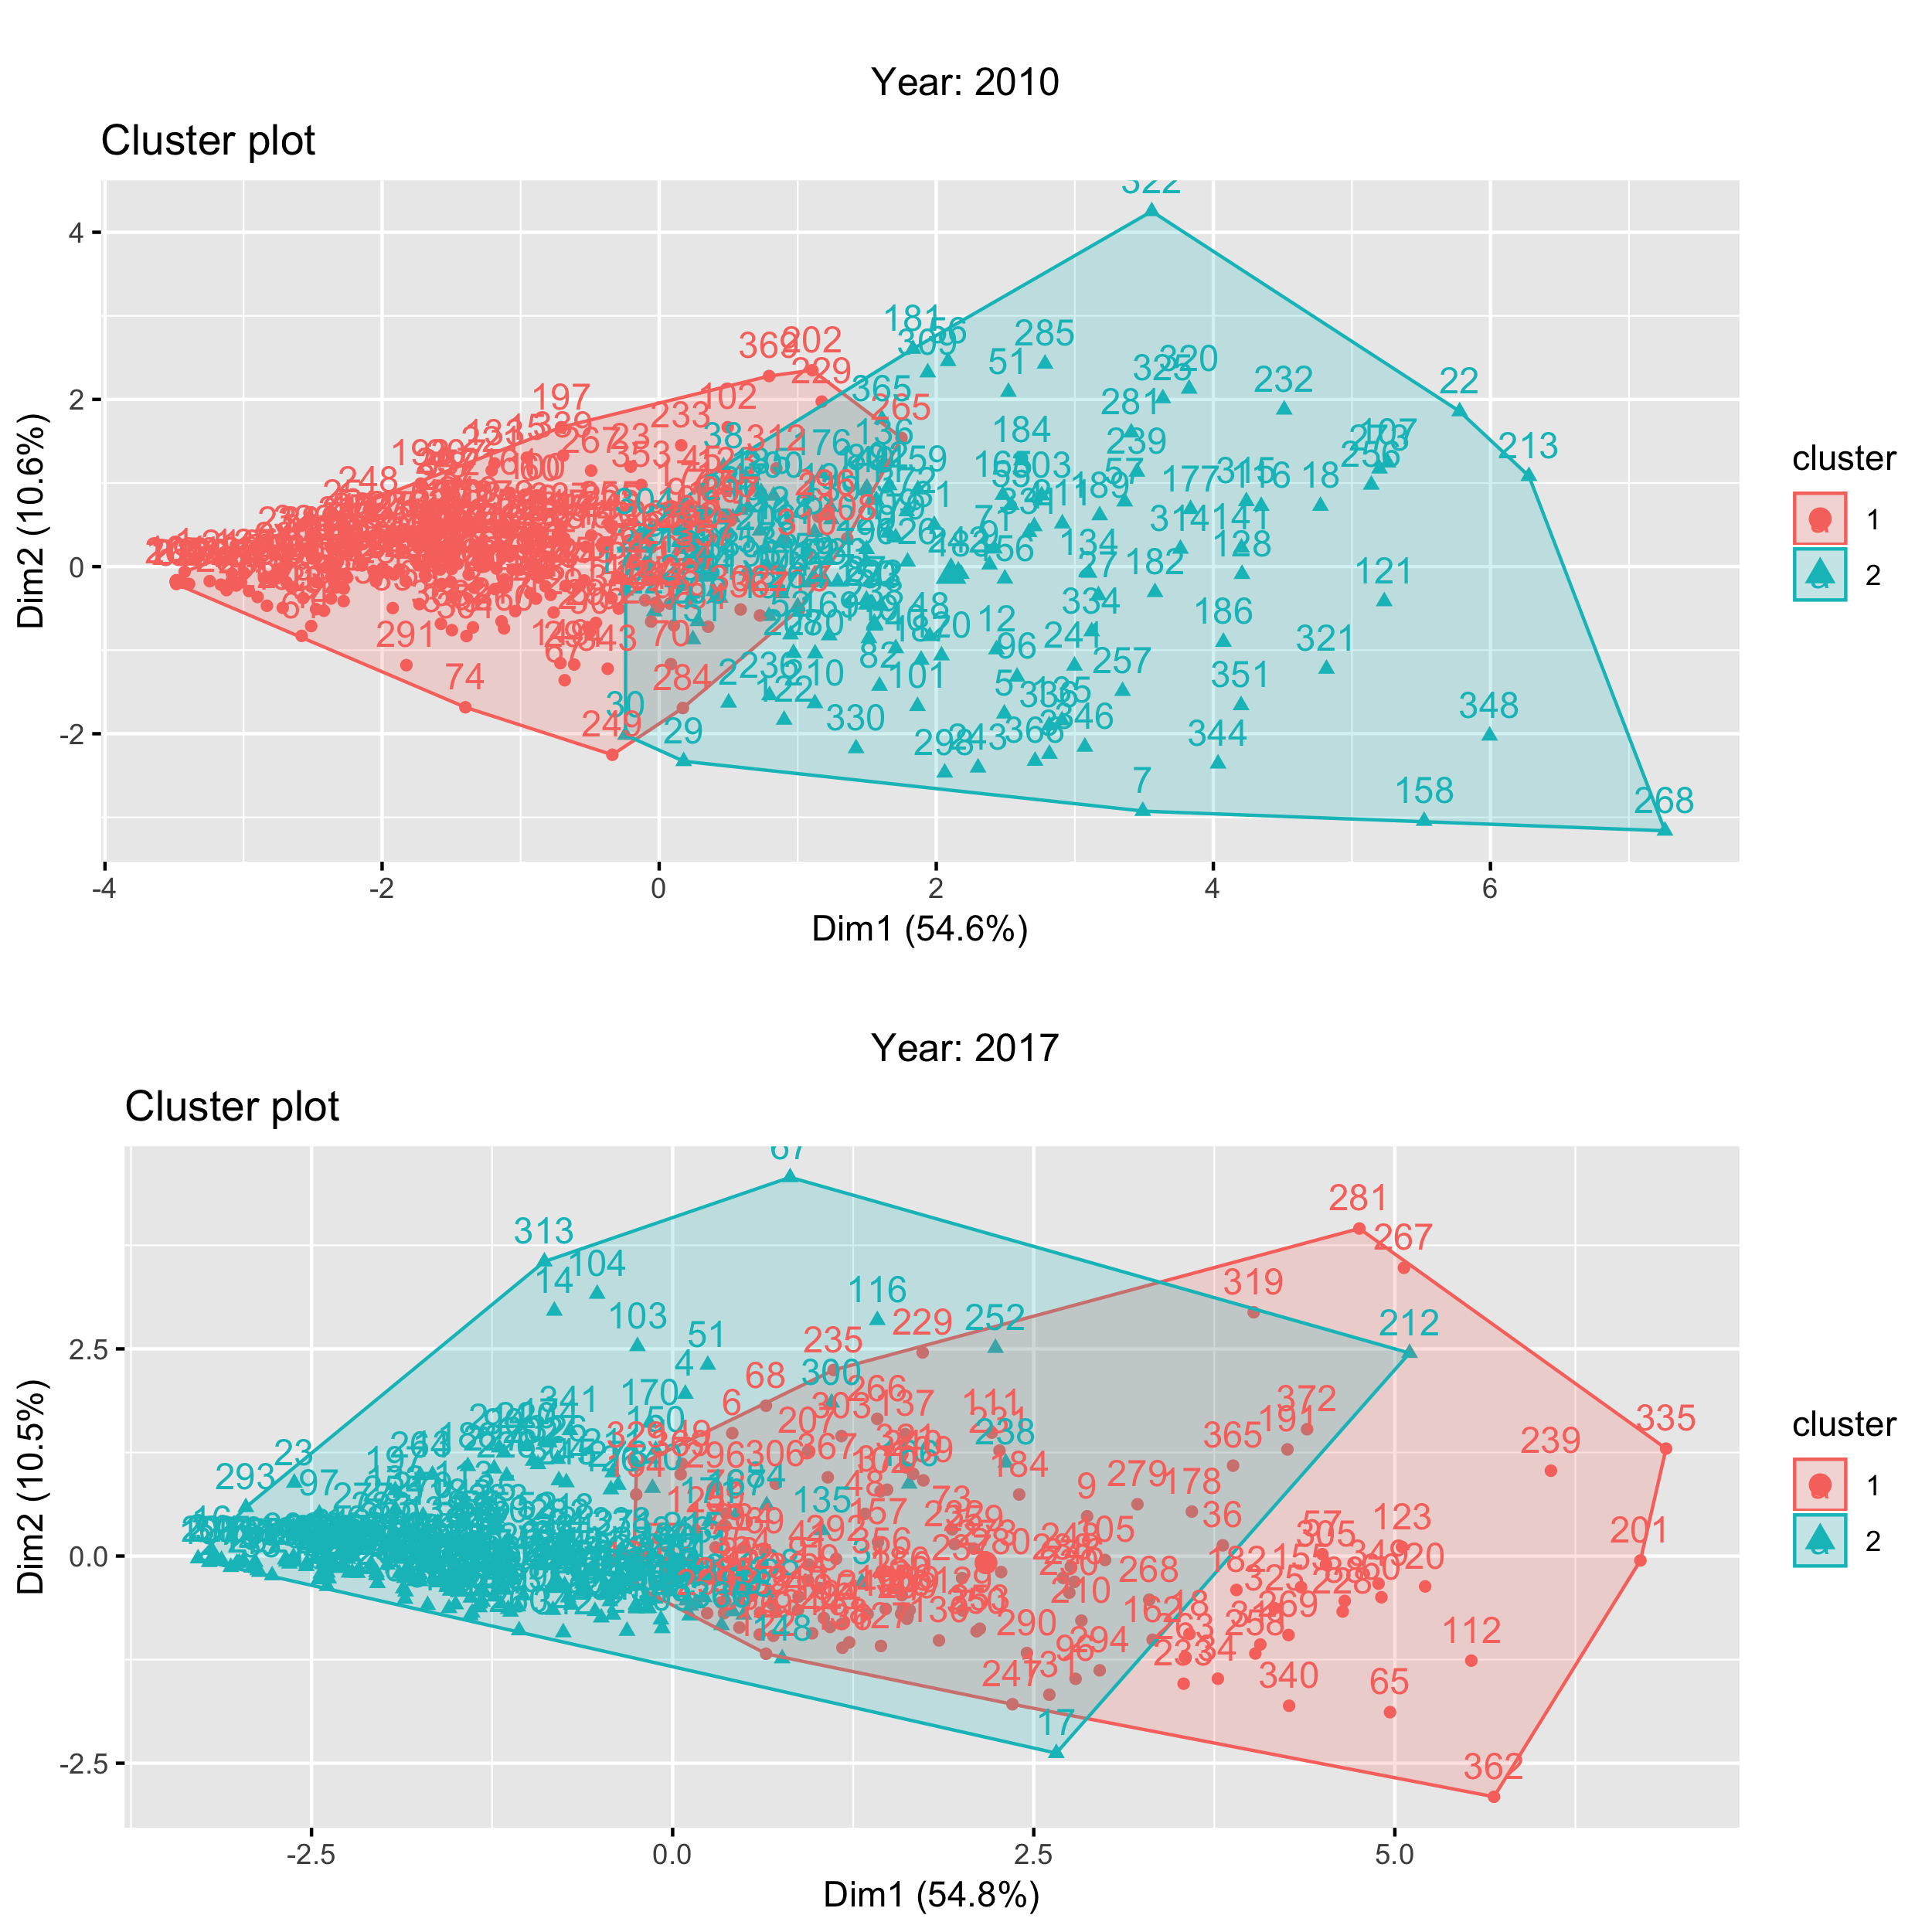
\includegraphics[scale=0.18]{../k-means/clusters-2.png}
	\caption{\small PCA with 2 clusters}
\end{figure}

Each number represents the row corresponding to a general practitioner, while the axes are principal components. Clusters tend to overlap because of the dimensionality reduction.

\subsection{4 clusters}

\subsubsection{Year 2010}
\begin{center}
	\begin{table}[h]
 \makebox[\textwidth][c]{
		\begin{tabular}{c|c|c|c|c|c|c|c|c|c}
			\textbf{\#} & \textbf{Augmentin} & \textbf{Normix} & \textbf{Ciproxin} & \textbf{Levox.} & \textbf{Mon.} & \textbf{Vel.} & \textbf{Roc.} & \textbf{Zitr.} & \textbf{Size} \\
			\hline
			1 & 291,35 & 187,93 & 107,84 & 94,42 & 102,02 & 159,28 & 70,68 & 65,37 & 45 \\
			\hline
			2 & 86,85 & 120,96 & 68,14 & 70,03 & 65,63 & 76,75 & 48,13 & 47,63 & 61 \\
			\hline
			3 & 195,29 & 85,38 & 69,41 & 61,93 & 61,60 & 57,77 & 50,10 & 43,20 & 103 \\
			\hline
			4 & 48,27 & 37,02 & 27,59 & 30,61 & 23,15 & 25,51 & 20,97 & 19,14 & 163 \\
	\end{tabular}}
\caption{\small $k$-means with 4 clusters, 2010}
\vspace{-30px}
\end{table}
\end{center}
\medskip

\subsubsection{Year 2017}
\begin{center}
	\begin{table}[h]
	\makebox[\textwidth][c]{
		\begin{tabular}{c|c|c|c|c|c|c|c|c|c}
			\textbf{\#} & \textbf{Augmentin} & \textbf{Normix} & \textbf{Ciproxin} & \textbf{Levox.} & \textbf{Mon.} & \textbf{Vel.} & \textbf{Roc.} & \textbf{Zitr.} & \textbf{Size} \\
			\hline
			1 & 397,54 & 236,54 & 124,08 & 101,05 & 107,93 & 55,01 & 87,51 & 112,71 & 59 \\
			\hline
			2 & 32,57 & 165,30 & 89,50 & 90,31 & 76,88 & 47,65 & 72,69 & 69,80  & 26 \\
			\hline
			3 & 228,18 & 119,93 & 78,85 & 63,74 & 63,15 & 28,99 & 59,01 & 46,01 & 117 \\
			\hline
			4 & 78,24 & 52,33 & 39,33 & 33,88 & 28,84 & 16,92 & 28,36 & 25,03 & 170 \\
	\end{tabular}}
\caption{\small $k$-means with 4 clusters, 2017}
\vspace{-30px}
\end{table}
\end{center}

\subsubsection{Considerations}
According to the cluster means for each antibiotic, general practitioners within clusters can be classified as:
\begin{enumerate}
	\item Large prescribers;
	\item Strong preference for Normix;
	\item Strong preference for Augmentin;
	\item Small prescribers.
\end{enumerate}

It can be seen that Augmentin means for cluster 3 is higher than the Normix one for cluster 2: Augmentin is most likely the over-prescribed drug.

Similarities in clusters composition:
\begin{itemize}
	\item 28 doctors being large prescribers in 2010 stayed constant in 2017;
	\item 12 doctors being Normix prescribers in 2010 stayed constant in 2017;
	\item 55 doctors being Augmentin prescribers in 2010 stayed constant in 2017;
	\item 122 doctors being small prescribers in 2010 stayed constant in 2017.
\end{itemize}

Similarities show 20-40 doctors for each cluster switching prescription habits, with a total of 155 elements belonging to a different groups. Considering 372 original individuals, this consists in 41,6\%.

Cluster size varies, with cluster 2 being subject of a consistent decrease in the number of elements from 2010 to 2017, while all the others increase size. Normix prescribers, then, switched to another category.

Comparison between total prescriptions of members of each cluster:
\begin{table}[h]
	\centering
	\begin{tabular}{c|c|c|c}
		\textbf{Year} & \textbf{Cluster} & \textbf{Mean} & \textbf{SD} \\
		\hline
		2010 & 1 & 22 244,29 & 4 540,88 \\
		\hline
		2010 & 2 & 15 587,75 & 4 328,30 \\
		\hline
		2010 & 3 & 14 910,14 & 4 574,42 \\
		\hline
		2010 & 4 & 7 131,60 & 4 326,86 \\
		\hline
		2017 & 1 & 23 154,69 & 4 523,31 \\
		\hline
		2017 & 2 & 17 481,92 & 5 370,08 \\
		\hline
		2017 & 3 & 15 042,37 &4 699,17 \\
		\hline
		2017 & 4 & 8 459,83 & 4 601,97 \\
	\end{tabular}
	\caption{\small Comparison of total prescriptions within clusters}
\end{table}

Standard deviation tends to stay constant, and mean for large and small prescribers is widely different, therefore the predictions seem to be correct. Mean between Normix and Augmentin prescribers is similar, meaning that both general practitioners having this behaviour do not tend to overprescribe other medicines.

To have a detailed view of changes between Normix and Augmentin preferences, those groups are compared to each other and the major prescribers cluster:
\begin{itemize}
	\item 26 Normix prescribers in 2010 switched to Augmentin in 2017;
	\item 4 Augmentin prescribers in 2010 switched to Normix in 2017;
	\item 5 Normix prescribers in 2010 switched to large prescribers in 2017;
	\item 22 Augmentin prescribers in 2010 switched to large prescribers in 2017.
\end{itemize}

Normix prescribers progressively switched to large prescribers (cluster 1) or having Augmentin preference (cluster 3), and all Augmentin averages increased: in particular in cluster 1, those have an additional 100 prescriptions in 2017.

It is safe to assume that although small prescribers represent a considerable percentage of the total, Augmentin prescriptions are being pushed upwards, most likely because of antibiotic resistance and general practitioners' tendency to overprescribe.

Performing a run of the algorithm only using Augmentin and Normix values shows that, despite 2010 being the same, Normix prescriptions in 2017 aren't relevant enough to be the main characteristic of a cluster. 

Normix has therefore lost popularity within years: this is confirmed by antibiotics' trends graphs, showing a constant value for Normix prescriptions in the last years while Augmentin has a steady increase.

All the other antibiotics have constant trends as well, aside from the general raise from 2012 to 2015, yet values are consistently smaller, hence why the algorithm does not assess particular importance to them. 

Clusters for each year are again shown performing a PCA with \texttt{fviz\_cluster}.

\begin{figure}[h]
	\centering
	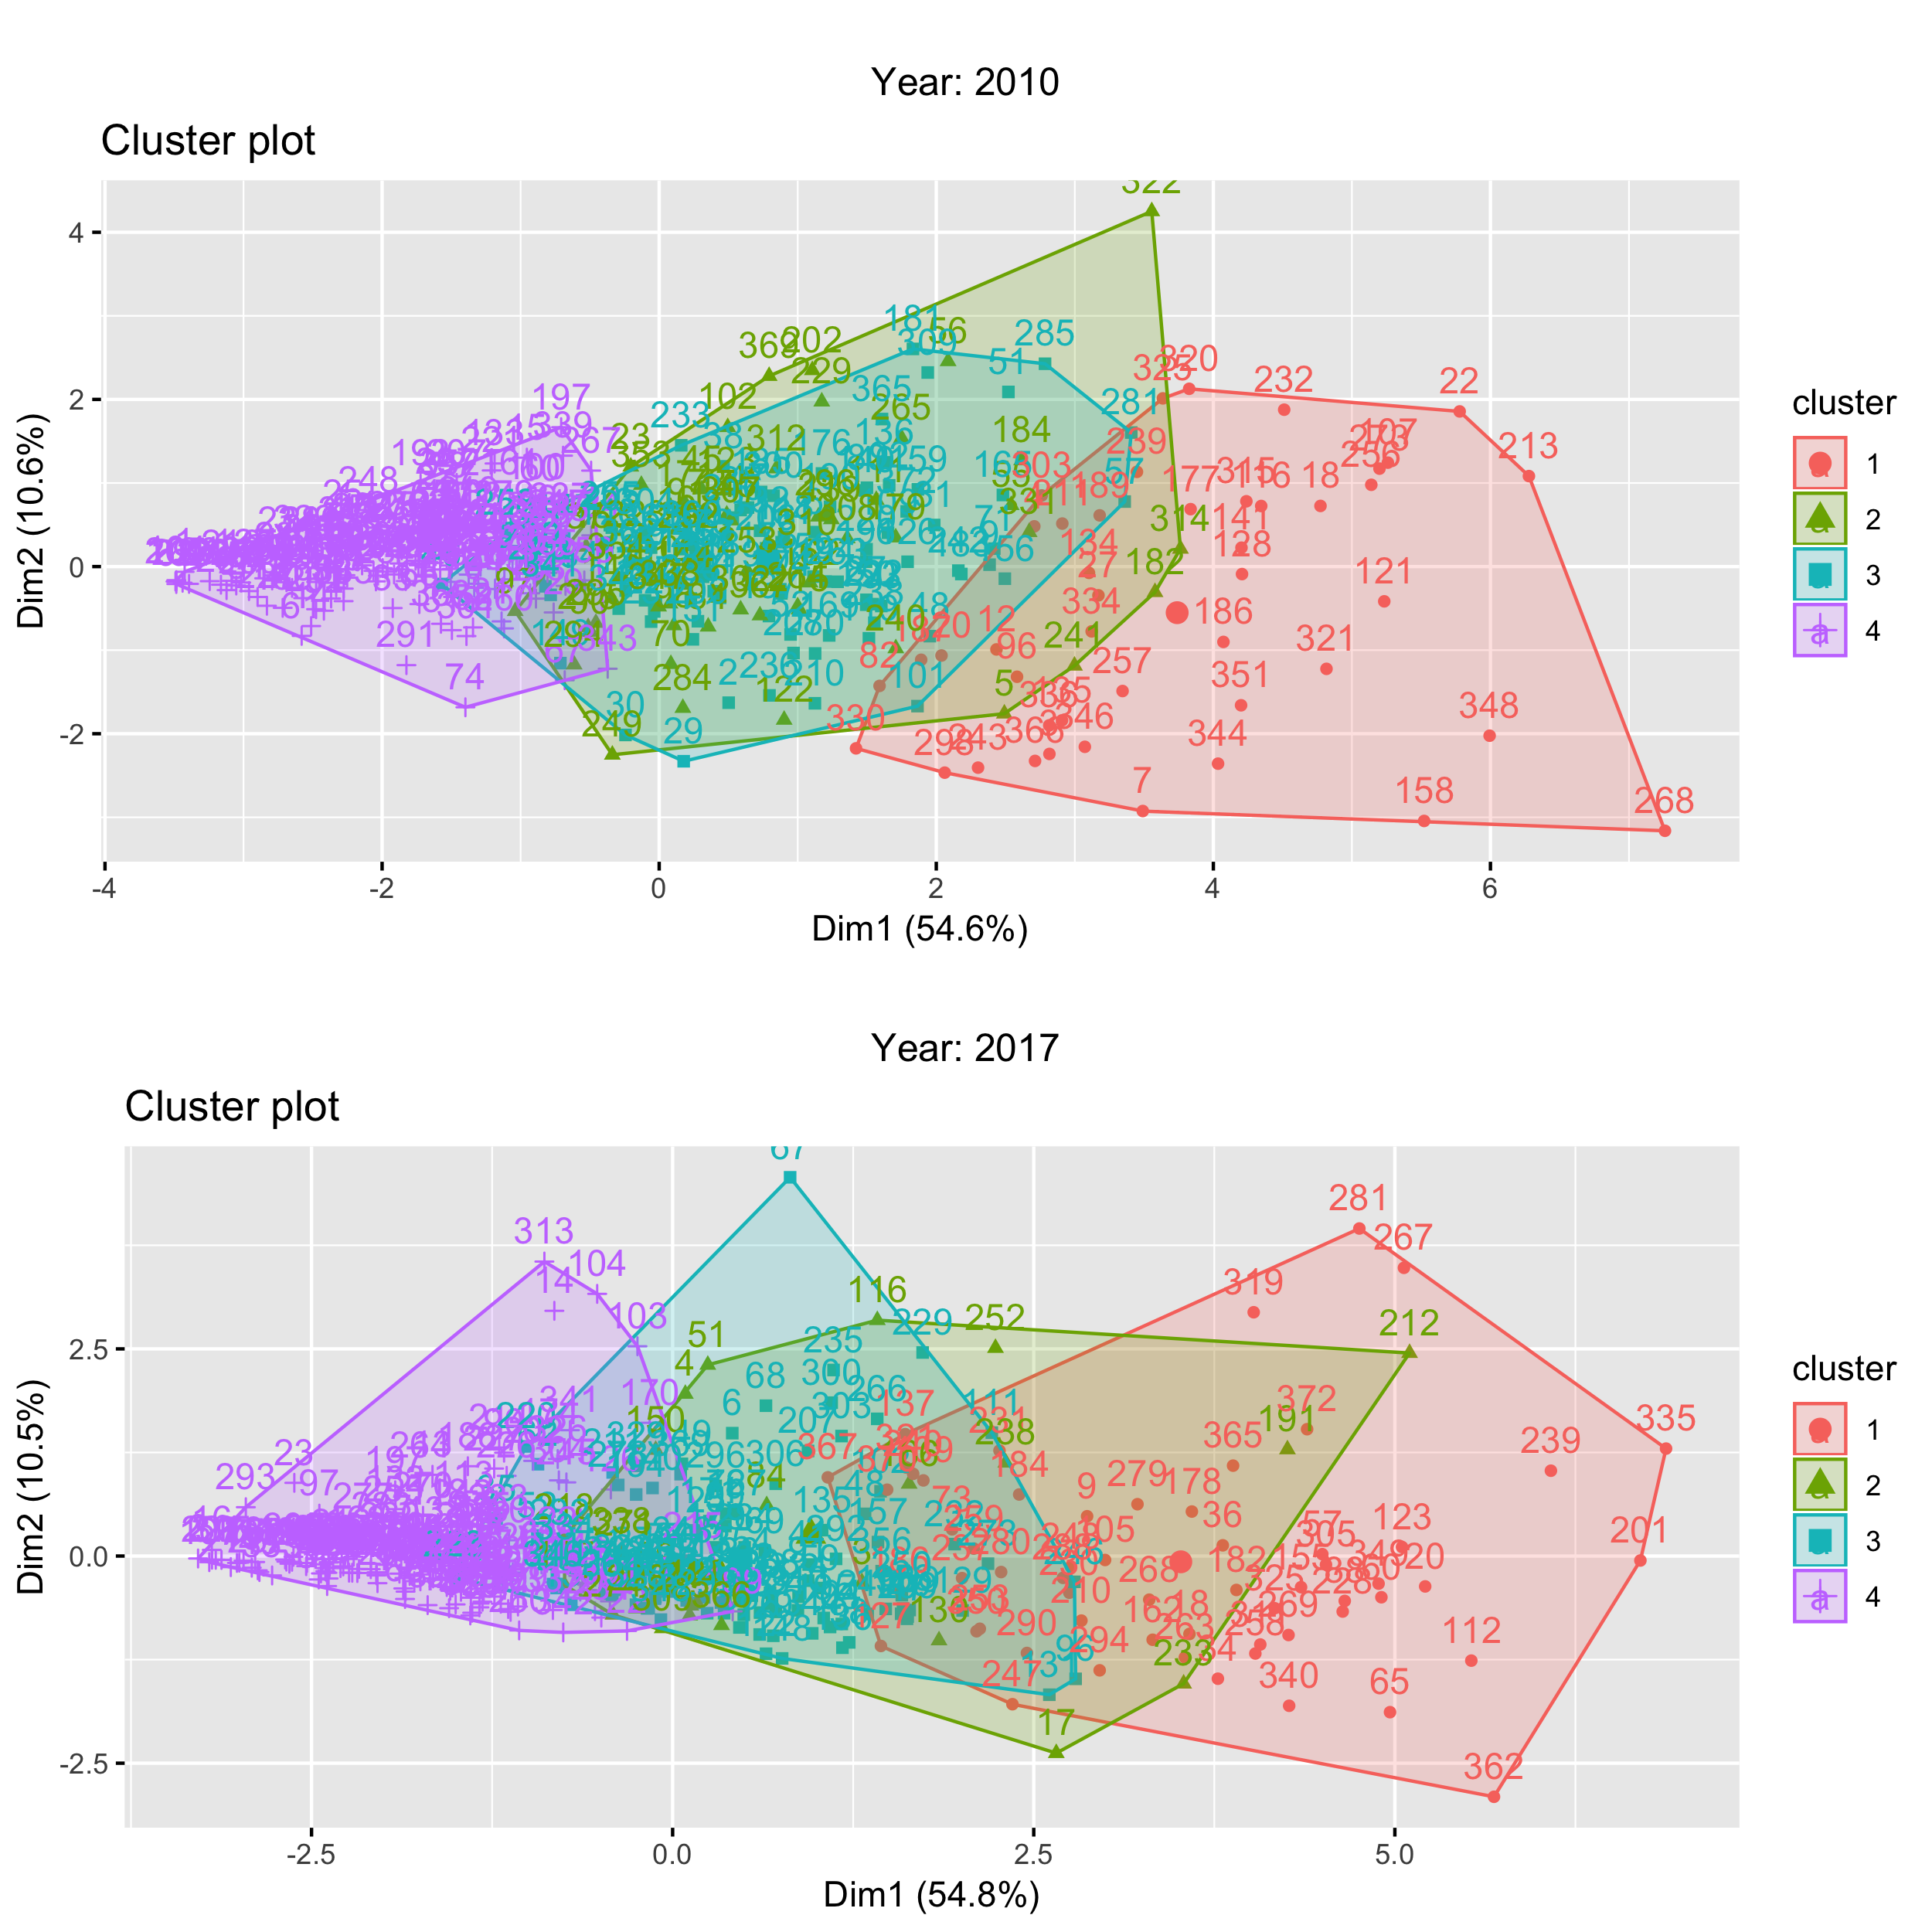
\includegraphics[scale=0.18]{../k-means/clusters-4.png}
	\caption{\small PCA with 4 clusters}
\end{figure}
 % tutto: costruzione della tabella, risultati, dimensioni, caratterizzati da che tipo di dati
% \chapter{Graph analysis}

\section{Prescription coupling}
An excessive usage of antibiotics causes death of microorganisms in the human body which provide to maintaining immune cells and killing certain oral infections\cite{bacteria}.

To equilibrate the intestinal flora, lactic ferments are often taken together with antibiotics, so that new ``good'' bacteria can restore the probiotic action.

If this hypothesis is correct, the dataset will show antibiotic prescriptions paired with other drugs, on the same date --- or it will highlight potential linkings between infections and other pathologies receiving a specific prescription.

\section{Graph databases}
Graph databases are data management systems allowing persistent representation of entity and relationship in a graph structure, implementing the Property Graph Model efficiently down to the storage level. % todo citare le slide di maurino

A graph $G\: =\: <E, V>$ is an abstract data type showing connections (edges $E$) between pairs of vertices ($V$). Nodes identify entities and their properties, while relationships are joining attributes between tables with eventual additional characteristics. 

Queries allow to match pattern of nodes and relationships in a graph, providing ACID transaction compliance without specifying details on how to implement operations. Graph-crossing and related algorithms are highly efficient.

\section{Goals}
Goals of analytics through graphs is completion of antibiotic patterns changes and patient journey, providing a different point of view on those two important aspects altogether.

This part of the research aims to focus on:
\begin{itemize}
	\item Co-prescriptions, understanding whether specified couples of drugs are often prescribed together;
	\item Clustering, to identify similar kinds of patients according to their prescription history;
	\item Centrality measures of nodes, to highlight particularly important entities in the graph.
\end{itemize}

\section{Practical approach}

\subsection{Relational database structure}
The available data comprehends patients, general practitioners, and their prescriptions in the time span from 2000 to 2018. Summarising the amount of records for each entity:
\begin{itemize}
	\item ... patients;
	\item ... doctors;
	\item ... prescriptions.
\end{itemize}
% todo attributi
Due to the amount and veracity of data, identifying a subset of records is useful to have detailed and targeted results, removing dispersive information and leaving a restricted pool of prescriptions, setting acceptability conditions.

Since analytics are aimed to identify antibiotic prescription patterns, similarly to previous work a new dataset has been extracted, imposing the following constraints:
\begin{enumerate}
	\item AIC corresponding to an antibiotic;
	\item Prescription date between 2008-01-01 and 2017-12-31;
	\item Active general practitioners;
	\item Patients with usable information about sex, date of birth and location.
\end{enumerate}

This leads to obtaining a new relationship, composed by:
\begin{itemize}
	\item ... patients;
	\item ... doctors;
	\item ... prescriptions.
\end{itemize}

To allow analytics on patient journey and co-prescriptions, it is necessary to access all the prescriptions. A major extraction is performed from the main table, comprehending:
\begin{enumerate}
	\item Identifier of patients who received at least one other antibiotic prescription;
	\item Prescription date between 2008-01-01 and 2017-12-31.
\end{enumerate}

% todo scrivere che ho tolto 60 milioni di prescrizioni

\subsection{Migration of the database and graph modelling}
The database has to be structured following the SQL to Cypher practices and guidelines, assigning nodes and relationships in an appropriate way considering the existing dataset and the related goals.

After having a final version of the data to import, the entity-relationship model translates with the following nodes:
\begin{itemize}
	\item Patient;
	\begin{itemize}
		\item Attributes: ID, birthdate, sex;
	\end{itemize}
	\item Doctor;
	\begin{itemize}
		\item Attributes: ID; % luogo?
	\end{itemize}
	\item Antibiotic;
	\begin{itemize}
		\item Attributes: AIC code, ATC code, active principle;
	\end{itemize}
	\item Medicine (not Antibiotic);
	\begin{itemize}
		\item Attributes: AIC code, ATC code, active principle;
	\end{itemize}
	\item Prescription;
	\begin{itemize}
		\item Attributes: patient, doctor, date, drug;
	\end{itemize}
	\item OtherPrescription (not Antibiotic Prescription);
	\begin{itemize}
		\item Attributes: patient, doctor, date, drug.
	\end{itemize}
\end{itemize}

All nodes are imported, and main indexes are created for optimisation of queries speed. Duplicates of Antibiotic and Medicine are then removed, to avoid the same AIC with two different ATC or principle.

Relationships are then created according to IDs and AIC codes:
\begin{itemize}
	\item Prescription $-$ TO $\rightarrow$ Patient;
	\item Prescription $-$ FROM $\rightarrow$ Doctor;
	\item OtherPrescription $-$ OF $\rightarrow$ Antibiotic;
	\item OtherPrescription $-$ TO $\rightarrow$ Patient;
	\item OtherPrescription $-$ FROM $\rightarrow$ Doctor;
	\item OtherPrescription $-$ OF $\rightarrow$ Medicine.
\end{itemize}


\section{Visualisation and analytics}

\section{Considerations}







 
\chapter{Assessments of results and future directions}

The research ultimately accomplishes its key objective, confirming AIFA reports on antibiotic resistance in Italy: \textit{the amount of yearly prescriptions grew of almost 50 000 in the last 10 years}, despite the number of patients remaining stable and the lack of general spread of illness. 

The same outcome is also shown by the reconstruction of patient journeys, analysing first-time prescriptions and diagnoses among the complete history of patients.

Graph analytics gives an additional insight on co-prescriptions and popularity of antibiotics, identifying ones prescribed together and comparing values to the amount of patients of each doctor.

The most popular antibiotic corresponds to \textbf{amoxicillin and beta-lactamase inhibitors}, active principle on which is based \textbf{Augmentin} --- both trends are main subjects of the significant increase.

Prescriptive patterns among general practitioners allow to distinguish between classes of habits, characterised by preference for Augmentin or Normix, and the amount of antibiotics doctors tend to give.

Additional analysis should be performed on variations through time, understanding the relationship between number of patients and number of prescriptions to check whether general practitioners are effective over-prescribers. It is necessary to consider the composition effect, since values can be affected by patients switching doctors.

Those results were obtained only after an extensive preprocessing of data, optimisation of queries and analysis on progressive information loss: healthcare data is in fact difficult to handle without considering its quantity and variety, both on relational and graph models.

This work is only the beginning of a more detailed research: restricting the domain to antibiotics implies the need of future analytics expanding the scope, for instance to other concerns raised while making global statistics such as the abnormal prescription of digestive trait medicines.
 % 10 conclusioni diverse ma non 10 paragrafi! 15ish righe per ognuno
% questo è solo l'inizio blabla limiti dello studio
\begin{thebibliography}{}
	\footnotesize
	
	\bibitem{4vs}
	\texttt{https://healthitanalytics.com/news/understanding-the-many-vs-of-healthcare-big-data-analytics}
	
	\bibitem{millewin}
	\texttt{https://www.millewin.it/}
	
	\bibitem{generico}
	\texttt{https://www.normattiva.it/uri-res/N2Ls?urn:nir:stato:legge:1995-12-29;549~art3!vig=}
	
	\bibitem{aifaar}
	\texttt{http://www.agenziafarmaco.gov.it/content/la-resistenza-agli-antibiotici-emergenza-mondiale-il-primo-rapporto-globale-del-who}
	
	\bibitem{DC}
	Davide Castaldi, \textit{Richiesta Dati CNCM per Analisi Appropriatezza Prescrittiva}, Consorzio Milano Ricerche, 2018.
	
	\bibitem{draw}
	Made with \texttt{draw.io}.
	
	\bibitem{icd9}
	Manuale ICD-9-CM versione italiana 2007. \\
	\texttt{http://www.salute.gov.it/portale/documentazione/p6\_2\_2\_1.jsp?lingua=italiano\&id=2251}
	
	\bibitem{DC2}
	Davide Castaldi, \textit{Allegato Tech DB Campania}, Consorzio Milano Ricerche, 2018.
	
	\bibitem{atc}
	\texttt{https://bioportal.bioontology.org/ontologies/ATC} 
	
	\bibitem{medicinaliequivalenti}
	\texttt{http://www.agenziafarmaco.gov.it/sites/default/files/medicinali\_equivalenti-qualita\_sicurezza\_efficacia.pdf}
	
	\bibitem{wonca2}
	\texttt{https://www.woncaeurope.org/sites/default/files/documents/Definizione\%20WONCA\%202011\%20ita\_A4.pdf}
	
	\bibitem{pg}
	\texttt{https://www.postgresql.org/}
	
	\bibitem{neo}
	\texttt{https://neo4j.com/}
	
	\bibitem{r}
	\texttt{https://www.r-project.org/}
	
	\bibitem{who}
	\texttt{https://www.who.int/en/news-room/fact-sheets/detail/antimicrobial-resistance}
	
	\bibitem{cdc}
	\texttt{https://www.cdc.gov/drugresistance/about.html}
	
	\bibitem{sweden}
	\texttt{https://www.folkhalsomyndigheten.se/contentassets/dae82c7afd424a57b57ec81818793346/swedish-work-on-containment-of-antibiotic-resistance.pdf}
	
	\bibitem{bmj}
	\texttt{bmj.com/cgi/pmidlookup?view=long\&pmid=9270458}
	
	\bibitem{oxford}
	\texttt{https://en.oxforddictionaries.com/definition/subsidiarity}
	
	\bibitem{ticket}
	\texttt{http://www.salute.gov.it/portale/esenzioni/dettaglioContenutiEsenzioni.jsp?lingua=italiano\&id=4674\&area=esenzioni\&menu=vuoto}
	
	\bibitem{classi}
	\texttt{http://www.fcr.re.it/classificazione-dei-farmaci-ai-fini-della-rimborsabilita}
	
	\bibitem{ricette}
	\texttt{https://web.archive.org/web/20111129162006/http://www.farmaciadicello.it/ricetta-01.htm}
	
	\bibitem{wonca1}
	\texttt{https://web.archive.org/web/20140611065109/http://www.woncaeurope.org/sites/default/files/documents/Definition\%203rd\%20ed\%202011\%20with\%20revised\%20wonca\%20tree.pdf}
	
	\bibitem{gp}
	\texttt{http://www.salute.gov.it/portale/temi/p2\_6.jsp?lingua=italiano\&id=1698\&area=tumori\&menu=percorso}
	
	\bibitem{ascpt}
	\texttt{https://ascpt.onlinelibrary.wiley.com/doi/full/10.1038/clpt.2008.24}
	
	\bibitem{whoicd}
	\texttt{https://www.who.int/classifications/icd/en/}
	
	\bibitem{icdit}
	\texttt{http://www.salute.gov.it/portale/temi/p2\_6.jsp?lingua=italiano\&id=1982\&area=statisticheSSN\&menu=definizioni}
	
	\bibitem{icd9en}
	\texttt{https://www.medicalbillingandcodingonline.com/icd-cm-codes/}
	
	\bibitem{aicdef}
	\texttt{http://www.agenziafarmaco.gov.it/glossary/term/1432}
	
	\bibitem{aic}
	\texttt{http://www.agenziafarmaco.gov.it/content/l\%E2\%80\%99autorizzazione-all\%E2\%80\%99immissione-commercio}
	
	\bibitem{atclevels}
	\texttt{https://www.whocc.no/filearchive/publications/2019\_guidelines\_web.pdf}
	
	\bibitem{repubblica}
	\texttt{https://www.repubblica.it/salute/medicina-e-ricerca/2019/03/13/news/antibioticoresistenza\_in\_italia\_il\_primato\_europeo\_di\_decessi-221467306/}
	
	\bibitem{antibiotic}
	\texttt{https://www.medicalnewstoday.com/articles/10278.php}
	
	\bibitem{calo}
	\texttt{https://www.aboutpharma.com/blog/2019/01/10/antibiotici-continua-il-calo-della-ricerca-e-sviluppo-secondo-locse/}
	
	\bibitem{usa}
	\texttt{https://clincalc.com/DrugStats/Top300Drugs.aspx}
	
	\bibitem{bacteria}
	\texttt{https://www.infectioncontroltoday.com/antibiotics-antimicrobials/study-shows-antibiotics-destroy-immune-cells-and-worsen-oral-infection}
	
	\bibitem{dedalus}
	\texttt{https://www.dedalus.eu/}
	
	\bibitem{datapine}
	\texttt{https://www.datapine.com/blog/big-data-examples-in-healthcare/}
	
	\bibitem{bentelan}
	\texttt{https://www.my-personaltrainer.it/Foglietti-illustrativi/Bentelan.html}
	
	\bibitem{agenziafarmaco}
	\texttt{http://www.agenziafarmaco.gov.it/content/la-resistenza-agli-antibiotici-emergenza-mondiale-il-primo-rapporto-globale-del-who}
	
\end{thebibliography}
	 % sistemare link

% finire scatterplot conclusivi

% clustering e community detection sul 2017
% market basket analysis?

% medici confrontabili, chi sono i pazienti del 2017 per ogni medico? tornare indietro da lì di 2-3 anni
% effetto composizione

% 1 articolo: sanità, soltanto il database --> dati a disposizione con fonte i medici di medicina generale, magari un grafo
% IJSA italian journal of applied statistics
% --> 15-20 pagine
% overleaf
% altre tabelle riassuntive
% preprocessing, pulizia

% 3 articolo: social indicator (rivista)
% db grafo
% 30 giugno

% 2 articolo: patient journey
% ISJA per DDSR
% agosto-settembre

% springer: maurino
% 30 settembre
% riassunto pj grafi e dataset

\end{document}